\documentclass[12pt]{article}

\usepackage[T1]{fontenc}
\usepackage[utf8]{inputenc}
\usepackage[estonian]{babel}
\usepackage[a4paper]{geometry}
\usepackage{hyperref}
\usepackage{url}
\usepackage{multirow}
\usepackage{float}
\usepackage{graphicx}
\usepackage{todonotes}
\usepackage{graphicx}
\usepackage{listings}
\usepackage{bm}
\usepackage{amsmath}
\usepackage{titlesec}
\usepackage{enumitem}
\usepackage{chapterbib}

\restylefloat{table}

\lstset{
    language=XML,
    morekeywords={encoding, bookstore, book, title, author, year, price, category,
    Participants, participant, comment, u, w, replacement,t}
}

\usepackage[
    round,
    authoryear,
    sort&compress,
    sectionbib
]{natbib}
\newcommand{\bi}[1]{\bf{\emph{{#1}}}}
\renewcommand{\refname}{Kasutatud kirjandus}
\renewcommand{\bibsection}{\vspace{0.5cm}\textbf{{\large Kasutatud kirjandus}}}
\AtBeginDocument{\renewcommand{\harvardand}{\&}}
\setcitestyle{aysep={,}}


\titlelabel{\thetitle\ }
\renewcommand\thesection{\arabic{section}.}
\renewcommand\thesubsection{\thesection\arabic{subsection}.}
\renewcommand\thesubsubsection{\thesubsection\arabic{subsubsection}.}
% \renewcommand\thesubsubsubsection{\thesubsubsection\arabic{subsubsubsection}.}


\setlist[itemize]{topsep=-1pt}
\setlist[enumerate]{topsep=-1pt}
\setlist[description]{
   leftmargin=14pt,
   labelindent=14pt,
   topsep=-1pt
}

\setlength{\parindent}{0pt}
\setlength{\parskip}{10pt}

\def\autor{Kristiina Vaik}
\def\pealkiri{Eesti morfoloogiliselt märgendatud lapsekeele korpus}

\graphicspath{{figures/}}

\begin{document}

\begin{titlepage}
    \begin{center}
        {\large TARTU ÜLIKOOL}\\[0.3cm]
        {\large HUMANITAARTEADUSTE JA KUNSTIDE VALDKOND}\\[0.3cm]
        {\large EESTI JA ÜLDKEELETEADUSE INSTITUUT}\\[0.3cm]

        \vfill
        {\large \autor}\\[0.3cm]
        {\large \textbf{\pealkiri}}\\[0.3cm]
        {\large Magistritöö}

        \vfill
        \begin{center}
        {\large
            Juhendajad: Heiki-Jaan Kaalep ja \\
            Virve-Anneli Vihman
        }
        \end{center}
        \vfill
        {\large TARTU \the\year}
    \end{center}
\end{titlepage}

\tableofcontents

\newpage
\cleardoublepage
\phantomsection
\addcontentsline{toc}{section}{Sissejuhatus}

\section*{Sissejuhatus}


SEE KOKKUVÕTE OLI SEMINARITÖÖ JAOKS. SEEGA, SEE POLE SEE ``PÄRIS'' KOKKUVÕTE. JA PEALKIRJAD ON KA ALLES ÜSNA ALGELISED.\\

Seminaritöö eesmärgiks on teha lühike sissejuhatus magistritöö vaid ühe praktilise väljundi kohta, milleks on eesti morfoloogiliselt märgendatud lapsekeele korpus. Korpuse tekstid pärinevad CHILDES-i eesti lapsekeele alamkorpustest. Morfoloogiliselt märgendatud lapsekeele korpuse loomine oleks väga vajalik, sest CHILDES-i tööriistad ei võimalda teha eesti keele jaoks automaatset morfoloogilist analüüsi.
 
Töö koosneb kahest peatükist. Esimeses peatükis räägitakse lähemalt korpusest, selle liigitusvõimalustest ja arengutendentsidest. Lisaks antakse lühiülevaade sellest, mida korpuse märgendamisel silmas tuleb pidada, ja millised korpused juba Tartu Ülikoolis olemas on. Teises peatükis kirjutatakse morfoloogiliselt märgendatud lapsekeele korpuse loomise probleemidest. Tutvustatakse CHILDES-i korpust ja kuidas on seal esindatud eesti keele alamkorpused. Lõpuks tehakse väike ülevaade alamkorpuste standardiseerimise probleemidest.

\newpage
\section{Lapsekeel ja sellele iseloomulikud jooned}
Siin: Reili Argus ja võimalusel ka muudki.


\subsection{MINGI PEALKIRI}



KIRJUTA:
Sõnaliikide jaotumisest

?

Hodjakeele erijooned

Hodjakeel ja lapsekeel kui sotsiolektid




\newpage
\section{Suuline keel ja sellele iseloomulikud jooned}
Peamiselt Tiit Hennostelt.

\newpage
\section{Korpused}
Selles peatükis tehakse lühike kokkuvõte korpustest. Selgitatakse lähemalt mida mõeldakse korpuse ja muude
oluliste mõistete all. Kirjeldatakse lühidalt ajaloolist tausta. Peatüki teine osa annab ülevaate eesti keele korpustest. Viimasena keskendutakse korpuse märgendamisele ja sellega seonduvatele olulistele mõistetele.

\subsection{Mis on korpus?}
Enne arvutite kasutuselevõttu mõeldi keeleteaduses keelekorpuse all kui keelekogumikku, mida sai
keeleuurija (vastandina enda intuitsioonile) kasutada uurimustöö algmaterjalina. Tänapäeval mõistetakse
keelekorpuse all elektroonilisel kujul olevat tekstikogu, kuhu lisatakse tekste eesmärgiga, et need annaksid
tõepärase pildi keelest ja iseloomustaksid keele hetkeseisu või muutumist. Tekste valitakse korpusesse teatud kriteeriumite alusel ja need esinevad standardses elektroonilises formaadis. \citep[9]{KR}

Korpuste põlvkonnad:
\begin{enumerate}
\item põlvkond (ca 1960ndate lõpp--1980ndate lõpp): suletud, representatiivne, väike, valdavalt 80ndatel
tehtud, palju käsitööd panustatud. Nt Brown, LOB, Frown, kirjaliku eesti keele 80ndate aastate korpus;
\item põlvkond (valdavalt 1990ndate teises pooles ja 2000ndatel): avatud, suured tekstihulgad,
elektrooniliste publikatsioonide teisendamine ühtsele korpuse kujule. Nt eesti keele koondkorpus;
\item põlvkond: väga suur, automaatselt veebist korjatud ja ühtsele korpuse kujule teisendatud, nt etTenTen.
\citep{KT}
\end{enumerate}

Esimesed elektroonilised tekstikorpused olid Browni ja Lancaster-Oslo/Bergeni (LOB) korpused. Nendesse korpusestesse lisatud tekstid olid väga läbimõeldud ja koosnesid vaid ühest miljonist sõnast, mis pole tänapäeva korpuste mahtudega võrreldav. Põhjuseks oli muidugi tehnikaareng. Browni ja LOB-i korpuste loomise ajal polnud arvutite jõudlus ja mälu nii suur, et suudaks talletada ja töödelda rohkemat kui üht miljonit sõna.
Tänapäeval pole see enam probleemiks. Ligi 20 aastat olid nende korpuste koostamise põhimõtted olnud standardiks ka paljude teiste keelte korpuste loomisel, sealhulgas ka tänapäeva eesti kirjakeele baaskorpuse jaoks. Tänu tehnika arengule tekkisid võimalused
suuremate tekstikorpuste loomiseks. Näiteks, 1991. aastal tehti Inglismaal algust kahe suure projektiga: \emph{British National Corpus} (BNC) ja \emph{Bank of English} (BoE). BNC on suletud korpus, mille maht on 100 miljonit sõna. BoE on avatud monitorkorpus. BoE on mõeldud eeskätt leksikograafidele kasutamiseks.
 \citep[9--11]{KR}


\subsection{Eesti keele korpused}

Tänapäeva kirjakeele korpus sai alguse 80ndate aastate \emph{baaskorpusest}, mille standardiks on Browni ja LOB-i korpused. Eesti kirjakeele korpus on suletud ja representatiivne. Korpus koosneb ühest miljonist sõnast, tekstid pärinevad aastatest 1984--1987 ja on jaotatud kümnesse tekstiklassi. Baaskorpusega liituvad ka \emph{niitkorpused} ehk \emph{läbilõikekorpused} (1890--1990), mis on suletud ja osaliselt representatiivsed, kuigi neis on vähem tekstiklasse. Baas- ja läbilõikekorpustes on kokku umbes 4 miljonit sõna. (\citealp[14--15]{KR})

\emph{Koondkorpus} (sai alguse 1990ndatel) on teise põlvkonna avatud korpus, mis koosneb umbes 250 miljonist sõnast. Tekstiklassid ei ole kindlaks määratud. Korpus sisaldab palju ajalehetekste ja kasutatakse terviktekste (mitte katkendeid). Koondkorpuse alamhulk on \emph{Tasakaalus korpus}, mis sisaldab 5 miljonit sõna nii ilukirjandust, ajakirjandustekste ja teadustekste. Kolmanda põlvkonna korpused on automaatselt veebist korjatud, sisaldades foorumite, blogide ja kommentaariumide tekste. \citep[38]{M_OK2015} Eesti keele kolmanda põlvkonna korpuseks on \emph{eTenTen}, mis koosneb on 270 miljonist sõnast 686000 veebilehelt. \citep{eTenTen}

\emph{Paralleelkorpus} on korpus, mis sisaldab sama teksti vähemalt
kahes keeles, mille üksused on paralleelistatud. \emph{Paralleelistamine} tähendab paralleelteksti üksteise tõlkeks olevate osade märgendamist ehk pannakse paika, et millised laused, osalaused, fraasid on omavahel vastavuses. Tuntuim paralleelkorpus maailmas on Kanada \emph{Hansard}, mis koosneb inglise- ja prantsusekeelsetest parlamendidebattidest. Tartu Ülikoolis on tehtud eesti-inglise paralleelkorpus. Eesti keelt sisaldavaid paralleelkorpuseid on vähe. Eesti keelt sisaldab Soome paralleelkorpus \emph{SCLOMB}, mis sisaldab Läänemere-äärsete keelte tekste ja nende tõlkeid teistesse Läänemere-äärsetesse keeltesse. Keeletehnoloogia seisukohalt on paralleelkorpus väga oluline keeleressurss, nt saab paralleelkorpusi kasutada masintõlkesüsteemide loomisel ja sõnastike automaatsel genereerimisel.
(\citealp[17--18]{KR})


KAS MA PEAKS NEIST KORPUSTEST PIKEMALT KIRJUTAMA??\\
Eesti keele erikorpused:
\begin{enumerate}
    \item suulise kõne korpus;
    \item spontaanse kõne foneetiline korpus
    \item dialoogikorpus;
    \item murrete korpus;
    \item vana kirjakeele korpus;
    \item foneetikakorpus jne.\citep{Keelekogu}
\end{enumerate}


\subsection{Korpuse märgendamine}

SELLES ALAPEATÜKIS MA KAHTLEN, SEST SEE ON JUSTKUI LIIGA COPY-PASTE. JA MUL POLE TEGELIKULT JU TARVIS SÜNTAKTILISEST JA SEMANTILISEST TASANDIST RÄÄKIDA, FOOKUS ON SIISKI MORFOLOOGILISEL ANALÜÜSIL. PIGEM TEEKS ALAPEATÜKI MORFANALÜSAATORIST JA SELLE TEHNILISEST KÜLJEST.

Korpustest on kasu siis, kui vajalik info on sealt lihtsasti kättesaadav. Selleks, et korpus ei jääks lihtsalt elektrooniliste tekstide arhiiviks, oleks tarvis korpusesse esmalt interpretatiivset infot lisada. Seda protsessi nimetatakse \emph{korpuse märgendamiseks}. Korpuse märgendamise etapis lisatakse tekstidele infot nende ülesehituse
kohta ning morfoloogilise, süntaktilise, semantilise jne analüüsi tulemused. Korpuse märgendamise juures on vajalik selgeks teha, mida (sisu) ja kuidas (vorm) märgendada. Märgendamist saab teha automaatselt, käsitsi või neid mõlemaid kombineerides (poolautomaatselt). Märgendamist alustatakse esmalt tehnilise märgendamisega: lausestaja abiga pannakse paika pealkirjad, autorid, lõigud, laused, tabelid ja väljajäetud materjal. Seejärel tuleb valida vastavalt korpuse eesmärgist märgendustase(med) (nt morfoloogiline,
süntaktiline, semantiline, pragmaatiline märgendus). Enim levinud tasemed on morfoloogiline ja süntaktiline märgendamine. \citep[12--13]{KR}

Morfoloogiline märgendamine annab iga sõna jaoks infot selle lemma ehk algvormi, sõnaliigi ja morfoloogiliste kategooriate kohta (käändsõnal arv ja kääne, tegusõnal pööre, tegumood, aeg, kõneviis, kõneliik). Morfoloogilist märgendamist saab teha automaatselt (morfoloogiline analüsaator ja ühestaja) või poolautomaatselt. Seejärel toimub morfoloogiline ühestamine. \emph{Morfoloogiliseks ühestamiseks} nimetatakse protsessi, kus sõnale on morfoloogilise analüüsi käigus määratud kõik võimalikud interpretatsioonid ja ühestaja eesmärk on nendest interpretatsioonidest välja valida antud konteksti sobiv analüüs.\citep{KV}

Süntaktiline märgendamine põhineb kitsenduste grammatika formalismil, mille käigus lisatakse alguses igale sõnale kõik analüüsivariandid ja hiljem eemaldatakse konteksti sobimatud analüüsivariandid. Analüüsi ülesandeks on leida lause struktuur, kas fraasistruktuur (millistest fraasidest lause koosneb) või sõltuvusstruktuur (kuidas sõnad lauses üksteisest sõltuvad). \citep[13, 17]{M2000}. Semantilise märgenduse käigus lisatakse igale sõnale teavet selle kohta missugusesse semantilisse klassi kuulutakse. Üldjuhul mõeldakse semantilise
märgendamise all sõnatähenduste ühestamist. Oluline see, et korpus oleks korralikult ja standardselt märgendatud,
sest nii saab seda korpust kasutada erinevate eesmärkide tarbeks. Morfoloogiline analüüs on kõikide teiste märgendustasemete (süntaktiline, semantiline jne) alus. \citep[13--14]{KR}

\subsection{Mis on XML?}

XML (\emph{EXtensible Markup Language}) on \emph{World Wide Web} konsortsiumi poolt soovitatud markeerimiskeel, mille eesmärk on andmete talletamine ja jagamine erinevate infosüsteemide vahel. XML-dokumentides kujutatakse andmeid hierarhilise puustruktuurina. XML-i puu koosneb juurelemendist (\emph{root}), millel on alamelemendid ehk järglased (\emph{child elements}). Kõikidel elementidel võib olla järglaseid. Elementidevahelisi suhteid kirjeldavad sellised mõisted nagu ülem (\emph{parent}), alluv (\emph{child}) ja kolleeg (\emph{sibling}). Ülemal on alluvad, alluval on ülem ja kolleegid on samal tasemel paiknevad alluvad. Kõikidel elementidel võib olla sisu (\emph{text content}) ja atribuut ehk tunnus. \citep{XML} Joonis 1 illustreerib raamatupoe elementide ehk raamatute hierarhilist struktuuri:

\begin{figure}[h]
\centering
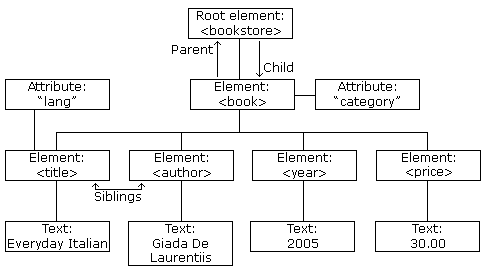
\includegraphics[width=\textwidth]{figures/nodetree}
\caption{Raamatupoe hierarhiline struktuur \citep{XML}}
\end{figure}

Joonise 1 kujutamine XML-kujul \citep{XML}:\\


\begin{lstlisting}
<?xml version="1.0" encoding="UTF-8"?>
<bookstore>
  <book category="cooking">
    <title lang="en">Everyday Italian</title>
    <author>Giada De Laurentiis</author>
    <year>2005</year>
    <price>30.00</price>
  </book>
  <book category="children">
    <title lang="en">Harry Potter</title>
    <author>J K. Rowling</author>
    <year>2005</year>
    <price>29.99</price>
  </book>
  <book category="web">
    <title lang="en">Learning XML</title>
    <author>Erik T. Ray</author>
    <year>2003</year>
    <price>39.95</price>
  </book>
</bookstore>
\end{lstlisting}

XML-i võib vaadata kui reeglite kogumikku, milles talletatakse informatsiooni semantiliste märgendite abil. Märgendid (\emph{tags}) on \emph{<>} märkide vahel olevad muutujad ja igal märgendil peab olema lõpumärgend (nt \emph{<bookstore>} ja \emph{</bookstore>}). XML dokument koosneb kolmest osast: proloog, dokumendi element ja epiloog. Faili alustatakse proloogiga, mis defineerib XML-i versiooni ja kasutatava kodeeringu. Dokumendi element on juurelement, mida saab olla vaid üks. Joonise 1 juurelement on \emph{<bookstore>}, mille alluvaks on elemendid \emph{<book>}. Märgenditel võib olla atribuut kui ka sisu, kuid need pole ilmtingimata kohustuslikud. Selles XML-koodijupis on raamatutel defineeritud ka atribuut \emph{category}, mille väärtus oleneb raamatu valdkonnast. Elemendi \emph{<book>} alluvateks on \emph{<title>}, \emph{<author>}, \emph{<year>} ja \emph{<price>}, mis on omakorda teineteise kolleegid. Kõigil neil elementidel on sisu ja elemendil \emph{<title>} on ka atribuut \emph{lang}, mille väärtuseks on keel. Viimane rida (\emph{</bookstore>}) ütleb, et see on juurelemendi lõpp ja ühtlasi ka dokumendi keha lõpp. See tähendab, et rohkem raamatuid selles raamatupoes ei eksisteeri. \citep{XML}

Märgendite abil pannakse paika andmete loogiline struktuur. XML-il pole eeldefineeritud märgendeid. Seega igal inimesel on võimalik defineerida oma vajadustele vastav struktuur ehk süntaks, mis paneb paika elemendi nimetused ja järjestuse. Oluline on, et kasutaja poolt defineeritud süntaks vastaks XML-i rangetele reeglitele:

\begin{enumerate}
    \item eksisteerib juurelement;
    \item elementidel peab olema lõpumärgend;
    \item elementide pesitsemine ehk üksteise sees paiknemine (\emph{nesting}) on rangelt määratletud;
    \item atribuutide väärtused peavad olema jutumärkides.
    \citep{XML}
\end{enumerate}

Kui kasutaja loob enda märgenduse, siis XML-protsessoril pole võimalik selle valiidsuses veenduda, sest pole midagi millegagi võrrelda. Selleks tuleb kasutajal XML-dokumendis defineerida kasutatav süntaks. XML-dokumentide valideerimiseks on kaks viisi: dokumenditüübi definitsioon (\emph{document type definition} -- DTD) ja XML-skeema (\emph{XML schema}). Nende asukoht on vahetult peale XML-versiooni deklaratsiooni ja kindlasti enne dokumendi keha. Juhul kui XML-dokument on DTD või XML skeemaga vastavuses, siis on ka XML-dokument kehtiv. \citep{XML}

\subsection{Sõnaliikide kitsaskohad}

``Kas tegelik tekst allub eesti keele morfoloogilistele kirjeldustele'' (Heiki-Jaan Kaalep, Kadri Muischnek, Kaili Müürisep, Andriela Rääbis, Külli Habicht).

Kadri Muischnek ja Kadri Vider ``Sõnaliigituse kitsaskohad eesti keele arvutianalüüsis''\\
Miskit saaks ka siit:\\
Rudolf Karelson ``Taas probleemidest sõnaliigi määramisel''\\
Tiit Hennoste artikkel ``Suulise kõne uurimine ja sõnaliigi probleemid'' või ``Suuline kõne ja morfoloogiaanalüsaator''\\ 

Üks huvitav artikkel Reili Arguselt on ``Imitatiivide kohast lastekeeles: reduplikatsioonist, morfoloogiast ja sõnaliigilisest ambivalentsusest'', kus räägitakse imitatiividest ja onomatopoeetilistest sõnadest. Ja see teema haakub väga palju praktilise osaga: morfanalüüsaatori kategooriad ei sobi hästi selliste sõnade jaoks.

AGA ma kindlasti ootan ettepanekuid!


\newpage
\section{CHILDES ja eesti keele alamkorpused}

Selles peatükis tutvustatakse CHILDES-i korpust ja eesti keele alamkorpuseid, mida siinkirjutaja kasutab tulevase magistritöö materjalina. Lisaks antakse lühiülevaade alamkorpuste standardiseerimise probleemidest.

\subsection{CHILDES}
CHILDES (\emph{Child Language Data Exchange System}) on \emph{Talkbank}i alamkorpus, mis loodi 1984. aastal Brian MacWhinney (Carnagie Melloni ülikool) ja Catherine Snow (Harvardi ülikool) poolt selleks, et koondada kokku erinevate keeleuurijate kogutud keelematerjali eesmärgiga, et need oleksid kõigile vabalt kättesaadavad ja võimaldaksid eri keelte uurijatel oma andmeid ja uurimistulemusi teiste keeltega võrrelda. CHILDES-ist on saanud mahukas, rahvusvaheline ja usaldusväärne andmebaas, mis sisaldab nii audio- ja videolindistusi kui ka standardsel viisil transkribeeritud tekste. \citep[1]{Gillis}

CHILDES-i süsteemi juures peab silmas pidama seda, et see funktsioneerib \emph{repositooriumina}. Repositooriumist võib mõelda kui laost või arhiivist, kuhu üles laetud materjali talletatakse digitaalselt. Repositooriumi jaoks on oluline, et korpused oleksid avalikult kättesaadavad ja standardsel viisil transkribeeritud ja et andmekogu oleks kooskõlas rahvusvaheliste standarditega. Seetõttu pakub CHILDES erinevaid tarkvaralisi töövahendeid, mida arendatakse ja kaasajastatakse kõigil platvormidel (\emph{Windows}, \emph{MacOS}, \emph{Unix}). \citep[1]{Gillis}

CHILDES-i andmebaas jaguneb nelja suurde kategooriasse:
\begin{enumerate}
    \item esimese keele omandamine;
    \item teise keele keele omandamine;
    \item kakskeelsus ja 
    \item kliinilised probleemid. \citep[1]{Gillis}
\end{enumerate}

Andmebaasi korpuste tekstide/lindistuste transkribeerimiseks/kodeerimiseks kasutatakse CHAT-käsiraamatut (\emph{Codes of the Human Analysis of Transcripts}, vt \citep{CHAT}). CHAT-käsiraamat on mõeldud selleks, et kõik lindistused/tekstid oleksid standardsel viisil transkribeeritud ja kodeeritud. Käsiraamatus on väga suur valik kodeeringuid, kuid transkribeerija ei ole kohustatud neid kõiki kasutama. Oluline oleks, et transkribeerimist ja kodeerimist tehakse vähemalt baastasemel. Lisaks CHAT-käsiraamatule on keeleuurijatel võimalus kasutada ka analüüsimistarkvara ja redaktorit CLAN (\emph{Computerized Language Analysis}), mis abistab keeleuurijat korpuse transkribeerimisel, kodeerimisel ja analüüsimisel. CLAN tarkvaraga loodud failiformaati nimetatakse CHAT-failiks ja see salvestatakse laiendiga .\emph{cha} (xxx.cha) \citep[1--2, 6]{Gillis} Talkbankis on kasutusel ka Chatter tarkvara, mis teostab CHAT-failide ranget valideerimist ja ka konverteerimist valiidseteks XML-failideks \citep{CHATTER}.

Hetkel on andmebaasis esindatud 39 keelt: germaani keeled (afrikaani, taani, hollandi, inglise, saksa, norra ja rootsi keel), romaani keeled (katalaani, prantsuse, itaalia, portugali, rumeenia ja hispaania keel), slaavi keeled (horvaadi, vene, serbia ja sloveenia keel), keldi keeled (iiri ja kõmri keel), afroaasia keeled (araabia, heebrea ja berberi keeled), hiina-tiibeti keeled (mandariini hiina, kantoniini, taiwani ja tai keel), draviidi keeled (tamili keel), uurali keeled (eesti ja ungari keel), indoiraani keeled (farsi keel), austroneesia keeled (indoneesia keel), kreeka, cree ja baski keeled. 2013. aasta maikuu seisuga koosnes andmebaas 13 miljonist lausungist ja rohkem kui 50 miljonist sõnavormist. Kõige suurema mahuga on esimesse kategooriasse kuuluvad ehk esimese keele korpused (11 miljonit lausungit ja 43 miljonit sõnavormi). Kõige enam on esindatud inglise, saksa ja prantsuse keel.\citep[2--5]{Gillis}

Transkriptsioonid algavad päisega (ingl k. \emph{header}), kus antakse informatsiooni lindistuse aja, koha, osalejate, kestuse, laste vanuse jms kohta. Põhiridadele paigutatakse kõnelejat tähistav kolmetäheline kood, millele järgneb  kõneleja tegelik kõne. Tegelikule kõnele lisatakse juurde, kas transkribeerija- või uurijapoolsed kommentaarid või kodeeringud (neid nimetatakse \emph{sõltridadeks}). Sõltridade arv oleneb keeleuurija eesmärkidest. Nagu suulise kõne puhulgi, pole ainuüksi verbaalse info järgi aru saada, millest hetkel jutt käib, seega tuleks transkribeerimisel kasutada vähemalt üht sõltrida, nt kommentaaririda. (\citealp[68]{Argus2007}; \citealp{CHAT}) Vt näide (1) ja (2).
\hfill

(1):
\begin{description}
    \item*MOT: arvuta need kõigepealt ära.
    \item*CHI: jah mm kaheksa miinus seitse on üks.
    \item*CHI: niimoodi kümme miinus üks on üheksa.
    \item\%com CHI kirjutab ja ise räägib samal ajal kaasa.
    \item(Kõrgesaar, gregory03.cha)
\end{description}
\hfill

(2)
\begin{description}
    \item*FAT:   köögis saab teritada , köögis on nuga .
    \item*MOT:   +< aga siin oli ka teritaja .
    \item*FAT:   jaa aga ma ei tea , kus see on .
    \item*CHI:   +< seda kätte .
    \item*FAT:   mida sa tahad kätte , issi ei tea , kus see teritaja on .
    \item*MOT:   see teritas väga ilusasti muidu .
    \item*CHI:   telita [*] .
    \item\%err:   terita=teritaja \$MOR
    \item\%par:   CHI aevastab
    \item(Vija, 20008.cha)
\end{description}


\subsection{Alamkorpuste standardiseerimise probleemid}

\emph{TO-DO}:\\
SIIN TAHAKS KIRJUTADA KA ``From CHILDES to TalkBank'' (Brian MacWhinney, CHILDES-i asutaja), sest siin tuuakse välja üldised transkriptsiooni probleemid.\\
SIIN tahaks puudutada ka morfoloogiliste vigade teemat (et mida veaks pidada, vea liigitusprobleemist, vigade transkribeerimis- ja kodeerimisprobleemidest, veakodeerimisvõimalustest ja see kõik puudutab CHILDES-it). Aluseks oleks Arguse artikkel ``Eesti lastekeelekorpuse morfoloogiliste vigade
märgendamisest ja liigitamisest''.\\
\emph{END-TO-DO}

Reili Argus kirjeldab oma artiklis \citep{Argus2007} mõningaid transkribeerimise ja CHILDES-i tarkvara kasutamisega seonduvaid probleeme.

Esiteks, CLAN-i analüüsitarkvara on mõeldud inglise keelele, seega tuleb eesti keele analüüsimisel arvestada sellega, et eesti keel on võrreldes inglise keelega sünteetilisema süsteemiga keel. Seega, kui keeleuurija tahab CLAN-i tarkvara kasutades teha mingisuguseid sagedusloendeid, siis ei saada adekvaatseid tulemusi. Näiteks lekseemi \emph{kala} kolm sõnavormi \emph{kala}, \emph{kalaga}, \emph{kalale} loetakse programmi poolt eri lekseemideks. Selline asjaolu põhjustab ka statistiliselt väärate arvude tekkimist. Homonüümide eristamist tuleb teha näiteks käsitsi.\citep[70]{Argus2007}

Argus väidab, et kuna lindistuste transkribeerimisel kasutatakse kuuldeortograafiat, siis need transkriptsioonid ei anna tõetruud pilti sellest, milline on lapse tegelik keelekasutus. Kui juba suulise kõne automaatne analüüsimine on keeruline, siis on lapse suulise keele analüüsimine veel keerukam. Lindistuste puhul on tegemist spontaanse suulise kõnega, mis sisaldab elemente, mida pole tarvis analüüsida, nt häälitsused. Seega selleks, et korpuseid oleks võimalik analüüsida nii, et need annaksid keelekasutuse kohta autentse pildi, ja et oleks võimalik neid standardsele kujule viia, tuleb alustada juba korpuse tekstide transkribeerimise tasandist. \citep[71]{Argus2007}

Teiseks, probleeme tekitab see, et lapse puhul on tegemist ju areneva keelekasutusega, milles esineb palju erilisi tunnuseid, nt sõnakordus. Näiteks, kui sellist lausungit transkribeeritakse nii \emph{*CHI: onu, onu, onu}, siis tähendab see seda, et lapse lausung koosneb kolmest sõnavormist, aga kui näiteks transkribeerida seda lausungit viisil \emph{*CHI: onu [/] onu [/] onu [/]}, siis koosneb see lausung ühest sõnavormist, kuna CLAN-süsteem kohtleb seda kui korduvat üksust. Lisaks sõnakordusele on probleemiks ka onomatopoeetilised sõnad, mida esineb lapsekeeles väga palju ja seetõttu tuleb transkribeerimisel läbi mõelda, kuidas selliseid juhtumeid lahendada. CHAT-käsiraamat soovitab onomatopoeetiliste sõnade lõppu lisada sümbol \emph{@} \citep[72--73]{Argus2007}, aga reaalsuses kasutatakse seda ikka väga vähe ja see omakorda põhjustab seda, et transkriptsioonid ei järgi ühtset märgendamisstiili.

Võrreldes täiskasvanutega esineb lapsekeeles rohkem vigaseid vorme. Transkribeerimisel (nt vigade korral) on oluline, et transkribeerija peab nägema ja teadma seda, mida tegelikult öelda taheti, ja vastavad kodeeringud ka transkriptsiooni lisama nii, et vead oleksid juba esimesel tasandil liigitatud. \citep[74]{Argus2007} Kahjuks praegused alamkorpused pole veakodeerimise osas järjepidevad, kord on viga kodeeritud ühtmoodi, kord teistmoodi ja vahel üldse mitte. Näites (2) on viga põhireal kodeeritud kooloniga (\emph{:}), mille järele lisatakse korrektne sõnavorm. Näites (3) on veakodeerimine hoopis teine: põhireal järgneb vigasele sõnale [*] ja sõltreale on lisatud vearida (\emph{\%err}), kus  toimub vea lahtikodeerimine ja sümboli \emph{=} järele lisatakse korrektne vorm. Näites (4) on viga üldse kodeerimata jäetud.\\
\hfill

(2)
\begin{description}
    \item*FAT: kriit pane tahvli peale .
    \item*CHI: kit [: kriit] .
    \item*CHI: kit [: kriit] (.) vahvlile [= tahvlile] pääle [: peale] .
    \item(Vija; 20007.cha)
\end{description}
\hfill

(3)
\begin{description}
    \item*CHI: issi , loe seda .
    \item*CHI: issi , nüüd see [*] ei pane kinni !
    \item\%err: see=seda \$MOR
    \item(Vija; 20007.cha)
\end{description}
\hfill

(4)
\begin{description}
    \item*FAT: viskad minema või?
    \item*FAT: kus sa viskad selle?
    \item*CHI: kinn.
    \item*FAT: sinna viskad jah.
    \item(Kõrgesaar; arabella01f.cha)
\end{description}
\hfill


Morfoloogiliselt märgendatud korpuse loomine on väga vajalik, sest CHILDES-i analüüsitarkvara ei võimalda eesti keele morfoloogilist analüüsimist ja selle käsitsi tegemine oleks väga ajamahukas töö. Seega, praegusel hetkel on lapsekeele uurijatel automaatse statistika tegemine raskendatud ja paraku tehakse distributsioonianalüüse käsitsi \citep[78]{Argus2007}.

\subsection{Eesti keele alamkorpuste struktuur}

CHILDES-i andmebaasis on eesti laste suulise kõne lindistused olnud alates 1998. aastast. 2016. aasta märtsikuu seisuga koosneb eesti lastekeele korpus seitsmest alamkorpusest, mis on oma nimed saanud korpuse koostajate järgi: Argus, Beek, Kapanen, Kohler, Kõrgesaar, Vija ja Zupping \citep{CHILDES}. Tabelid 1--7 kajastavad laste vanuselist jaotumist alamkorpuste lõikes. Lisaks on välja toodud ka lapse nimi ja sugu, lapsega tehtud sessioonide arv, lapse ja lapsele suunatud kõne ehk hoidjakeele sõnade arv igas sessioonis. \emph{Sõna} all mõeldakse tekstisõna ehk tühikute vahele jäävat tähtede järjendit. Töös on kasutusel ka termin \emph{sõnavorm}, mis tähistab leksikaalse sõna üht grammatilist vormi ja moodustab sõnavara ehk leksikoni.

\hfill

\begin{table}[H]
\centering
\caption{Vija korpus}
\resizebox{\textwidth}{!}{
\begin{tabular}{|l|l|c|c|c|c|c|}
\hline
Lapse nimi               & Vanus    & \multicolumn{1}{l|}{Sugu} & \multicolumn{1}{l|}{Sessioonid} & \multicolumn{1}{l|}{Lapse sõnad} & \multicolumn{1}{l|}{Hoidja sõnad} & \multicolumn{1}{l|}{KOKKU} \\ \hline\hline
\multirow{3}{*}{Andreas} & 1;7-1;11 & \multirow{3}{*}{p}        & 7                               & 2845                             & 8521                              & 11366                      \\ \cline{2-2} \cline{4-7} 
                         & 2;0-2;8  &                           & 37                              & 41498                            & 59272                             & 100770                     \\ \cline{2-2} \cline{4-7} 
                         & 3;0-3;1  &                           & 30                              & 66038                            & 48137                             & 114175                     \\ \hline\hline
KOKKU                    & \multicolumn{2}{l|}{}                & 74                              & 110381                           & 115930                            & 226311                     \\ \hline
\end{tabular}}
\end{table}
\hfill

\begin{table}[H]
\centering
\caption{Arguse korpus}
\resizebox{\textwidth}{!}{
\begin{tabular}{|l|l|c|c|c|c|c|}
\hline
Lapse nimi               & Vanus    & \multicolumn{1}{l|}{Sugu} & \multicolumn{1}{l|}{Sessioonid} & \multicolumn{1}{l|}{Lapse sõnad} & \multicolumn{1}{l|}{Hoidja sõnad} & \multicolumn{1}{l|}{KOKKU} \\ \hline\hline
\multirow{2}{*}{Hendrik} & 1;8-1;11 & \multirow{2}{*}{p}        & 5                               & 566                              & 1963                              & 2529                       \\ \cline{2-2} \cline{4-7} 
                         & 2;0-2;5  &                           & 12                              & 3654                             & 7190                              & 10844                      \\ \hline\hline
KOKKU                    & \multicolumn{2}{l|}{}                & 17                              & 4220                             & 9153                              & 13373                      \\ \hline
\end{tabular}}
\end{table}
\hfill


\begin{table}[H]
\centering
\caption{Kõrgesaare korpus}
\resizebox{\textwidth}{!}{
\begin{tabular}{|l|l|c|c|c|c|c|}
\hline
Lapse nimi               & Vanus      & \multicolumn{1}{l|}{Sugu} & \multicolumn{1}{l|}{Sessioonid} & \multicolumn{1}{l|}{Lapse sõnad} & \multicolumn{1}{l|}{Hoidja sõnad} & \multicolumn{1}{l|}{KOKKU} \\ \hline\hline
Andri                    & 11;7-11;9  & p                         & 2                               & 4253                             & 4445                              & 8698                       \\ \hline
Arabella                 & 11;8       & t                         & 1                               & 200                              & 2439                              & 2639                       \\ \hline
Artur                    & 1;4        & p                         & 1                               & 94                               & 3540                              & 3634                       \\ \hline
\multirow{5}{*}{Gregory} & 6;6        & \multirow{5}{*}{p}        & 1                               & 3435                             & 4570                              & 8005                       \\ \cline{2-2} \cline{4-7} 
                         & 7;1-7;8    &                           & 2                               & 4501                             & 7559                              & 12060                      \\ \cline{2-2} \cline{4-7} 
                         & 8;4-8;10   &                           & 3                               & 4840                             & 5823                              & 10663                      \\ \cline{2-2} \cline{4-7} 
                         & 9;7-9;8    &                           & 2                               & 3927                             & 4125                              & 8052                       \\ \cline{2-2} \cline{4-7} 
                         & 10;5       &                           & 2                               & 4822                             & 4740                              & 9562                       \\ \hline
\multirow{8}{*}{Harley}  & 4;0-4;1    & \multirow{7}{*}{p}        & 5                               & 1357                             & 3269                              & 4626                       \\ \cline{2-2} \cline{4-7} 
                         & 7;2        &                           & 3                               & 3589                             & 3208                              & 6797                       \\ \cline{2-2} \cline{4-7} 
                         & 10;1-10;2  &                           & 2                               & 3232                             & 3355                              & 6587                       \\ \cline{2-2} \cline{4-7} 
                         & 11;0-11;11 &                           & 4                               & 7838                             & 6716                              & 14554                      \\ \cline{2-2} \cline{4-7} 
                         & 12;5       &                           & 1                               & 2003                             & 1344                              & 3347                       \\ \cline{2-2} \cline{4-7} 
                         & 13;2-13;3  &                           & 2                               & 4290                             & 4261                              & 8551                       \\ \cline{2-2} \cline{4-7} 
                         & 14;0-14;1  &                           & 2                               & 4976                             & 4665                              & 9641                       \\ \cline{2-7} 
                         & 4;0        & t                         & 2                               & 412                              & 870                               & 1282                       \\ \hline
Hellyn                   & 8;7        & t                         & 1                               & 1438                             & 2066                              & 3504                       \\ \hline
Jaana                    & 2;5        & t                         & 1                               & 1447                             & 1841                              & 3288                       \\ \hline
Kaisa                    & 5;8-5;9    & t                         & 2                               & 3256                             & 4690                              & 7946                       \\ \hline
Mia                      & 2;3        & t                         & 1                               & 1643                             & 5368                              & 7011                       \\ \hline
Olivia                   & 3;2        & t                         & 1                               & 1275                             & 2882                              & 4157                       \\ \hline
\multirow{3}{*}{Ruuben}  & 1;3-1;4    & \multirow{3}{*}{p}        & 2                               & 777                              & 3544                              & 4321                       \\ \cline{2-2} \cline{4-7} 
                         & 2;2        &                           & 1                               & 936                              & 3355                              & 4291                       \\ \cline{2-2} \cline{4-7} 
                         & 3;6        &                           & 1                               & 1259                             & 2669                              & 3928                       \\ \hline
Sirlin                   & 1;3        & t                         & 1                               & 19                               & 2348                              & 2367                       \\ \hline\hline
KOKKU                    & \multicolumn{2}{l|}{}                  & 46                              & 65819                            & 93692                             & 159511                     \\ \hline
\end{tabular}}
\end{table}
\hfill

\begin{table}[H]
\centering
\caption{Beeki korpus}
\resizebox{\textwidth}{!}{
\begin{tabular}{|l|l|c|c|c|c|c|}
\hline
Lapse nimi               & Vanus    & \multicolumn{1}{l|}{Sugu} & \multicolumn{1}{l|}{Sessioonid} & \multicolumn{1}{l|}{Lapse sõnad} & \multicolumn{1}{l|}{Hoidja sõnad} & \multicolumn{1}{l|}{KOKKU} \\ \hline\hline
\multirow{3}{*}{Liisbet} & 0;9-0;11 & \multirow{3}{*}{t}        & 6                               & 1450                             & 11487                             & 12937                      \\ \cline{2-2} \cline{4-7} 
                         & 1;0-1;2  &                           & 5                               & 1143                             & 10463                             & 11606                      \\ \cline{2-2} \cline{4-7} 
                         & 2;0-2;5  &                           & 9                               & 7571                             & 27022                             & 34593                      \\ \hline\hline
KOKKU                    & \multicolumn{2}{l|}{}                & 20                              & 10164                            & 48972                             & 59136                      \\ \hline
\end{tabular}}
\end{table}


\begin{table}[H]
\centering
\caption{Kapaneni korpus}
\resizebox{\textwidth}{!}{
\begin{tabular}{|l|l|c|c|c|c|c|}
\hline
Lapse nimi               & Vanus    & \multicolumn{1}{l|}{Sugu} & \multicolumn{1}{l|}{Sessioonid} & \multicolumn{1}{l|}{Lapse sõnad} & \multicolumn{1}{l|}{Hoidja sõnad} & \multicolumn{1}{l|}{KOKKU} \\ \hline\hline
\multirow{3}{*}{Martina} & 1;3-1;11 & \multirow{3}{*}{t}        & 6                               & 7302                             & 17791                             & 25093                      \\ \cline{2-2} \cline{4-7} 
                         & 2;1-2;7  &                           & 4                               & 6831                             & 9831                              & 16662                      \\ \cline{2-2} \cline{4-7} 
                         & 3;1      &                           & 1                               & 1805                             & 2115                              & 3920                       \\ \hline\hline
KOKKU                    & \multicolumn{2}{l|}{}                & 11                              & 15938                            & 29737                             & 45675                      \\ \hline
\end{tabular}}
\end{table}


\begin{table}[H]
\centering
\caption{Zuppingu korpus}
\resizebox{\textwidth}{!}{
\begin{tabular}{|l|l|c|c|c|c|c|}
\hline
Lapse nimi             & Vanus    & \multicolumn{1}{l|}{Sugu} & \multicolumn{1}{l|}{Sessioonid} & \multicolumn{1}{l|}{Lapse sõnad} & \multicolumn{1}{l|}{Hoidja sõnad} & \multicolumn{1}{l|}{KOKKU} \\ \hline\hline
\multirow{4}{*}{Linda} & 1;3-1;11 & \multirow{4}{*}{t}        & 9                               & 3677                             & 15191                             & 18868                      \\ \cline{2-2} \cline{4-7} 
                       & 2;0-2;11 &                           & 12                              & 6785                             & 13114                             & 19899                      \\ \cline{2-2} \cline{4-7} 
                       & 3;0      &                           & 1                               & 542                              & 1052                              & 1594                       \\ \cline{2-2} \cline{4-7} 
                       & 4;2      &                           & 1                               & 628                              & 1472                              & 2100                       \\ \hline\hline
KOKKU                  & \multicolumn{2}{l|}{}                & 23                              & 11632                            & 30829                             & 42461                      \\ \hline
\end{tabular}}
\end{table}
\hfill

\begin{table}[H]
\centering
\caption{Kohleri korpus}
\resizebox{\textwidth}{!}{
\begin{tabular}{|l|l|c|c|c|c|c|}
\hline
Lapse nimi              & Vanus     & \multicolumn{1}{l|}{Sugu} & \multicolumn{1}{l|}{Sessioonid} & \multicolumn{1}{l|}{Lapse sõnad} & \multicolumn{1}{l|}{Hoidja sõnad} & \multicolumn{1}{l|}{KOKKU} \\ \hline\hline
\multirow{2}{*}{Anna}   & 1;10-1;11 & \multirow{2}{*}{t}        & 4                               & 550                              & 4298                              & 4848                       \\ \cline{2-2} \cline{4-7} 
                        & 2;0-2;1   &                           & 3                               & 645                              & 3454                              & 4099                       \\ \hline
Carlos                  & 1;7-1;10  & p                         & 9                               & 1797                             & 6809                              & 8606                       \\ \hline
Helen                   & 1;1-1;10  & t                         & 7                               & 551                              & 7745                              & 8296                       \\ \hline
Henri                   & 2;2-2;3   & p                         & 3                               & 633                              & 2612                              & 3245                       \\ \hline
Mari                    & 2;5-2;8   & t                         & 7                               & 2455                             & 7850                              & 10305                      \\ \hline
\multirow{2}{*}{Sandor} & 1;2-1;10  & p                         & 7                               & 1219                             & 9445                              & 10664                      \\ \cline{2-7} 
                        & 2;2       & p                         & 3                               & 1374                             & 4564                              & 5938                       \\ \hline
\multirow{2}{*}{Stella} & 0;11      & \multirow{2}{*}{t}        & 1                               & 6                                & 295                               & 301                        \\ \cline{2-2} \cline{4-7} 
                        & 1;0-1;6   &                           & 8                               & 287                              & 6629                              & 6916                       \\ \hline
Taimo                   & 1;5-1;11  & p                         & 9                               & 536                              & 6958                              & 7494                       \\ \hline\hline
KOKKU                   & \multicolumn{2}{l|}{}                 & 61                              & 10053                            & 60659                             & 70712                      \\ \hline
\end{tabular}}
\end{table}

\begin{table}[H]
\centering
\caption{Alamkorpuste \% kogu korpuses}
\begin{tabular}{|l|c|c|}
\hline
Korpus    & \multicolumn{1}{l|}{Sõnade arv} & \multicolumn{1}{l|}{\% kogu korpuses} \\ \hline\hline
Vija      & 226311                          & 37\%                                  \\ \hline
Kõrgesaar & 159511                          & 26\%                                  \\ \hline
Argus     & 13373                           & 2\%                                   \\ \hline
Beek      & 59136                           & 10\%                                  \\ \hline
Kapanen   & 45675                           & 7\%                                   \\ \hline
Zupping   & 42461                           & 7\%                                   \\ \hline
Kohler    & 70712                           & 11\%                                  \\ \hline
KOKKU     & 617179                          & 100\%                                 \\ \hline\hline
\end{tabular}
\end{table}

Kõige mahukamad on Vija, Kõrgesaare ja Kohleri korpused. Neist mahukaim on Vija korpus, moodustades kogu korpusest 37\%. Korpus sisaldab 226311 sõna, millest 110381 olid lapse sõnad ja 115930 hoidjasõnad. Lindistusi tehti Andreasega vahemikus 1;7--3;1 eluaastat. Kõrgesaare korpus moodustab kogu korpusest 26\% ja koosneb 159511 sõnast, neist 65819 on lapse sõnad ja 93692 hoidjasõnad. Materjal pärineb lindistustest 12 erineva lapsega vahemikus 1;3--14;1 eluaastat. Siia pole sisse arvestatud transkriptsioone vestlustest, mille osalejateks olid vaid täiskasvanud. Kohleri korpus moodustab kogu korpusest 11\% ja sisaldab 70712 sõna, lapse sõnade hulk 10053 ja hoidjakeele sõnade hulk 60659. Lindistusi tehti 8 erineva lapsega vahemikus 0;11--2;3 eluaastat.

Beeki korpus moodustab kogu korpusest 10\% ja sisaldab 59136 sõna, millest lapse sõnad on 10164 ja hoidjasõnad 48972. Lindistusi tehti Liisbetiga vahemikus 0;9--2;5 eluaastat. Kapaneni korpus moodustab kogu korpusest 7\%, sisaldades 45675 sõna, neist 15938 lapse sõnad ja 29737 hoidjakeele sõnad. Kapaneni materjal pärineb lindistustest Martinaga vahemikus 1;3--2;7 eluaastat. Zuppingu korpus moodustab samuti kogu korpusest 7\%, sisaldades 42461 sõna, neist 11632 on lapse sõnad ja 30829 hoidjakeele sõnad. Kõik lindistused on tehtud Lindaga vahemikus 1;3--4;2 eluaastat. Mahult kõige väiksem on Arguse korpus (2\%). Korpus sisaldab 13373 sõna, millest 4220 on lapse ja 9153 hoidjasõnad. Lindistusi tehti Hendrikuga vahemikus 1;8--2;5 eluaastat. CHILDES-i eesti keele alamkorpuse kogu suuruseks on 617179 sõna.


\subsubsection{Kõrgesaar}

Joonisel 2 on kujutatud lapse ja hoidja sõnade vanuselist jaotumist. Varasemalt olen kõiki vanuseid eristanud, kuid sellel joonisel on 10- ja 11-aastased ning 12-, 13- ja 14-aastased lapsed kokku pandud. Enamjaolt on kõigis vanusegruppides hoidja keele sõnad ülekaalus, v.a. 10--11- ja 12--14-aastased. 5-aastaste grupist alates on hoidja ja lapse sõnade osakaal mõnevõrra ``võrdsemalt'' jaotunud kui väiksemate lastega. 1-aastaste seas on hoidja sõnade osakaal lausa 92\% 
ja lapse sõnad vaid 8\%. 2-aastaste seas on hoidja sõnade osakaal 72\% ja lapse sõnad 28\%. 3- ja 4-aastaste laste puhul jaotuvad hoidja ja lapse sõnad enam-vähem ühesuguselt (69\% ja 31\% vs 70\% ja 30\%). 10--11-aastaste seas on lapse sõnade osakaal 51\% ja hoidja sõnu 49\%. 12--14-aastaste laste puhul on lapse sõnade osakaal 52\% ja hoidja sõnad 48\%.

\begin{figure}[H]
    \centering
    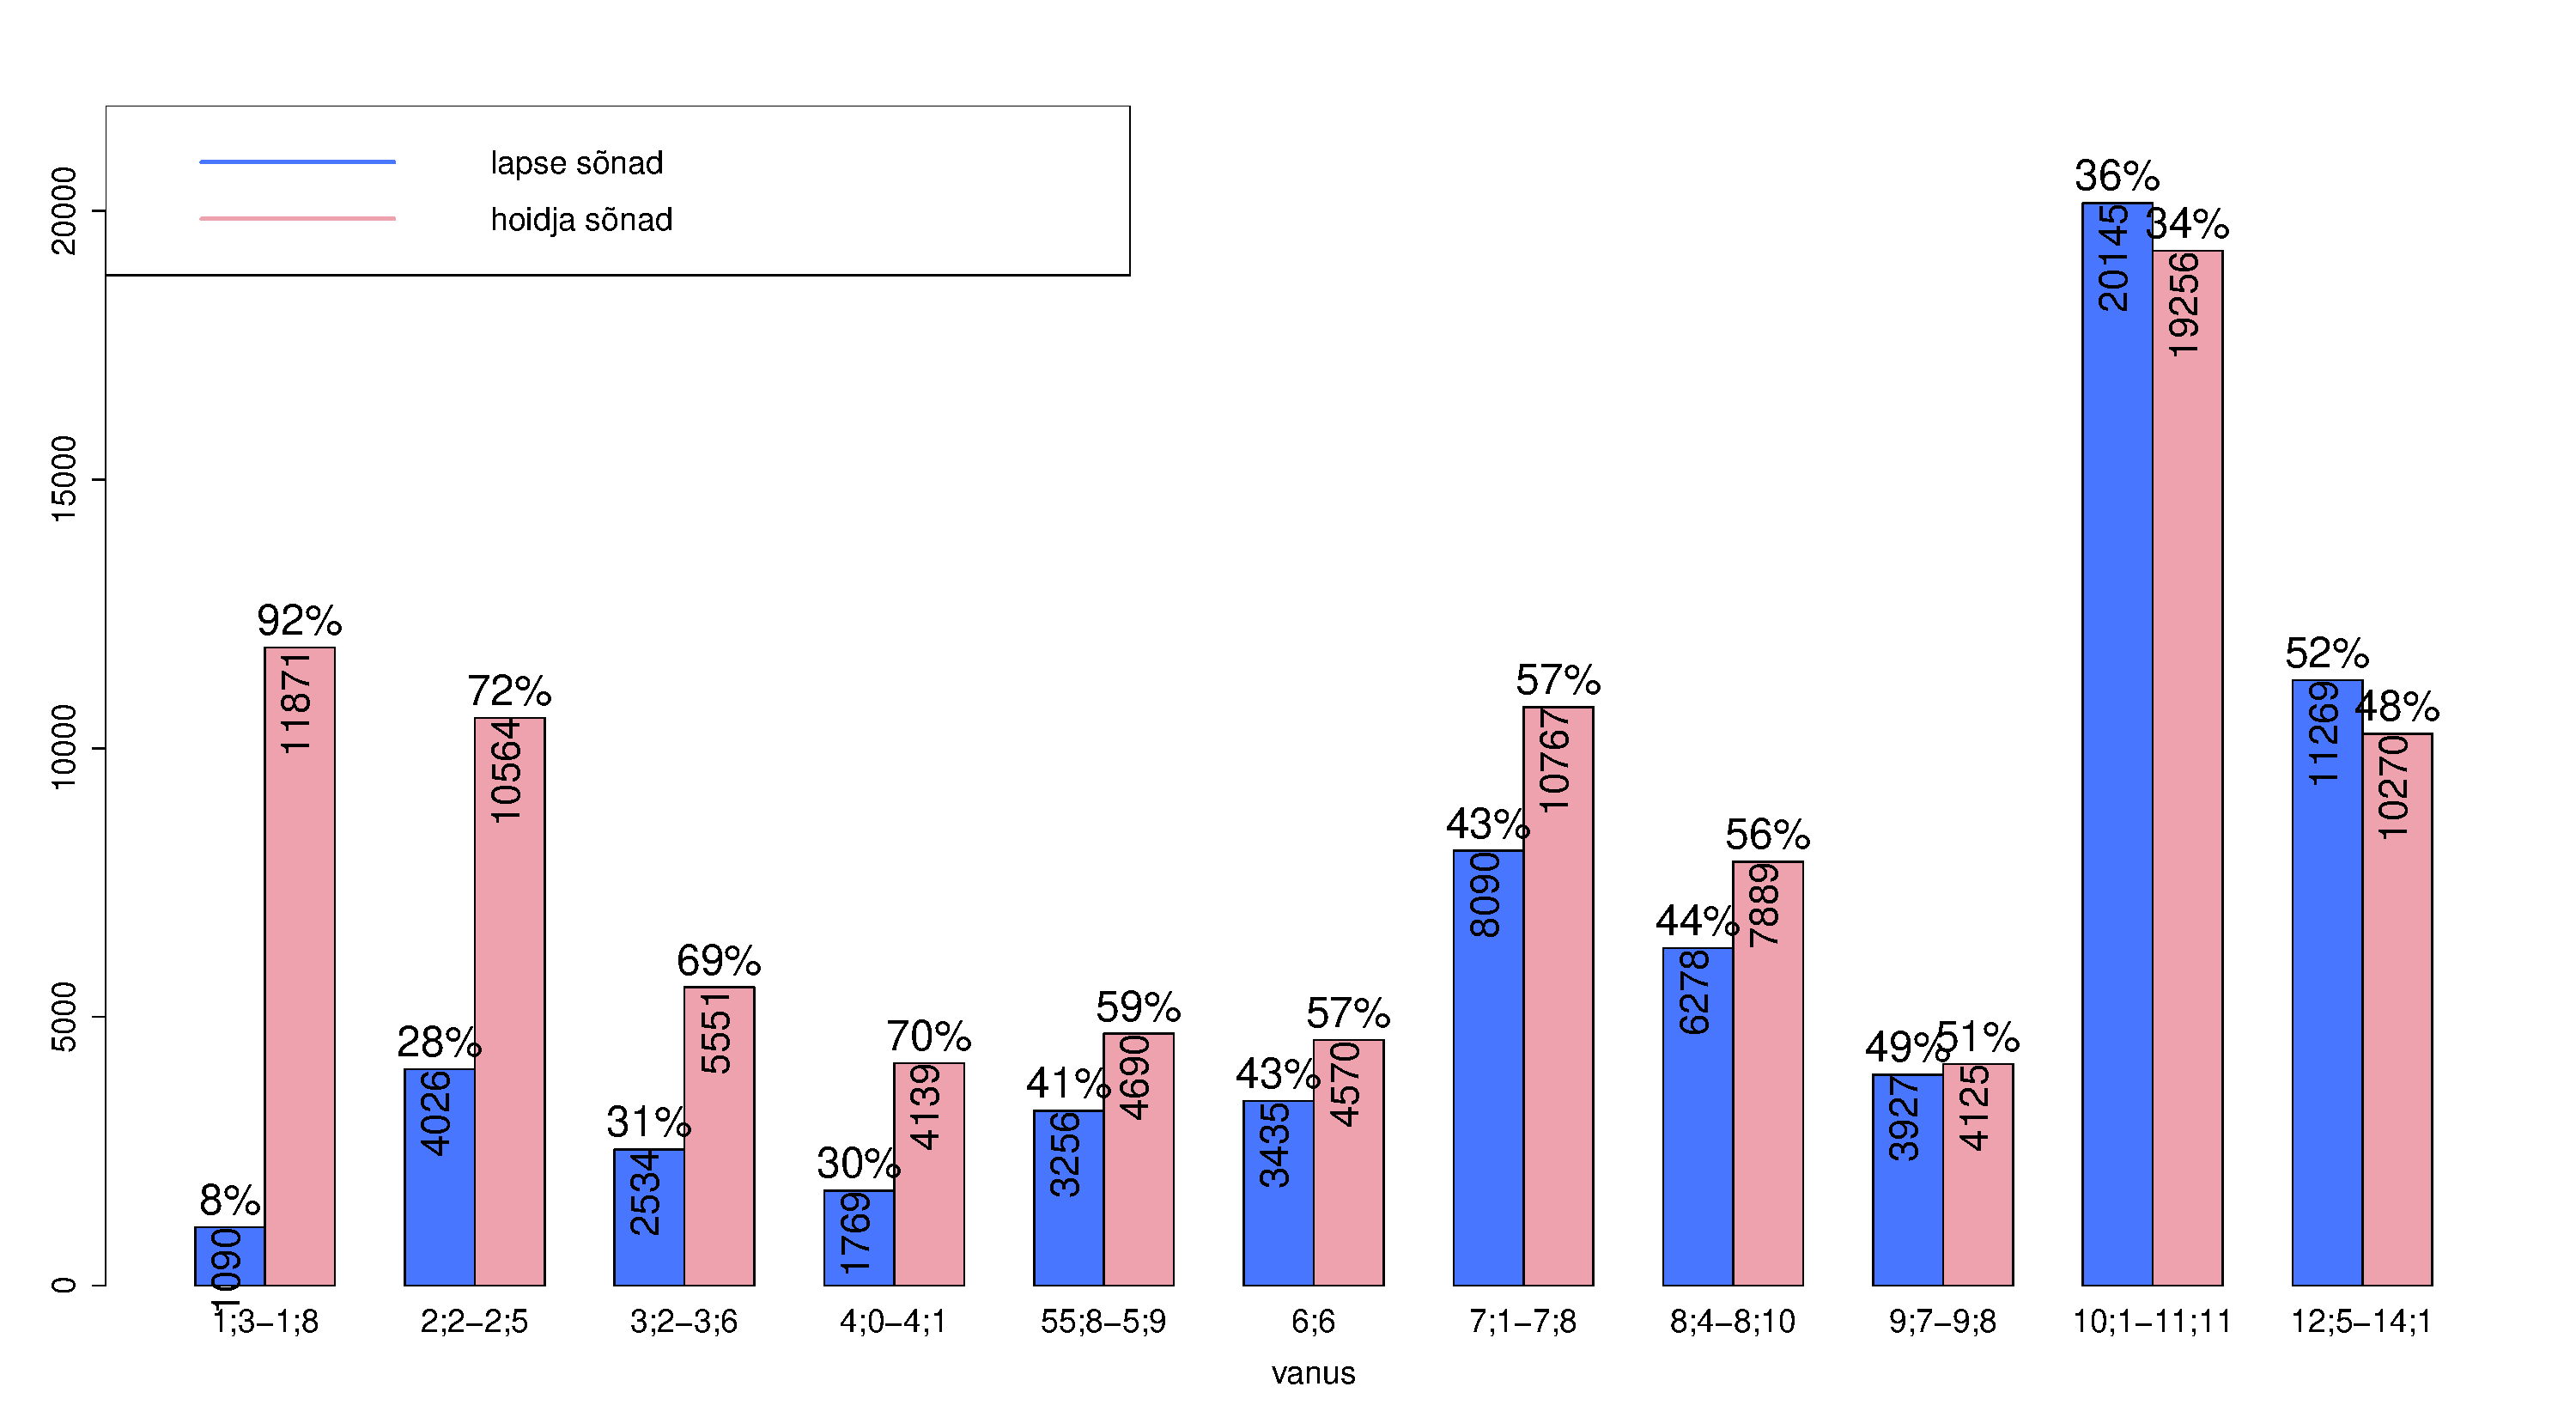
\includegraphics[width=\textwidth]{korgesaar_vanus_sonad}
    \caption{Kõrgesaar: lapse ja hoidja sõnade vanuseline jaotumine}
\end{figure}

Joonis 3 kujutab lapse ja hoidja sõnade soolist jaotumist. Nii tüdrukute kui ka poiste seas on ülekaalus hoidja sõnad, kuid poiste puhul on see jaotumine ühtlasem (56\% vs 70\%). Siinkohal peab arvesse võtma seda, et poistega tehtud sessioone oli rohkem kui tüdrukutega (37 sessiooni vs 9 sessiooni). Järelikult: mida rohkem sessioone, seda rohkem nii hoidja kui lapse sõnu. Vanuse kasvades hakkab laps loomult rohkem rääkima ja nii suureneb ka tema sõnade arv. Sellega saab põhjendada lapse ja hoidja sõnade võrdsemat jaotumist poiste seas, kuna Kõrgesaare korpuses on sessioonid vanuses 6--14 tehtud valdavalt poistega (8--aastaste ja 11-aastaste seas vaid üks sessioon tüdrukuga, vt tabel 3).

\begin{figure}[H]
    \centering
    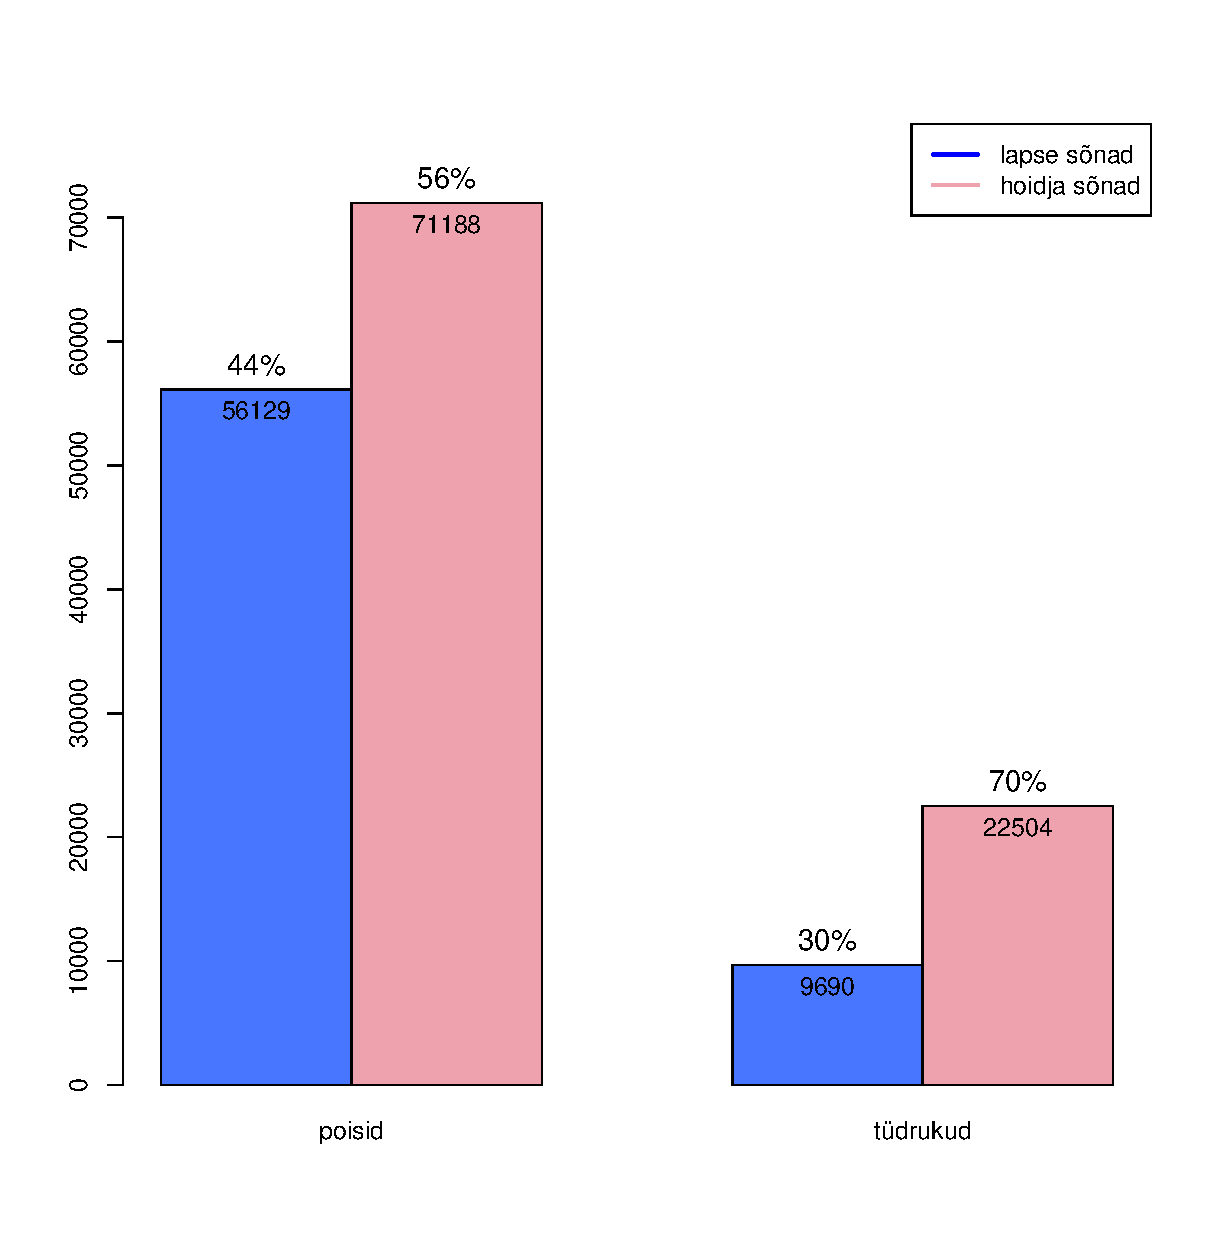
\includegraphics[width=11cm, height=12cm]{korgesaar_sugu_sonad}
    \caption{Kõrgesaar: lapse ja hoidja sõnade sooline jaotumine}
\end{figure}



\begin{figure}[H]
    \centering
    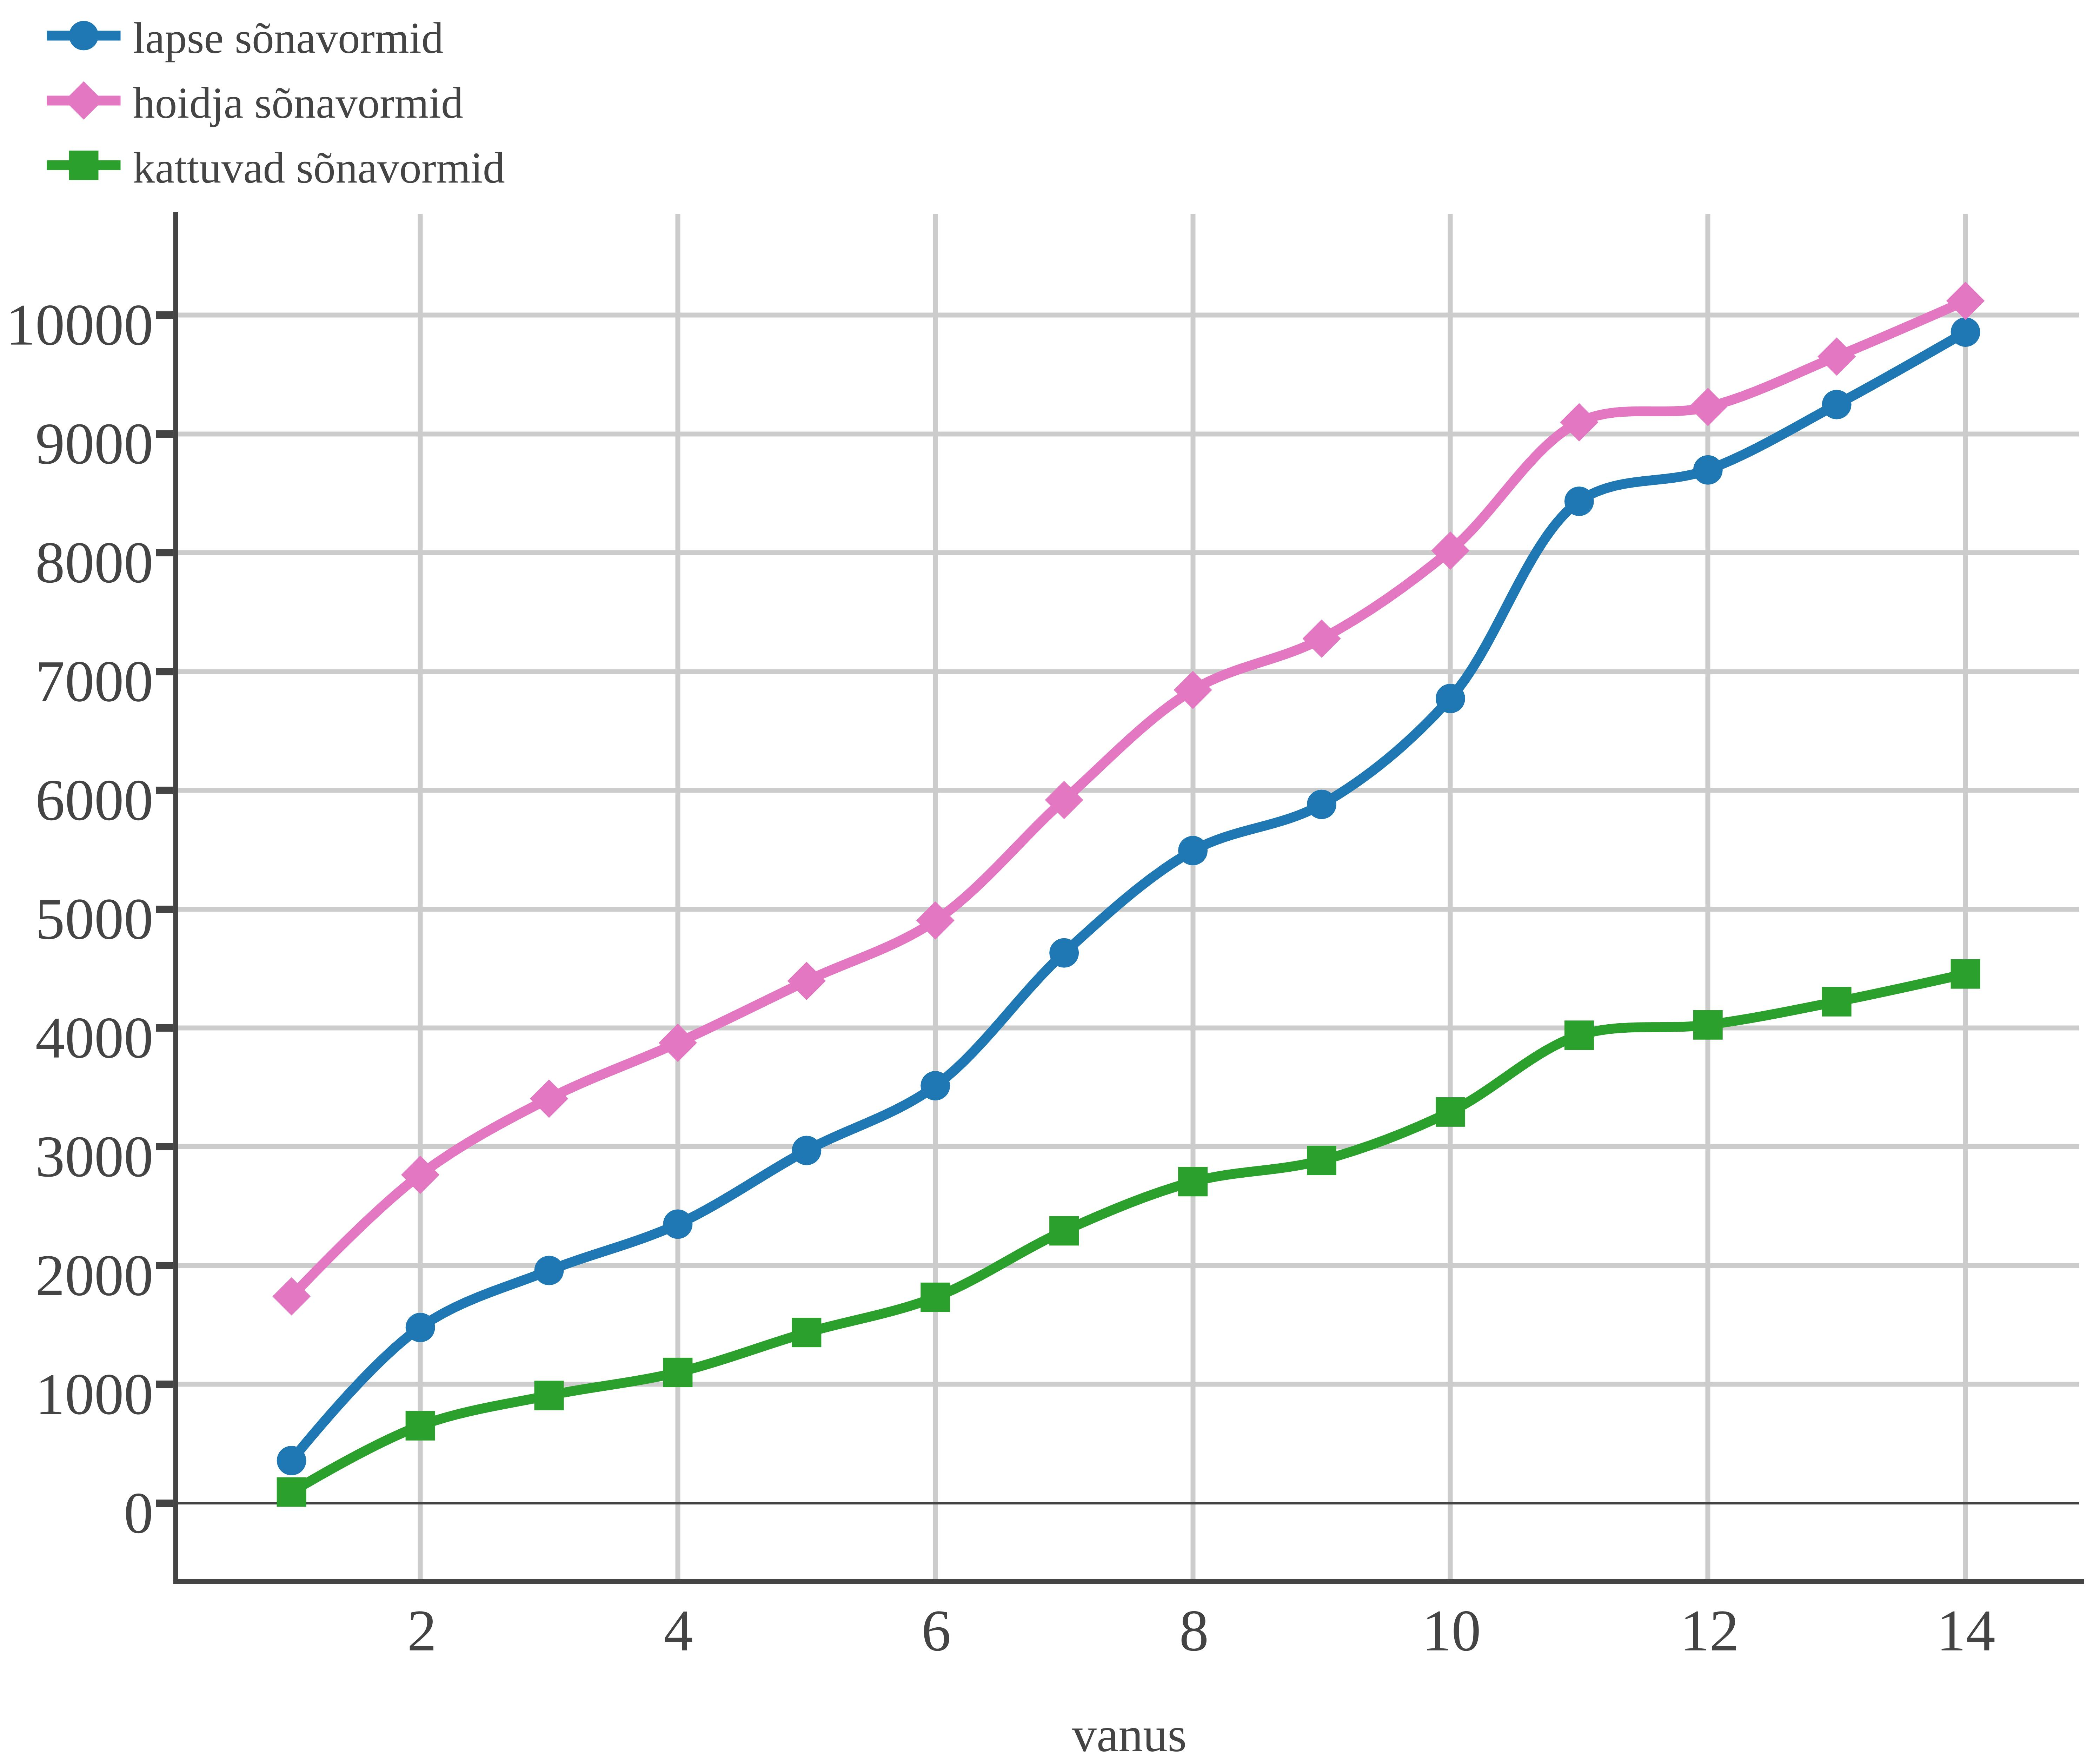
\includegraphics[width=11cm, height=9cm]{korgesaar_kum_crop}
    \caption{Kõrgesaar: sõnavormide kasv vanuseliselt}
\end{figure}

\begin{figure}[H]
    \centering
    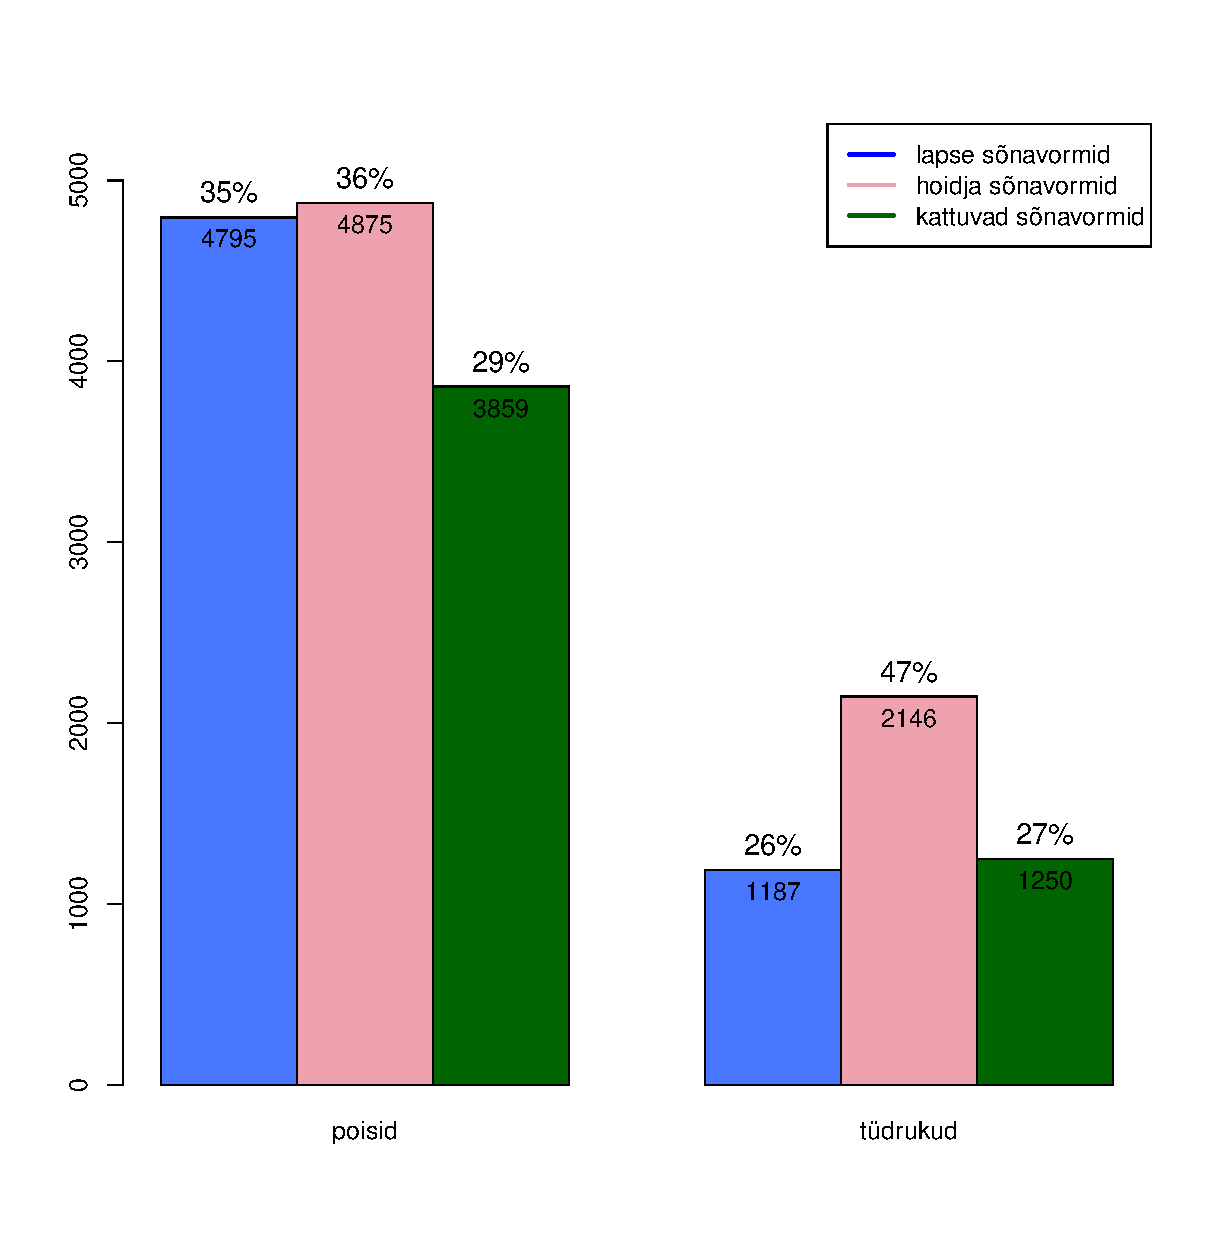
\includegraphics[width=11cm, height=9cm]{korgesaar_sugu}
    \caption{Kõrgesaar: sõnavormide sooline jaotumine}
\end{figure}




\subsubsection{Kapanen}

Joonisel 6 on kujutatud lapse ja hoidja sõnade vanuselist jaotumist. Kõigis vanusegruppides on hoidja keele sõnad ülekaalus. 2- ja 3-aastaste vanusegrupis on hoidja ja lapse sõnade osakaal mõnevõrra ``võrdsemalt'' jaotunud kui 1-aastaste laste seas. 2-aastaste seas on hoidja sõnu 59\% ja lapse sõnu 41\%. 3-aastaste seas on hoidja sõnu 54\% ja lapse sõnu 46\%. 1-aastaste seas on hoidja sõnu 71\% ja lapse sõnu 29\%.

\begin{figure}[H]
    \centering
    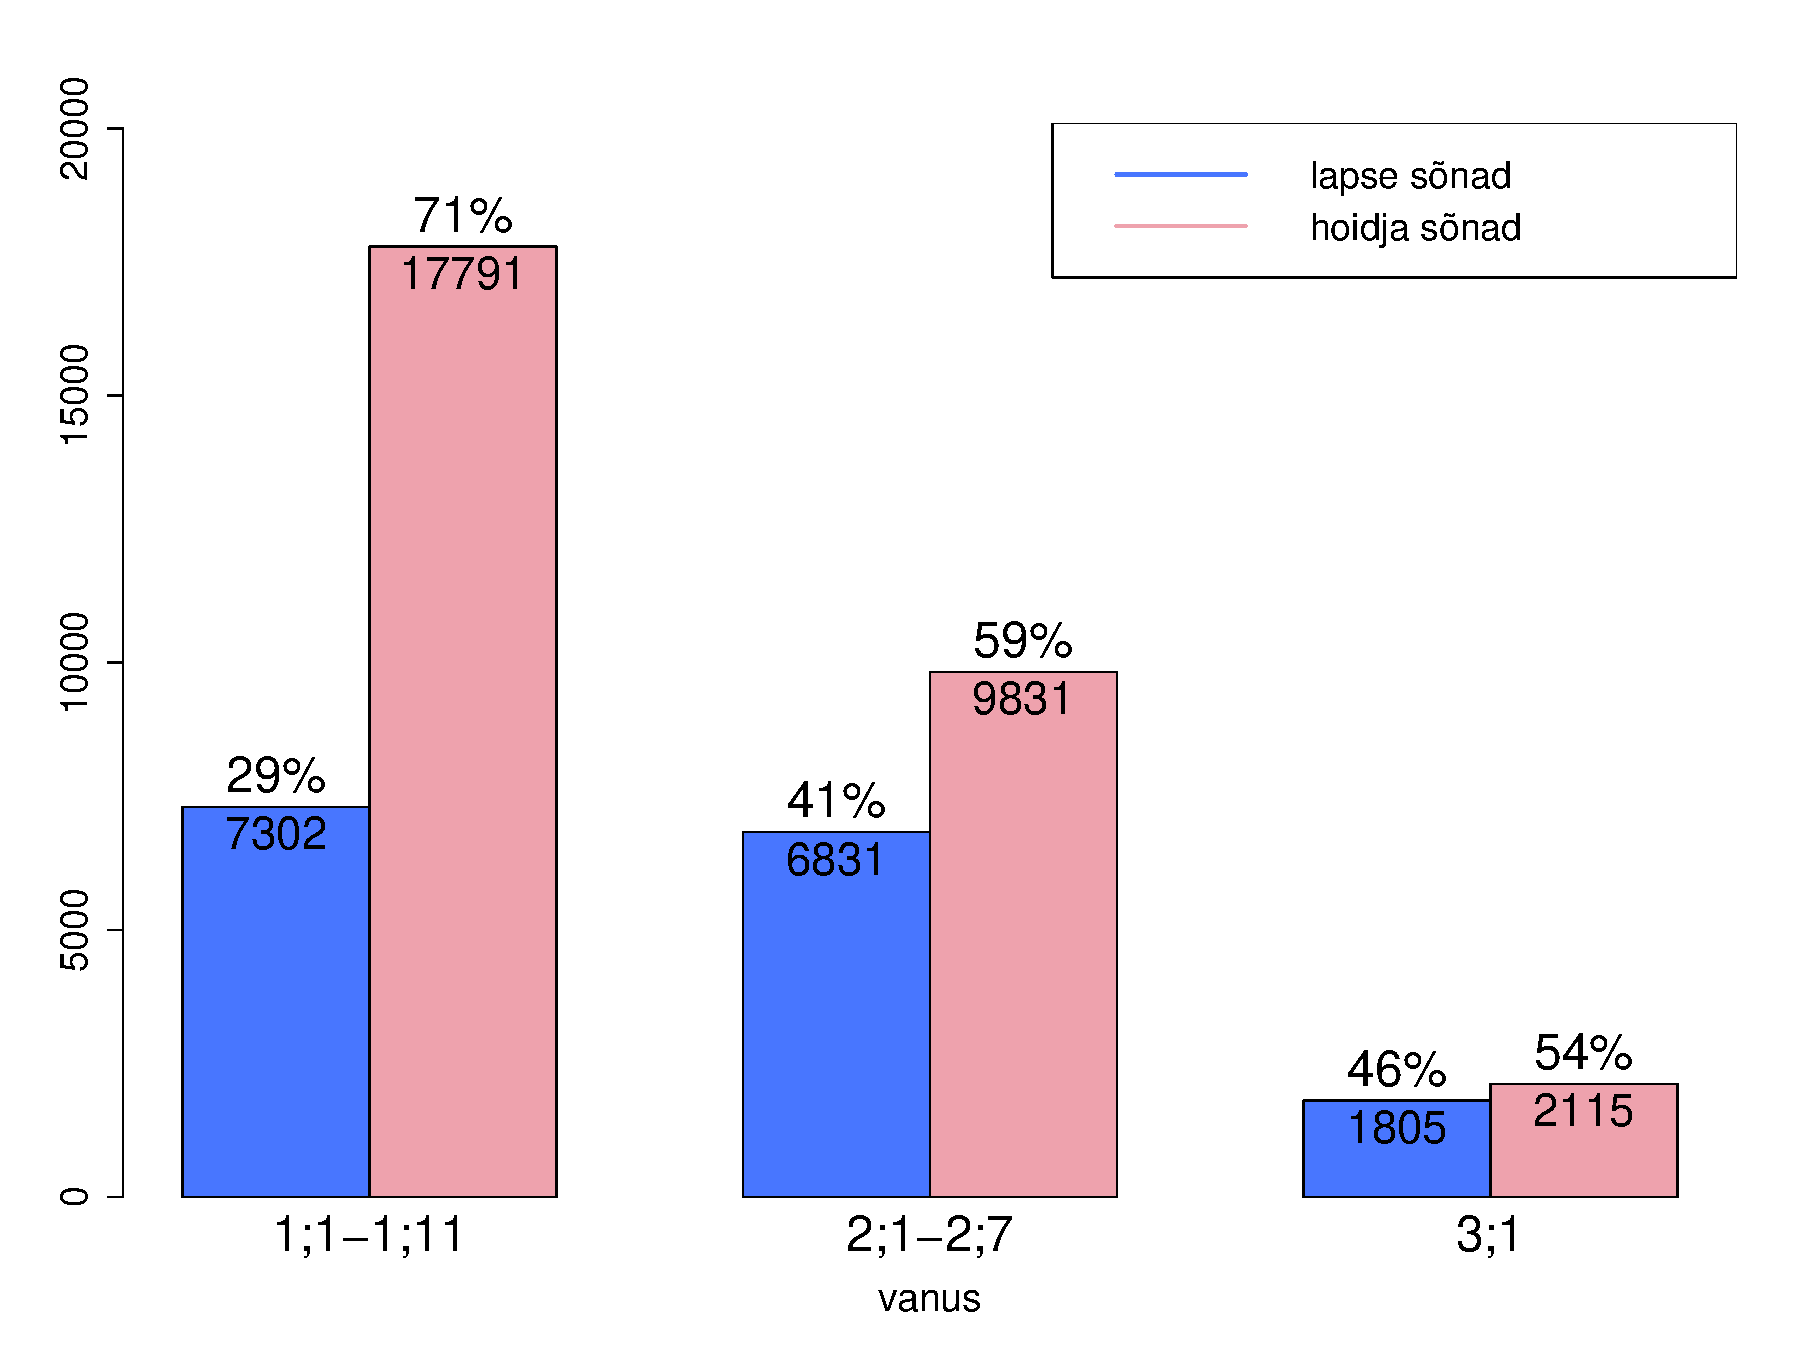
\includegraphics[width=\textwidth]{kapanen_vanus_sonad}
    \caption{Kapanen: lapse ja hoidja sõnade vanuseline jaotumine}
\end{figure}

% \begin{figure}[H]
%     \centering
%     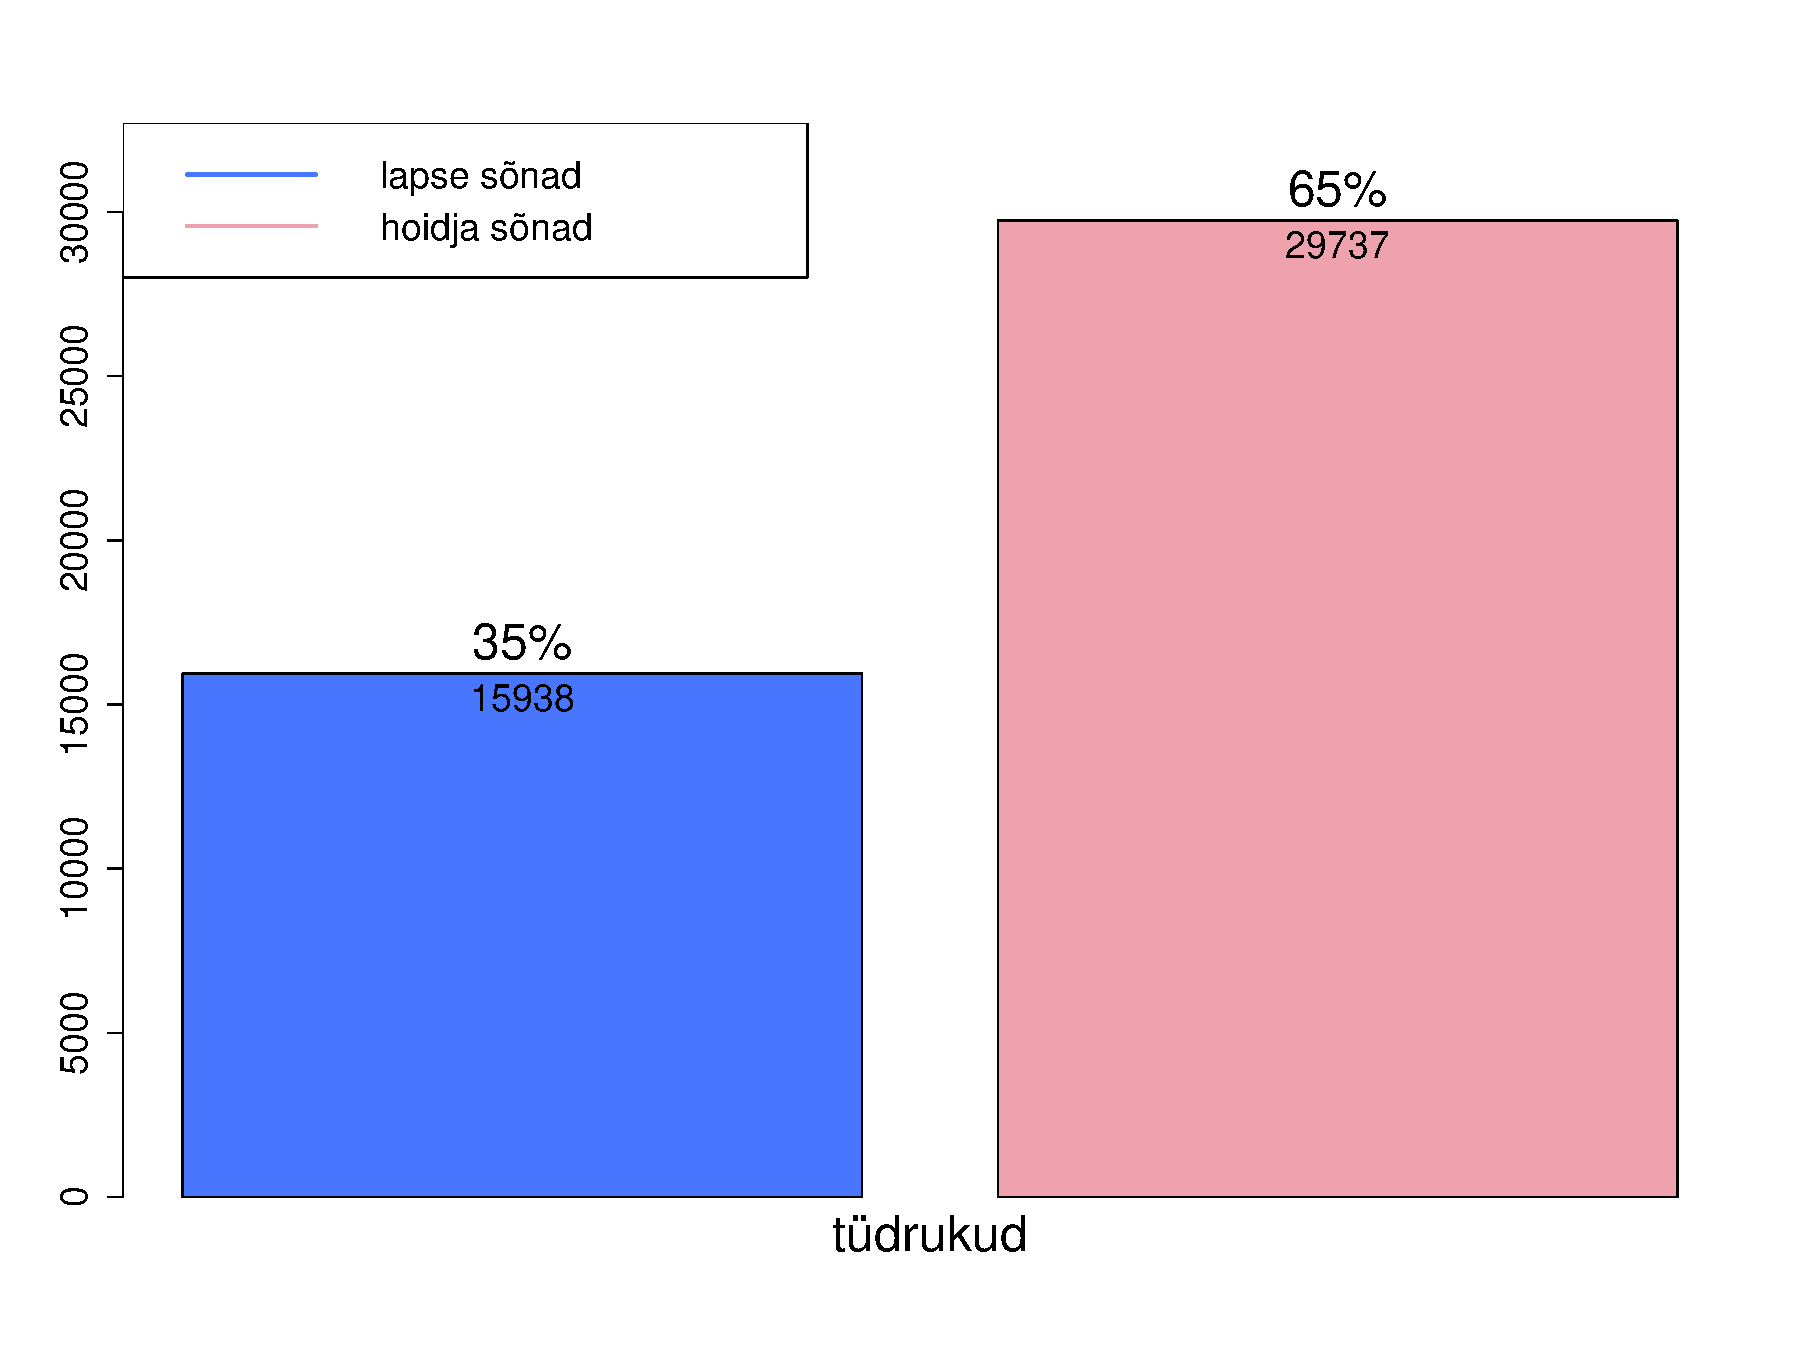
\includegraphics[width=8cm, height=8cm]{kapanen_sugu_sonad}
%     \caption{Kapanen: lapse ja hoidja sõnade sooline jaotumine}
% \end{figure}


\begin{figure}[H]
    \centering
    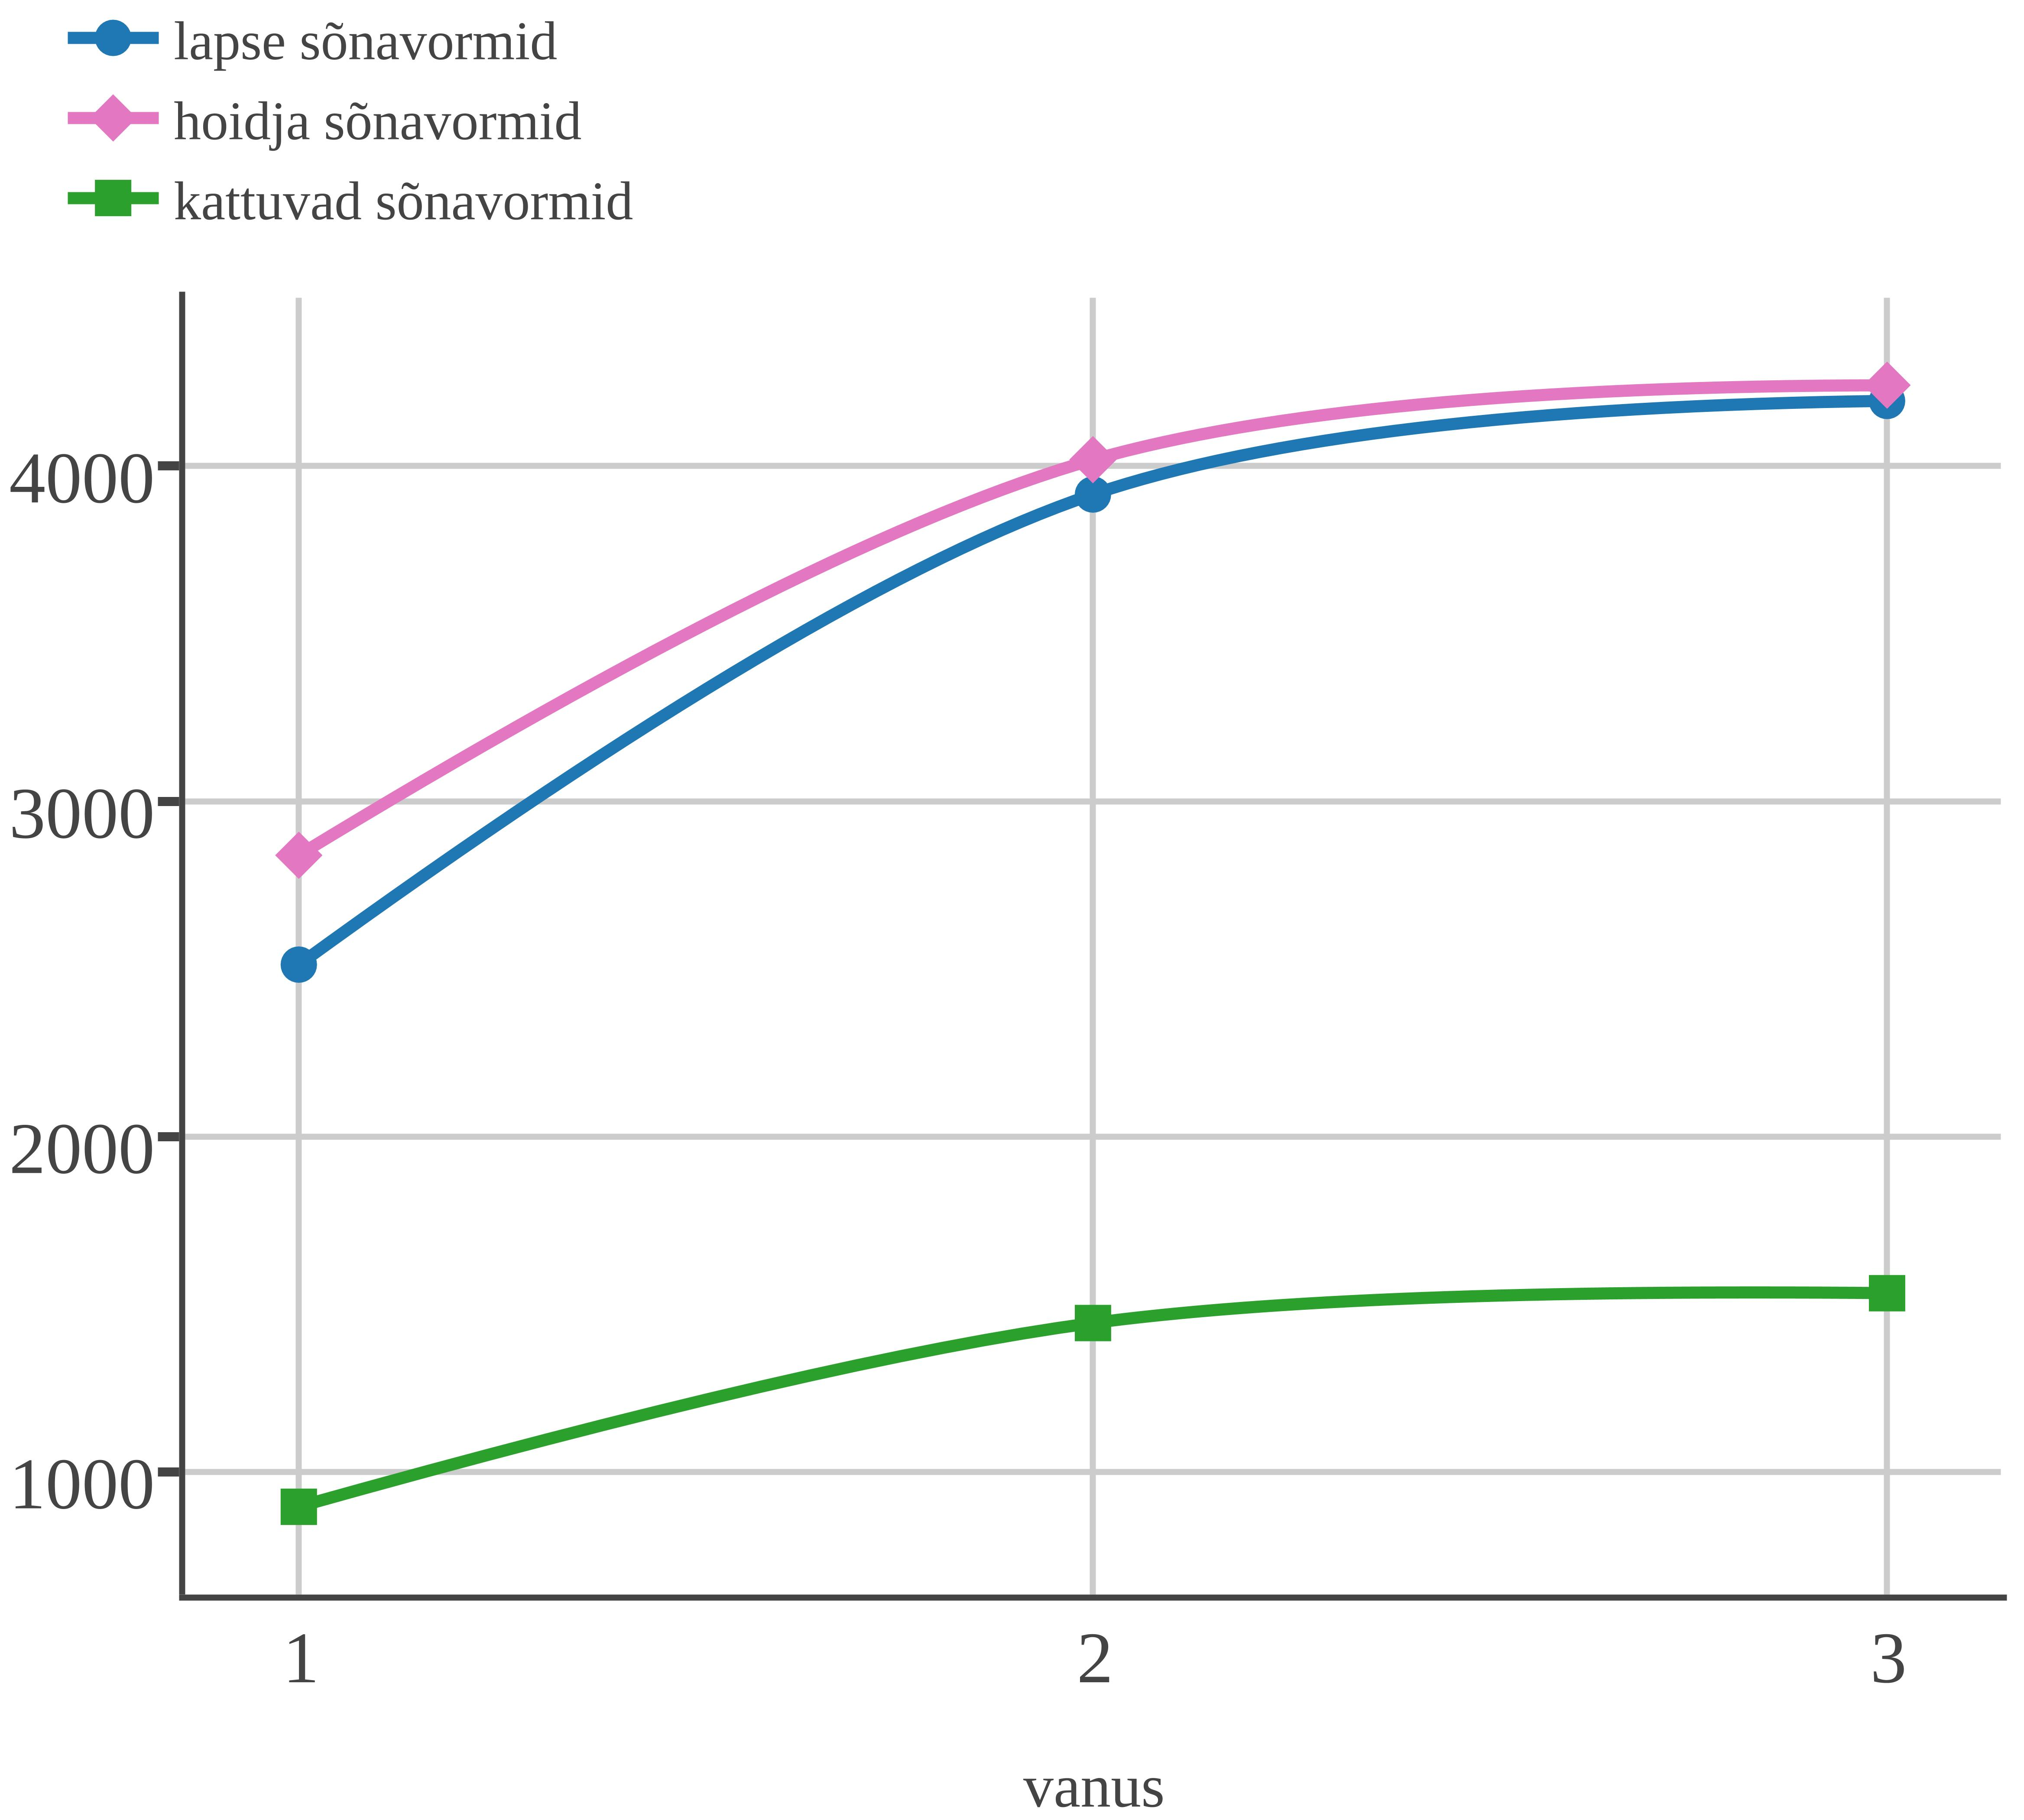
\includegraphics[width=12cm, height=9cm]{kapanen_kum_crop}
    \caption{Kapanen: sõnavormide kasv vanuseliselt}
\end{figure}




\subsubsection{Beek}

Joonisel 8 on kujutatud lapse ja hoidja sõnade vanuselist jaotumist. Kõigis vanusegruppides on hoidja keele sõnad ülekaalus. 0-aastaste laste seas on hoidja sõnu 89\% ja lapse sõnu 11\%. 1-aastaste seas on hoidja sõnu 90\% ja lapse sõnu vaid 10\%. 2-aastaste seas kahaneb hoidja sõnade (78\%) ja suureneb lapse sõnade osakaal (22\%).

\begin{figure}[H]
    \centering
    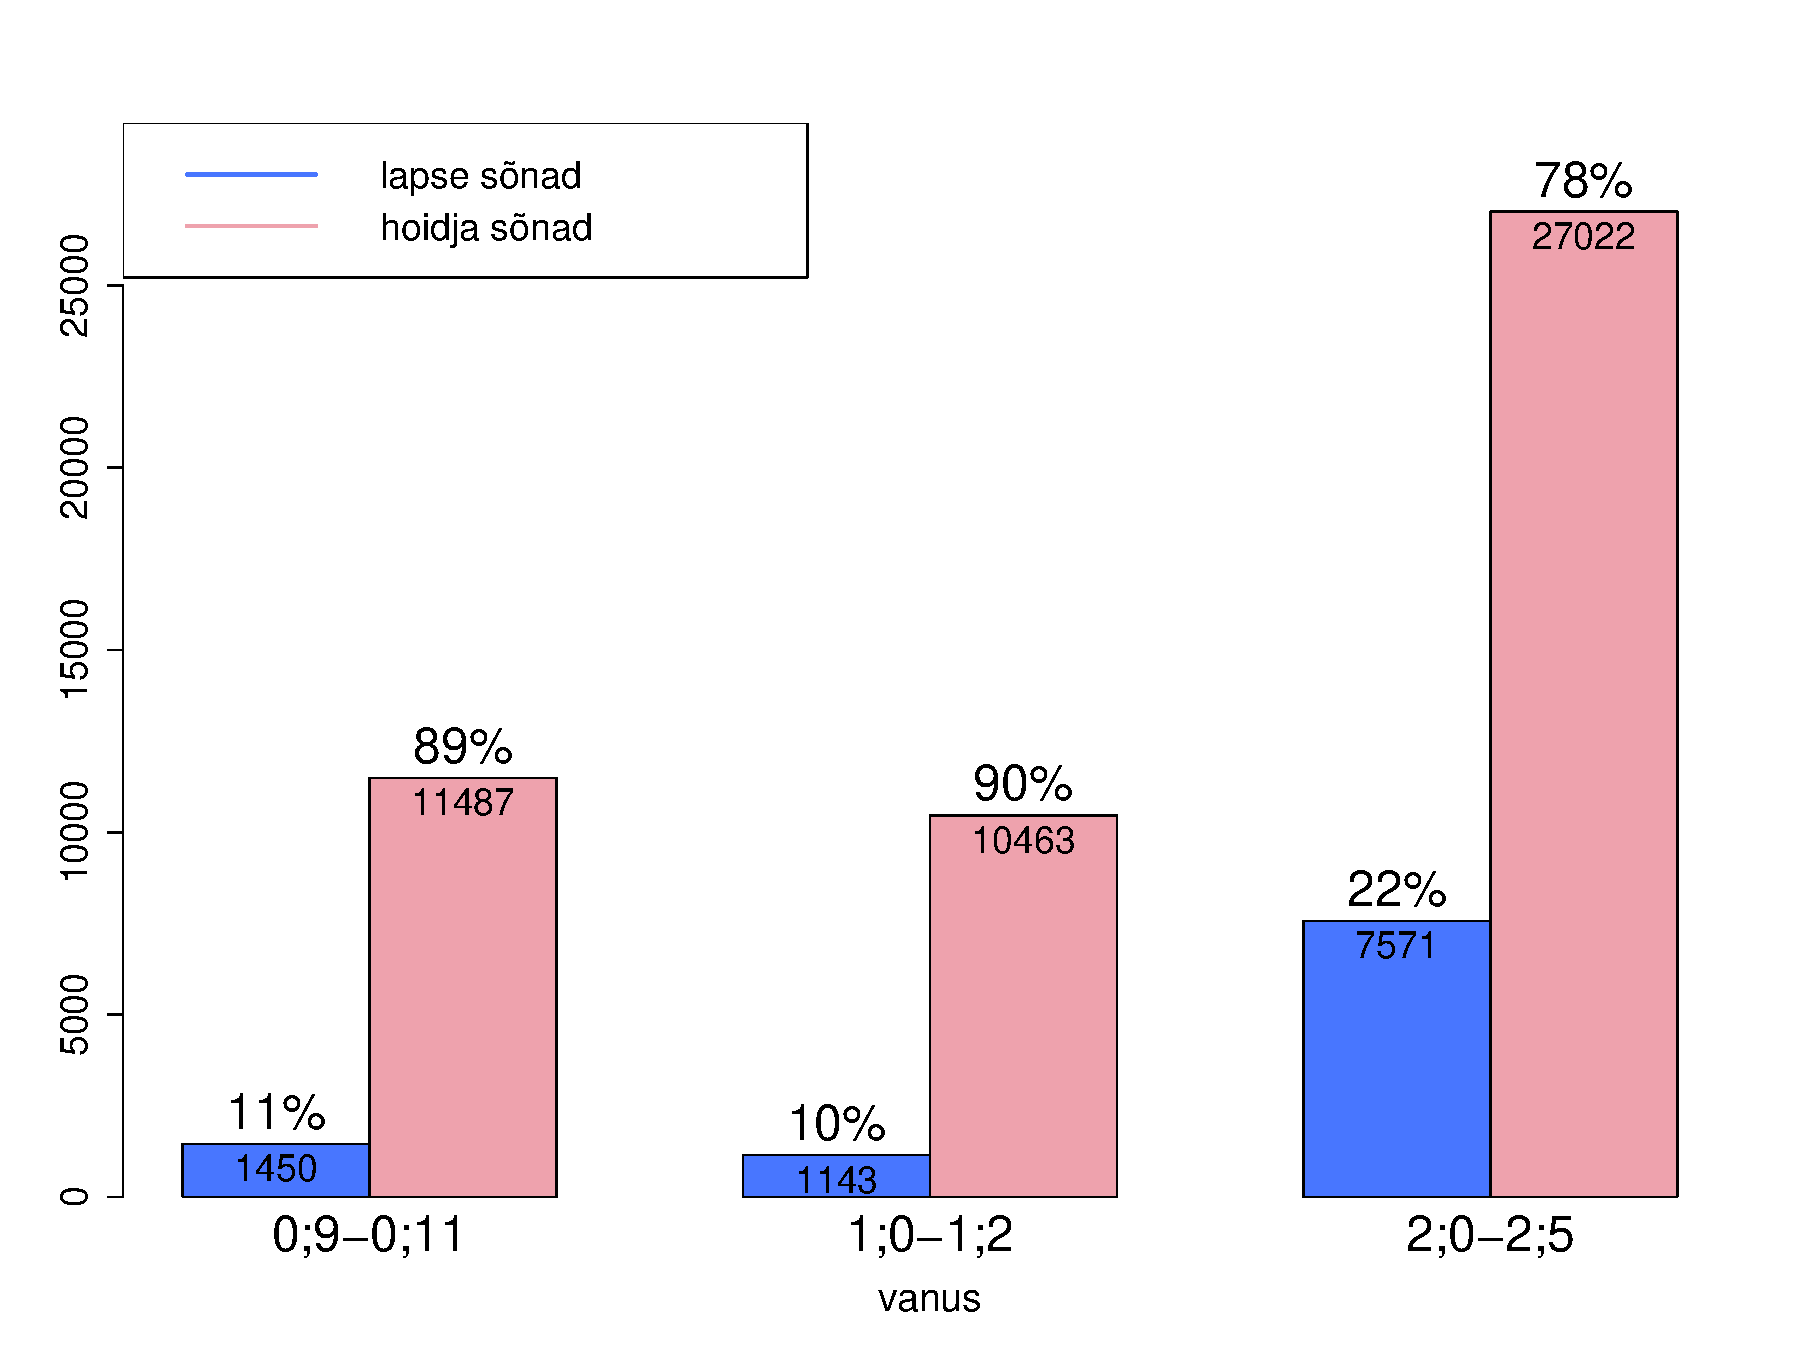
\includegraphics[width=12cm]{beek_vanus_sonad}
    \caption{Beek: lapse ja hoidja sõnade vanuseline jaotumine}
\end{figure}

% \begin{figure}[H]
%     \centering
%     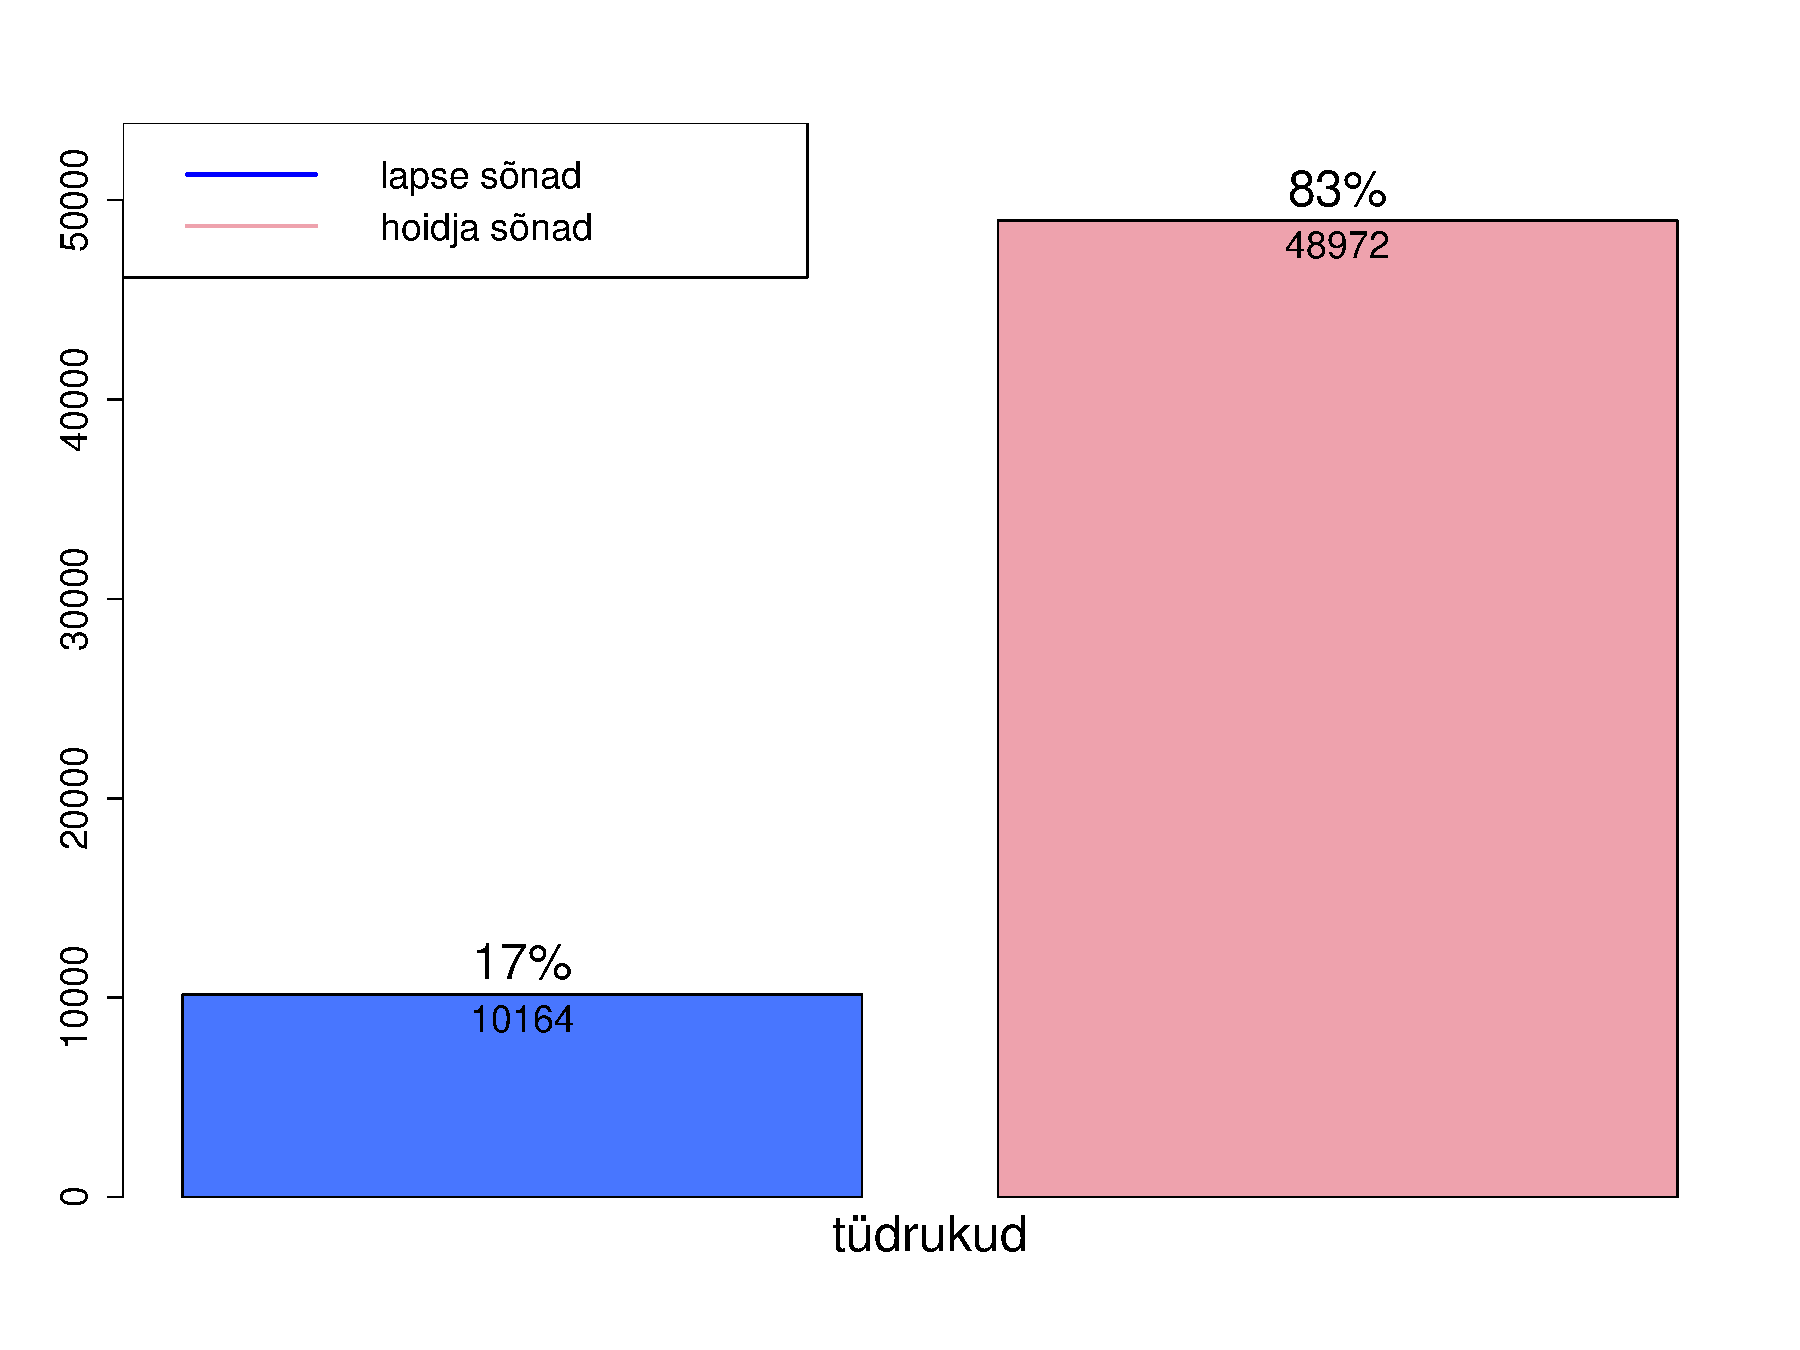
\includegraphics[width=11cm, height=9cm]{beek_sugu_sonad}
%     \caption{Beek: lapse ja hoidja sõnade sooline jaotumine}
% \end{figure}


\begin{figure}[H]
    \centering
    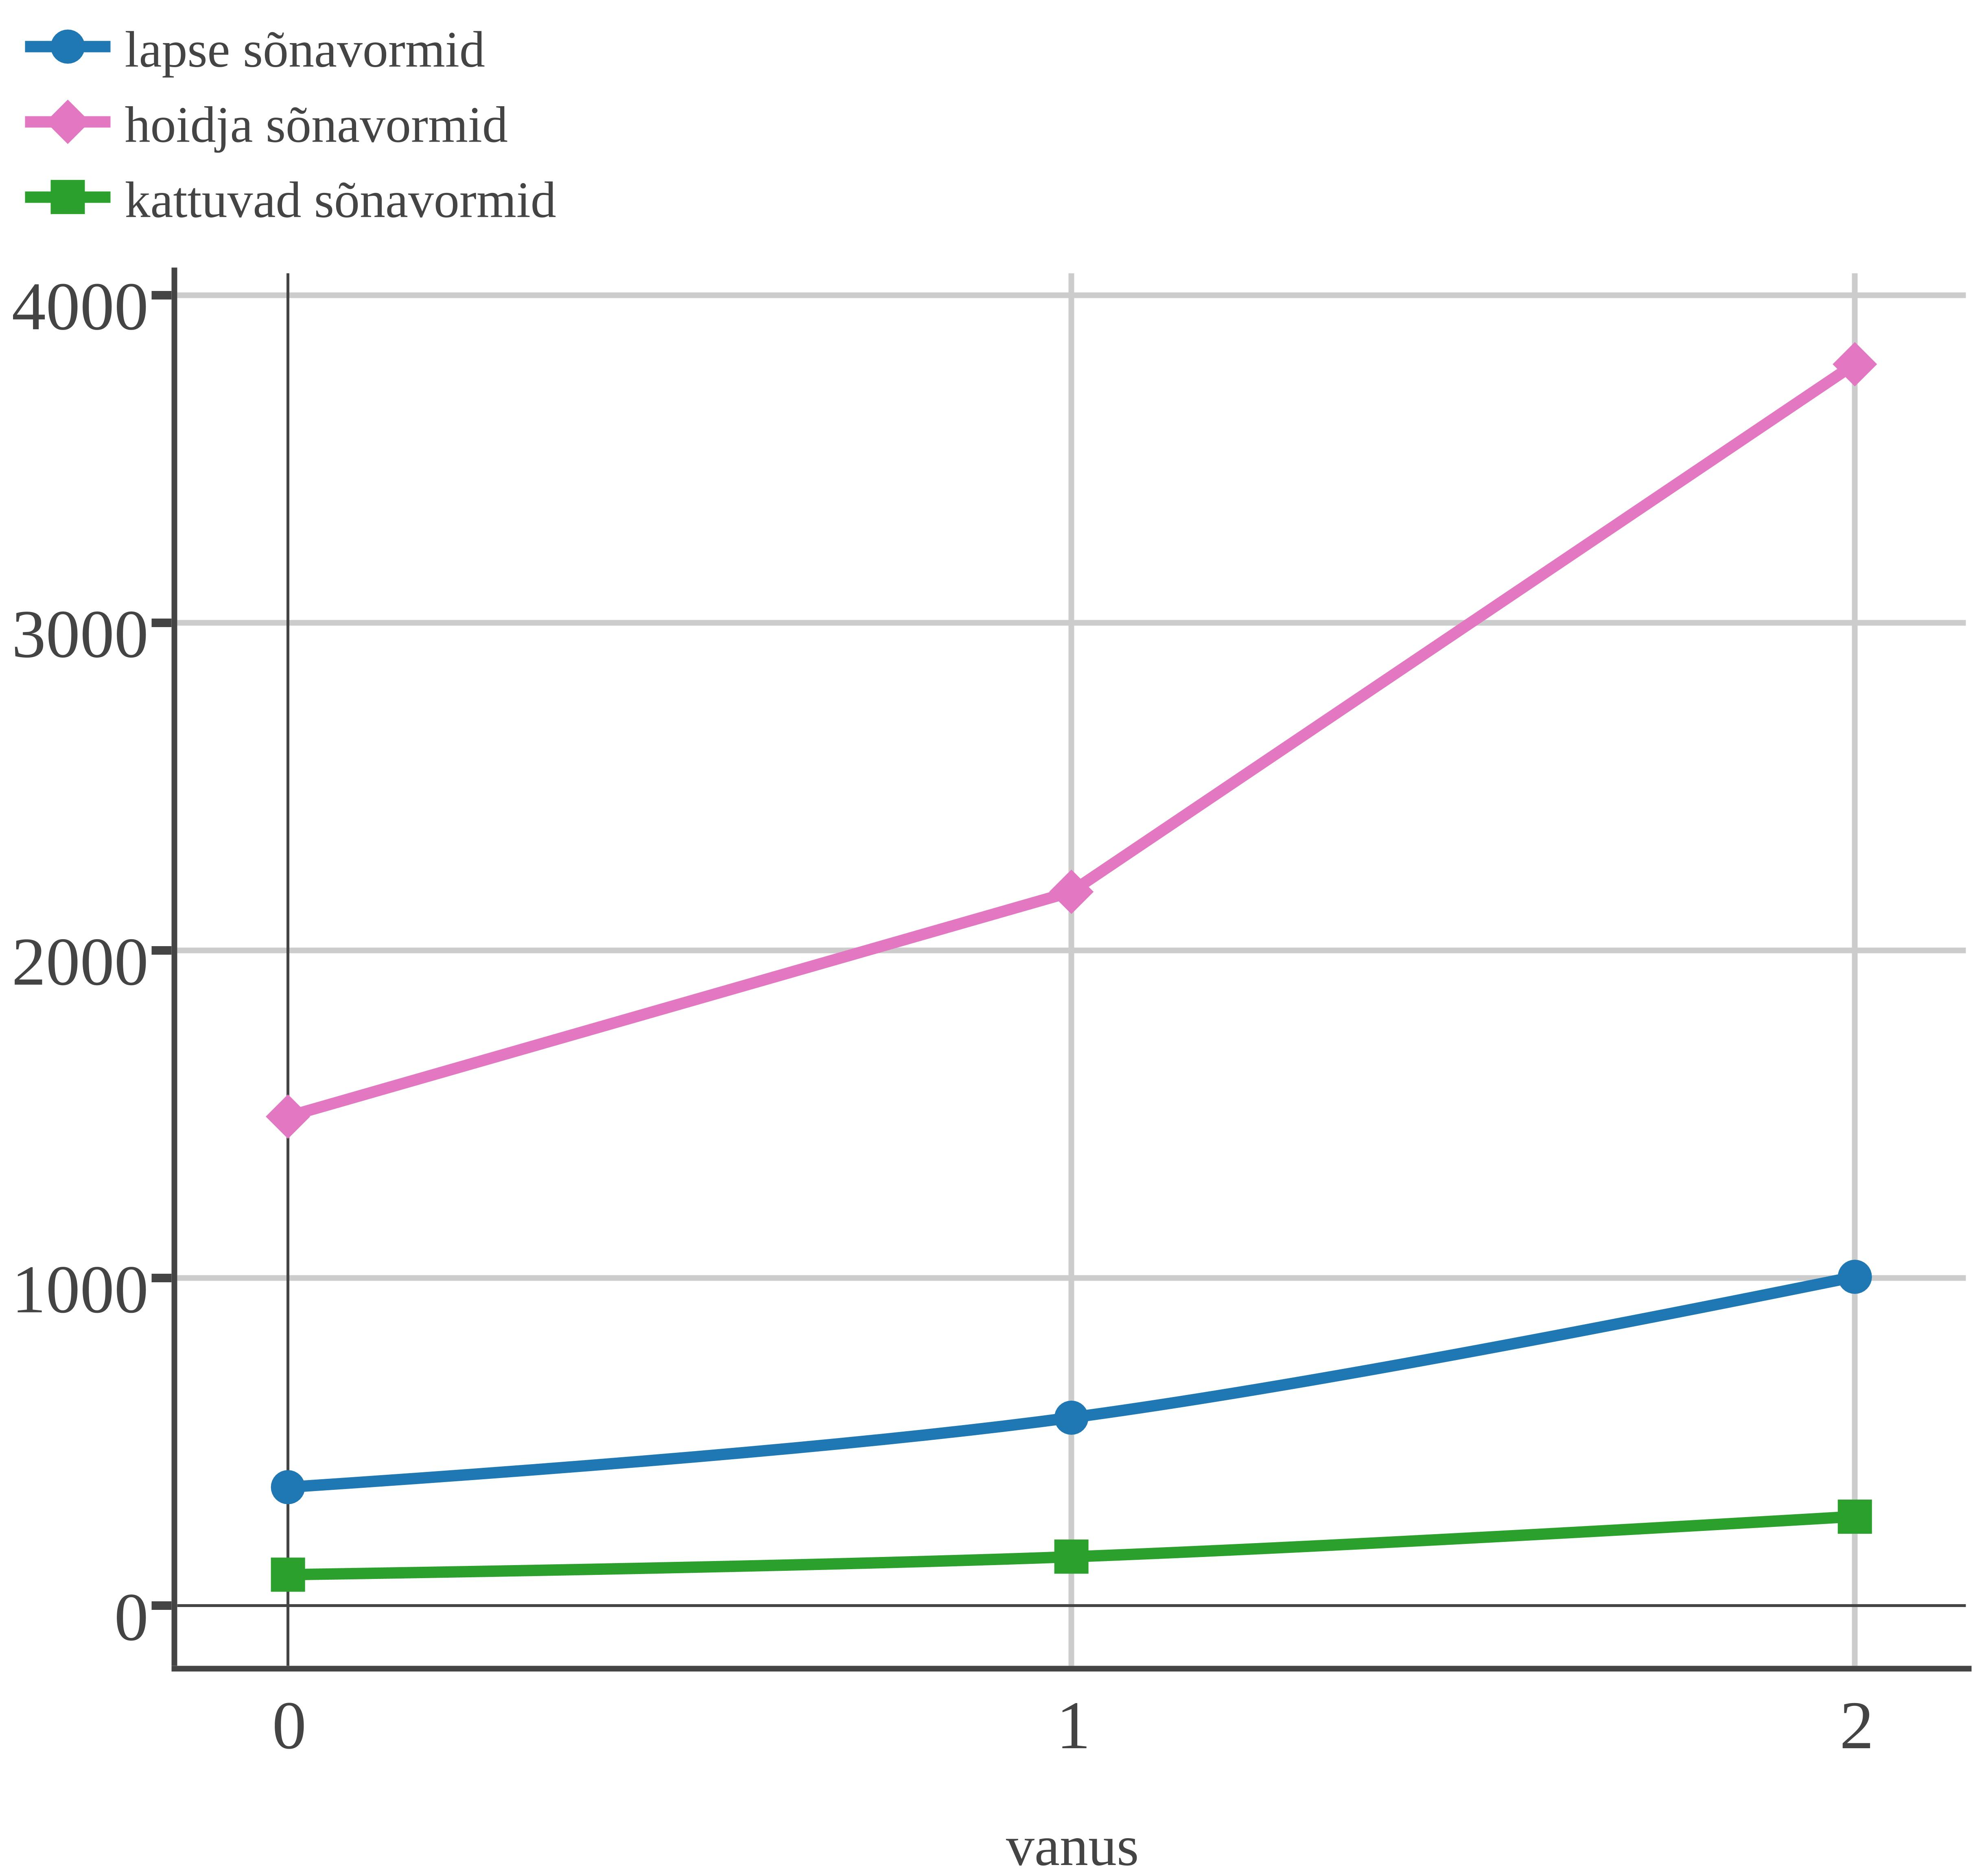
\includegraphics[width=12cm, height=9cm]{beek_kum_crop}
    \caption{Beek: sõnavormide kasv vanuseliselt}
\end{figure}




\subsubsection{Kohler}

Joonisel 10 on kujutatud lapse ja hoidja sõnade vanuselist jaotumist. Kõigis vanusegruppides on hoidja keele sõnad ülekaalus. 0-aastaste laste seas on hoidja sõnu lausa 98\% ja lapse sõnu vaid 2\%. 1-aastaste seas on hoidja sõnu 89\% ja lapse sõnu vaid 11\%. 2-aastaste seas kahaneb hoidja sõnade (78\%) ja suureneb lapse sõnade osakaal (22\%).

\begin{figure}[H]
    \centering
    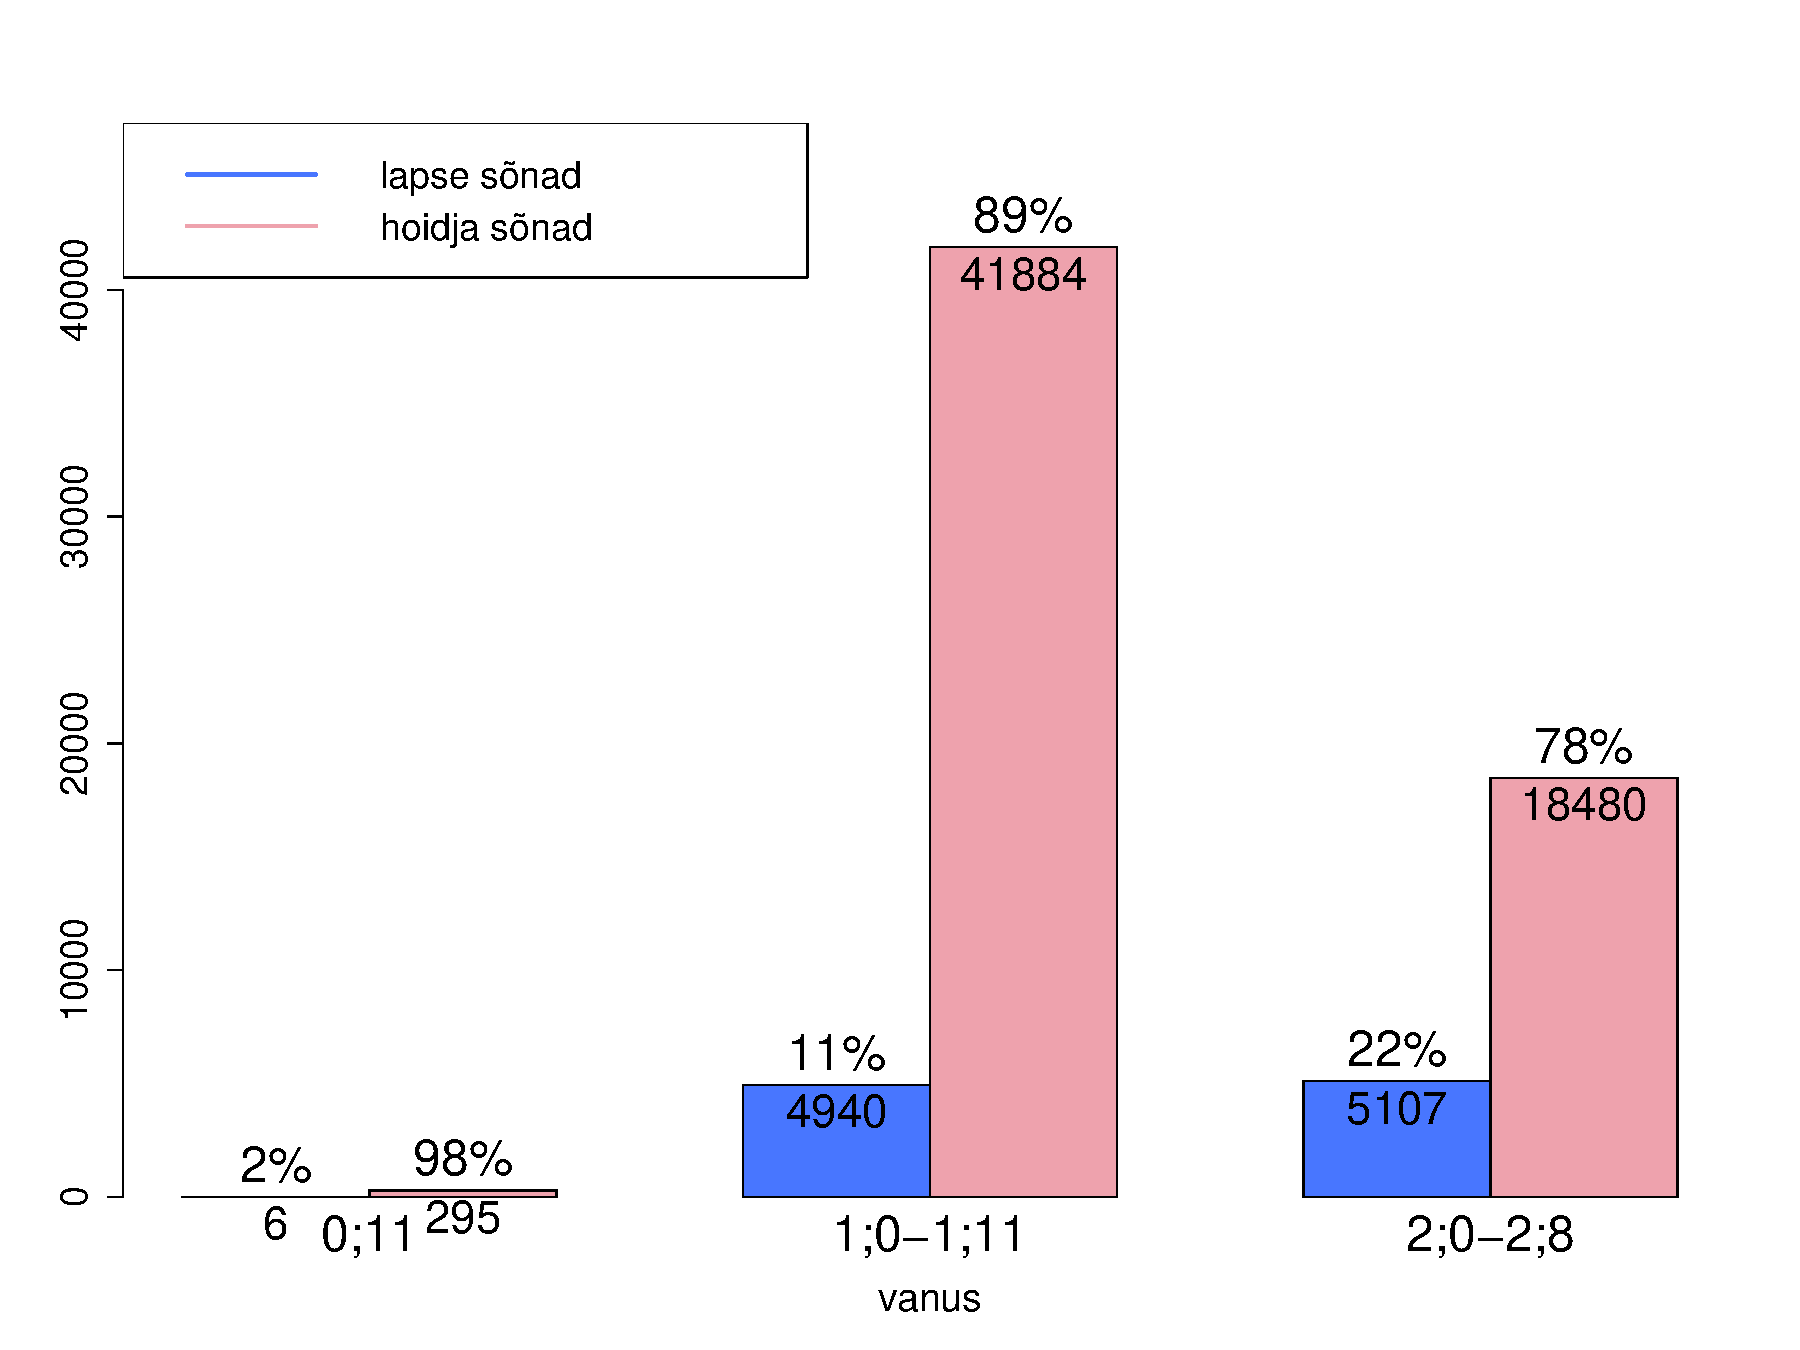
\includegraphics[width=12cm, height=9cm]{kohler_vanus_sonad}
    \caption{Kohler: lapse ja hoidja sõnade vanuseline jaotumine}
\end{figure}

Joonis 11 kujutab lapse ja hoidja sõnade soolist jaotumist. Nii tüdrukute kui ka poiste seas on hoidja ja lapse sõnade jaotumine ühtlane. Tüdrukute seas on hoidja sõnade osakaal 87\% ja poiste seas 85\%. Lapse sõnade osakaal tüdrukute seas on 13\% ja poiste seas 15\%.

\begin{figure}[H]
    \centering
    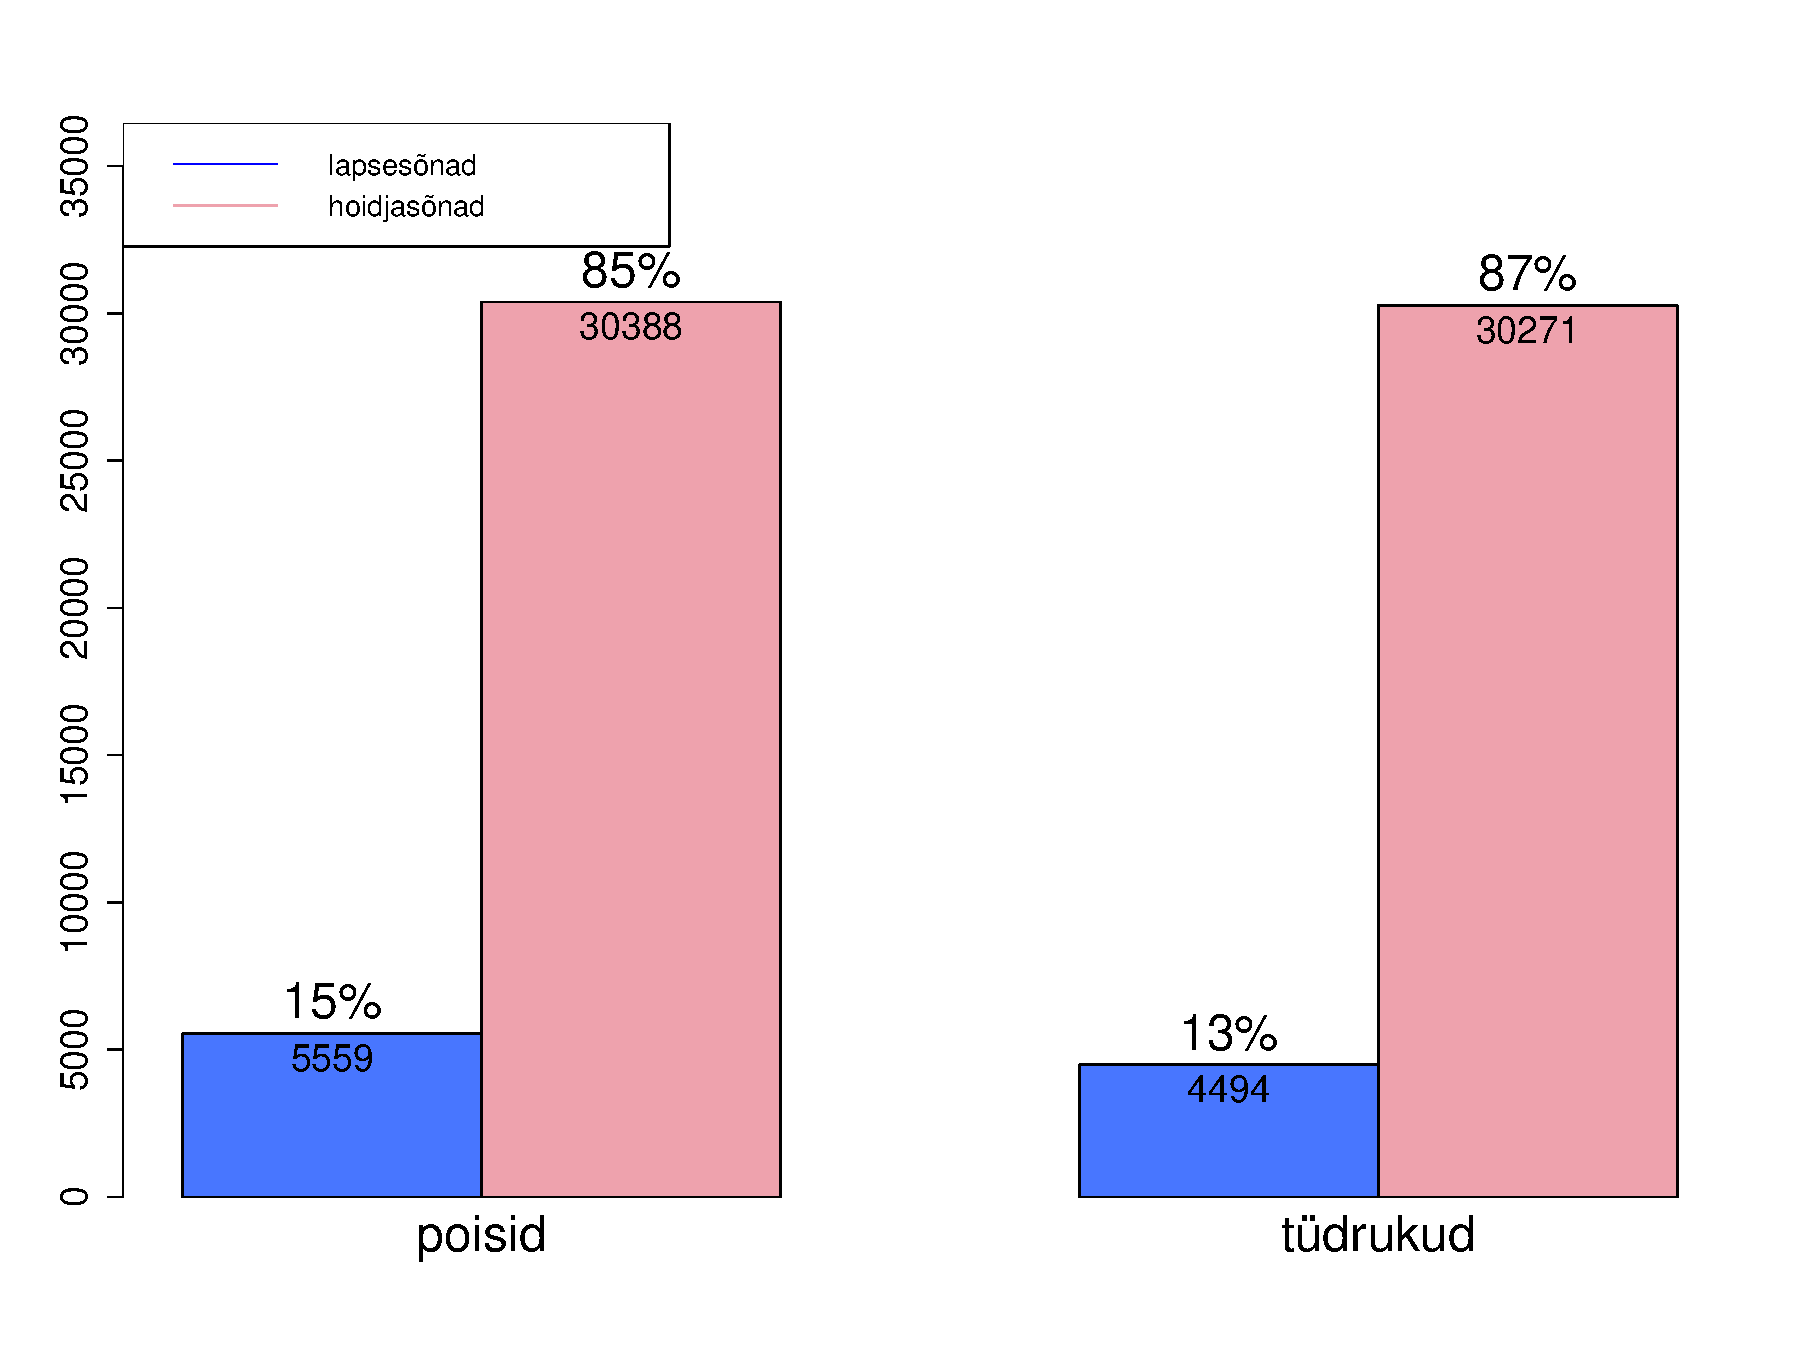
\includegraphics[width=12cm, height=10cm]{kohler_sugu_sonad}
    \caption{Kohler: lapse ja hoidja sõnade sooline jaotumine}
\end{figure}

\begin{figure}[H]
    \centering
    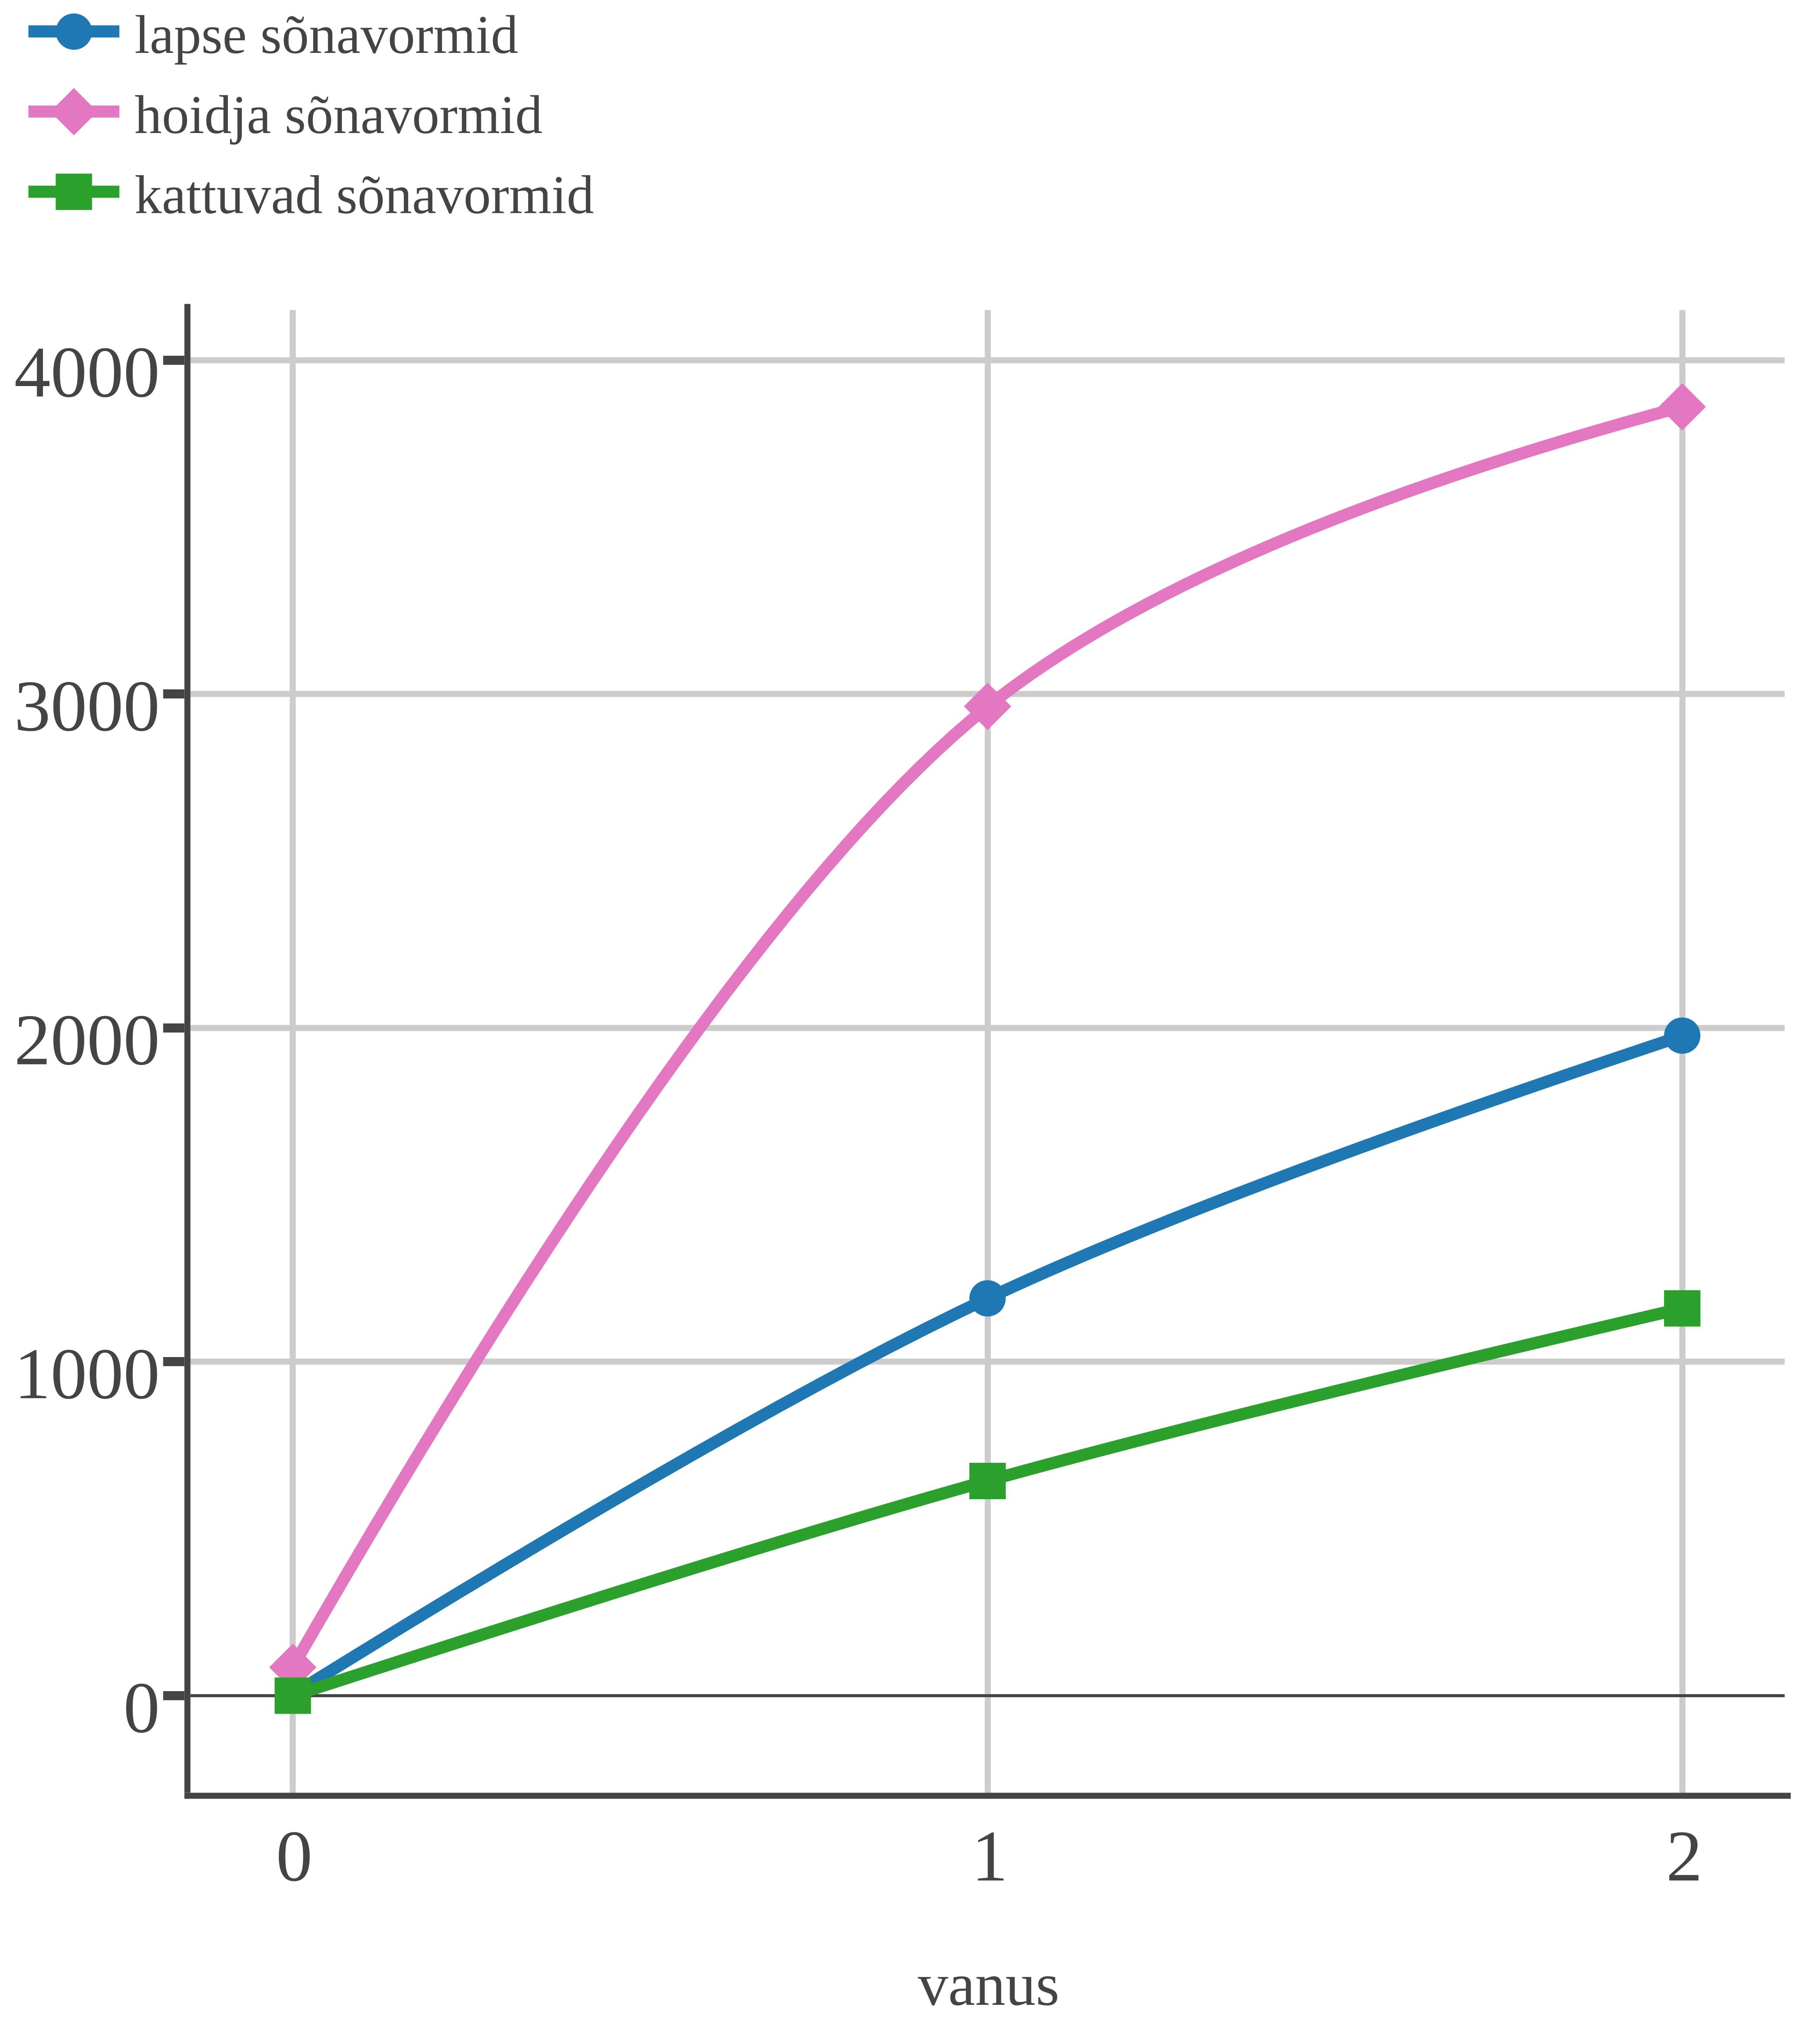
\includegraphics[width=12cm, height=9cm]{kohler_kum_crop}
    \caption{Kohler: sõnavormide kasv vanuseliselt}
\end{figure}

\begin{figure}[H]
    \centering
    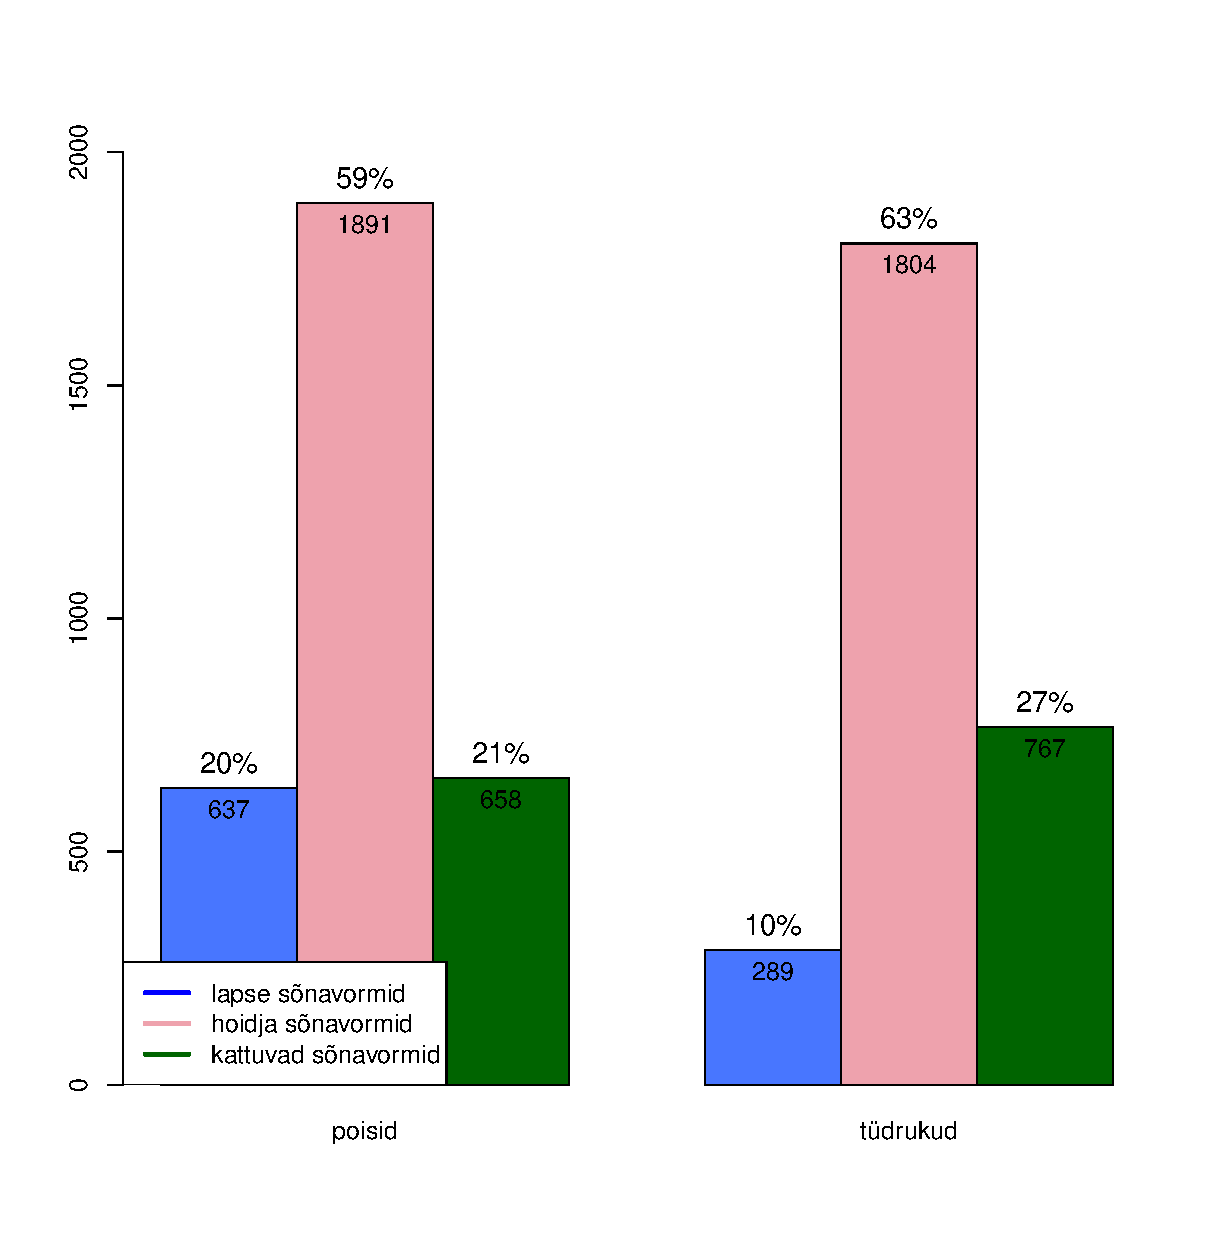
\includegraphics[width=11cm, height=9cm]{kohler_sonavormid_sugu}
    \caption{Kohler: sõnavormide sooline jaotumine}
\end{figure}


\subsubsection{Vija}

Joonisel 14 on kujutatud lapse ja hoidja sõnade vanuselist jaotumist. Valdavalt kõigis vanusegruppides on hoidja keele sõnad ülekaalus, v.a. 3-aastased. 1-aastaste laste seas on hoidja sõnade osakaal 75\% ja lapse sõnad 25\%. Vanuse suurenedes suureneb ka lapse sõnade osakaal ja väheneb hoidja sõnade osakaal. 2-aastaste seas on hoidja sõnade hulk 59\% ja lapse sõnu 41\%. 3-aastaste laste seas on hoidja sõnu vähem kui lapse sõnu (42\% vs 58\%).

\begin{figure}[H]
    \centering
    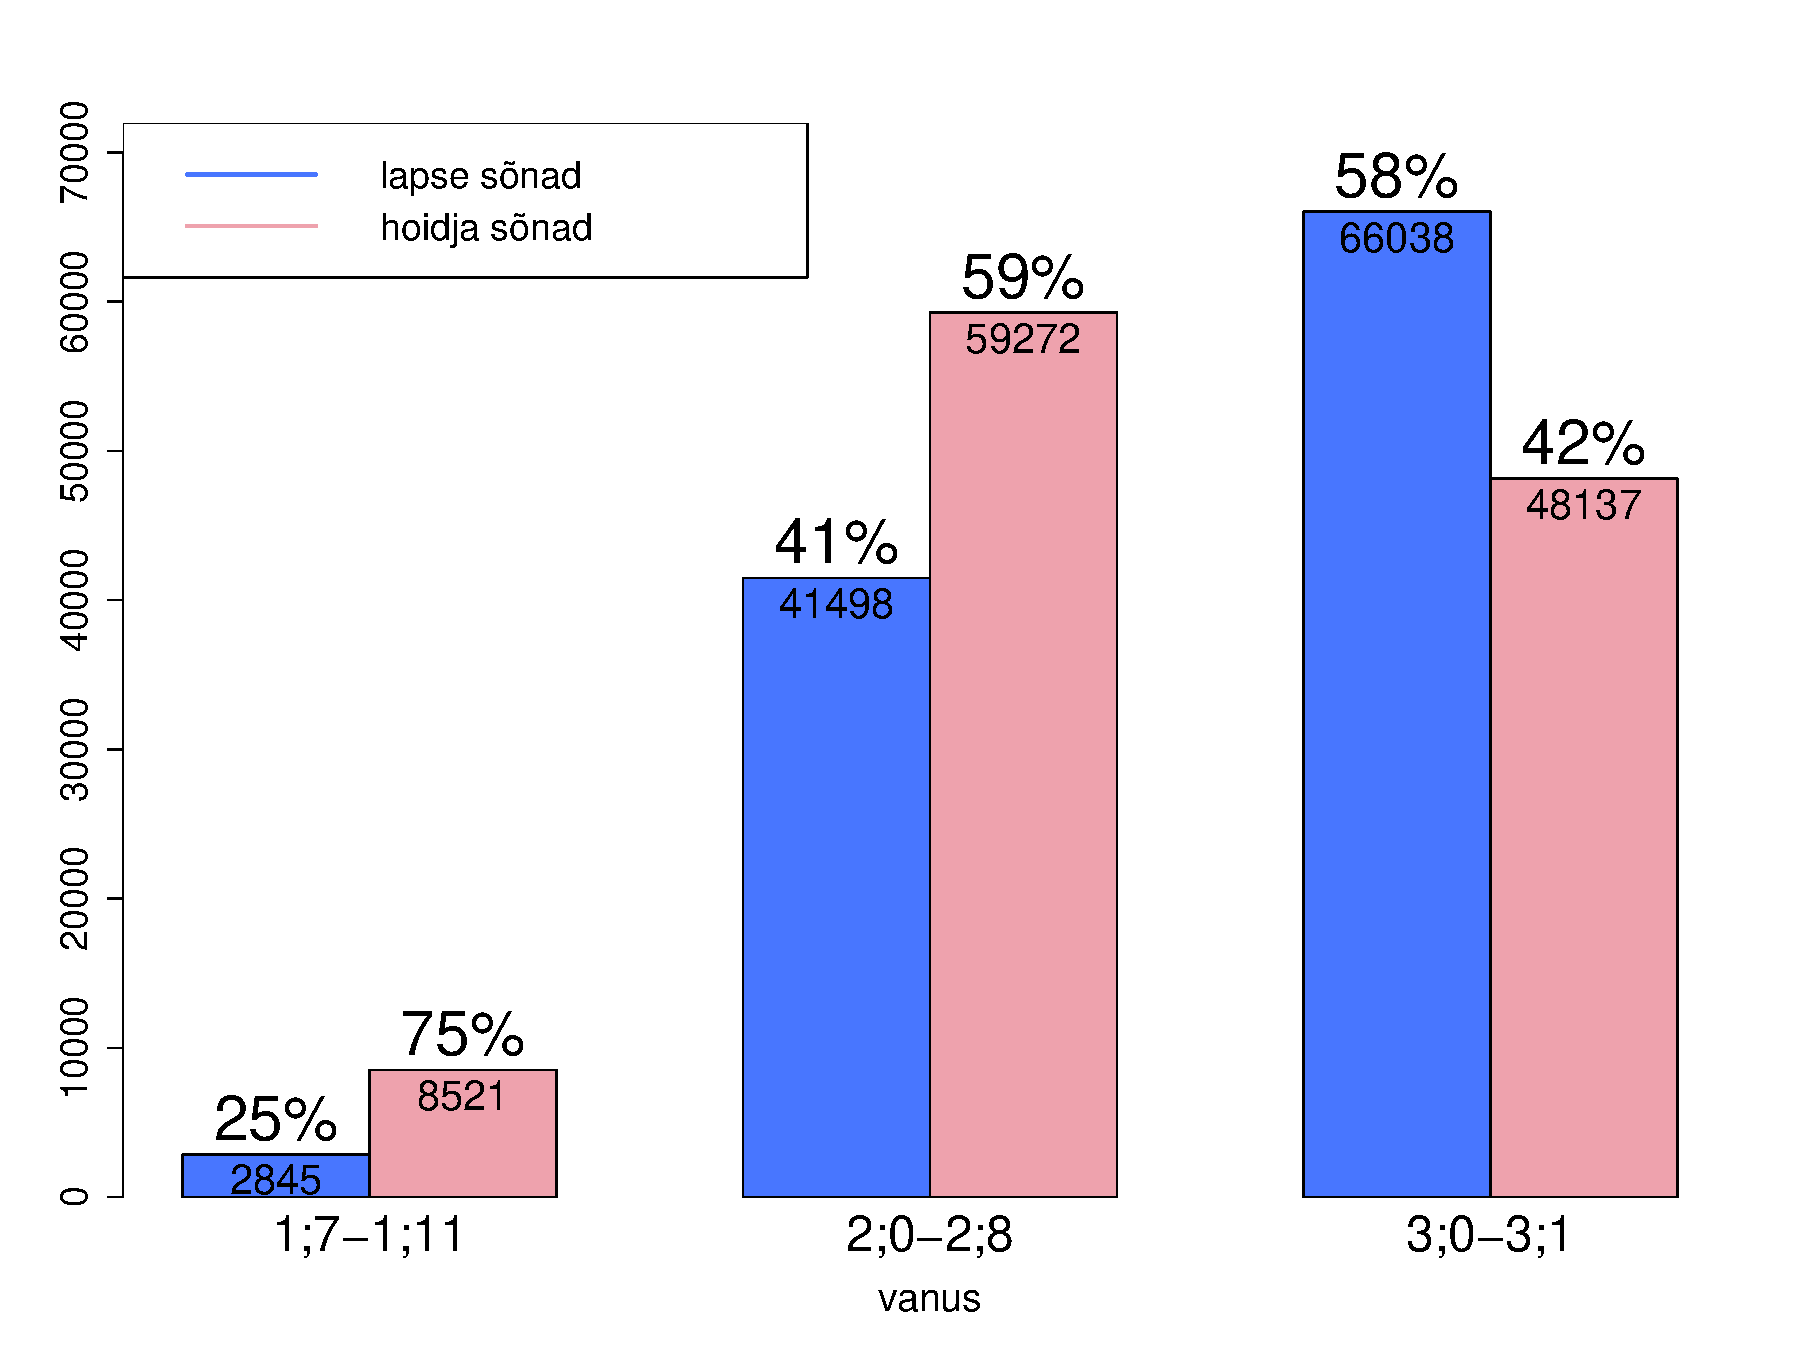
\includegraphics[width=12cm, height=9cm]{vija_vanus_sonad}
    \caption{Vija: lapse ja hoidja sõnade vanuseline jaotumine}
\end{figure}

% \begin{figure}[H]
%     \centering
%     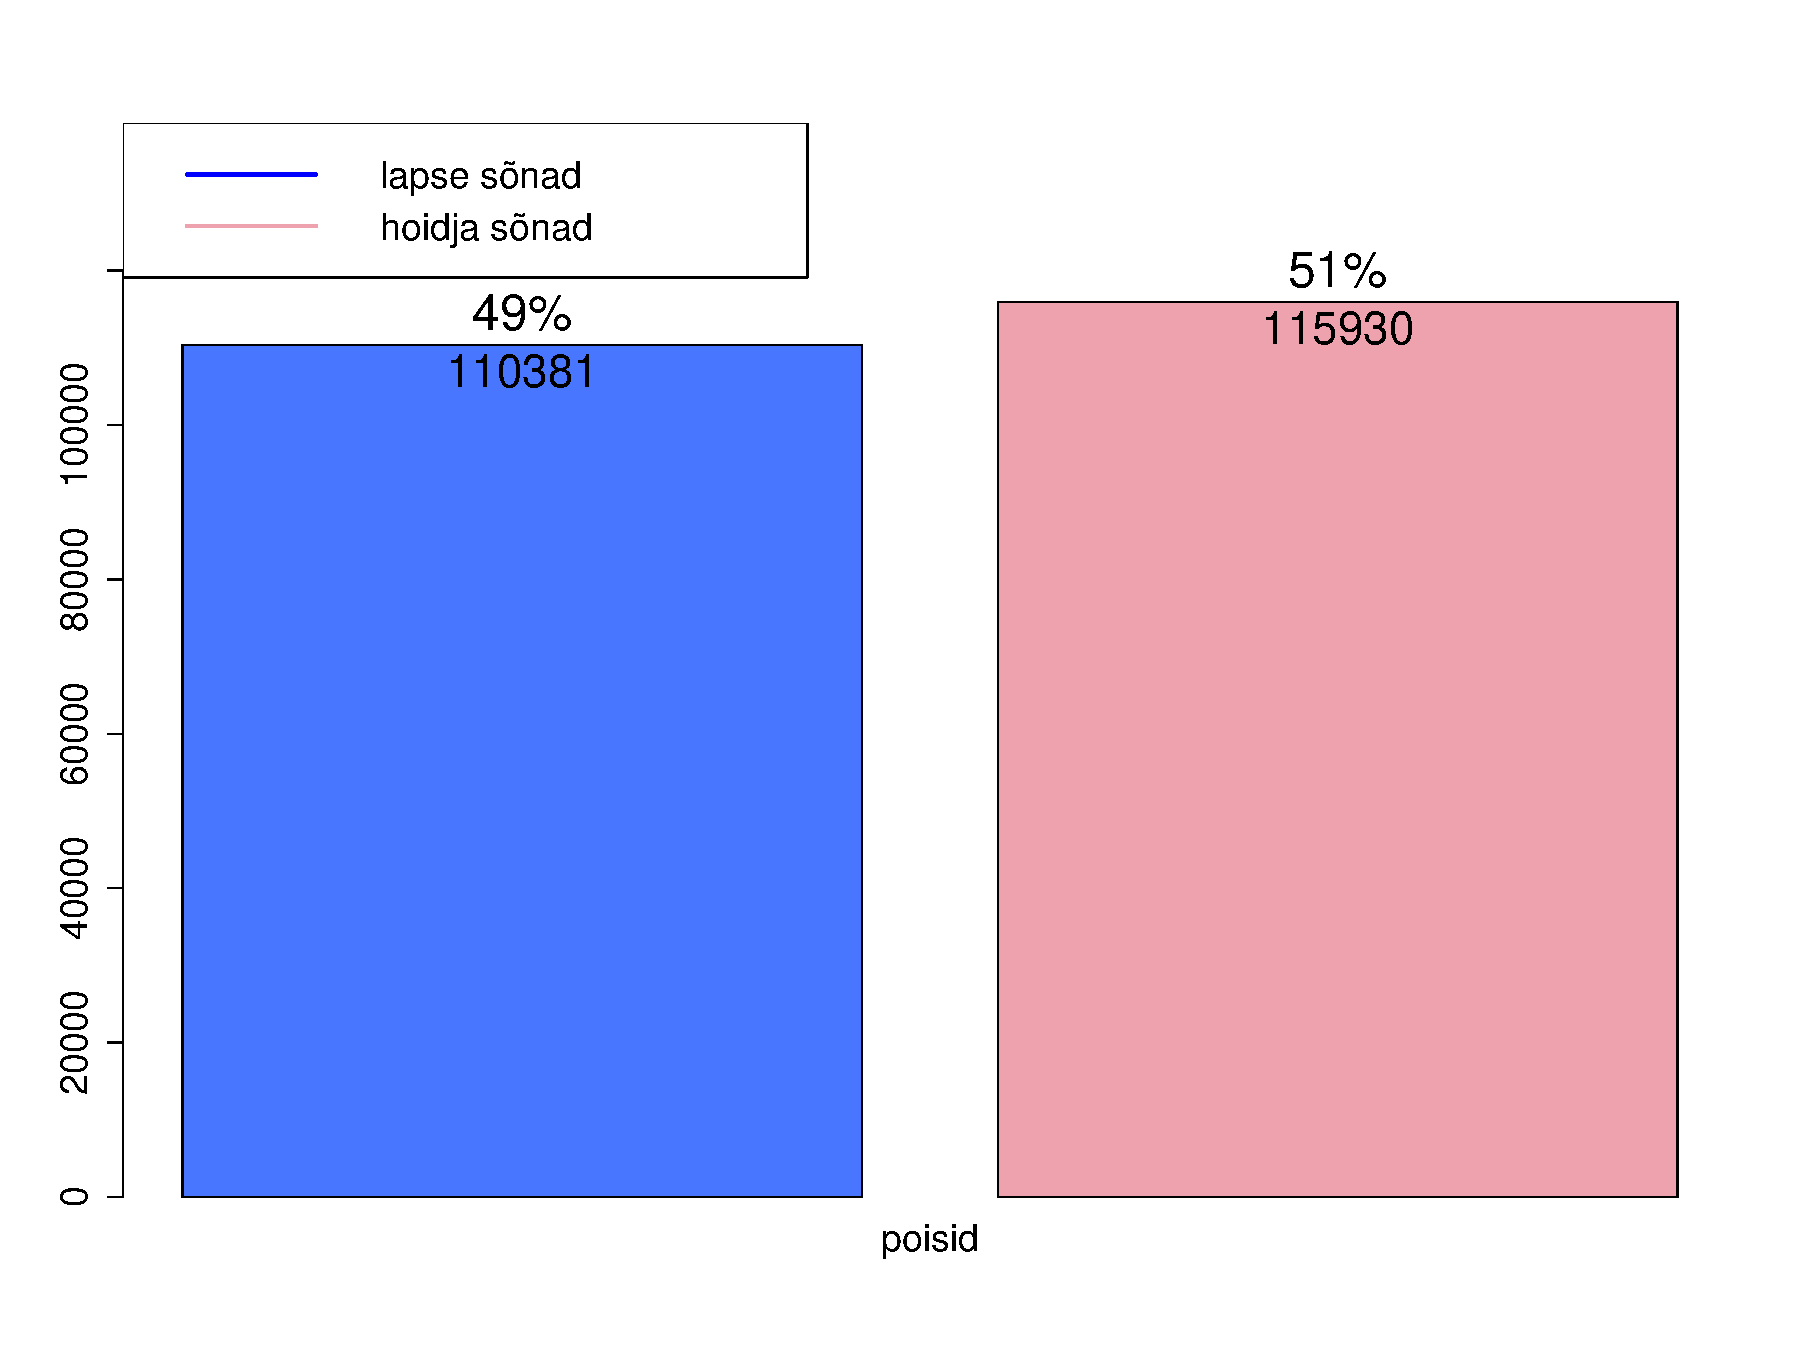
\includegraphics[width=11cm, height=9cm]{vija_sugu_sonad}
%     \caption{Vija: lapse ja hoidja sõnade sooline jaotumine}
% \end{figure}

\begin{figure}[H]
    \centering
    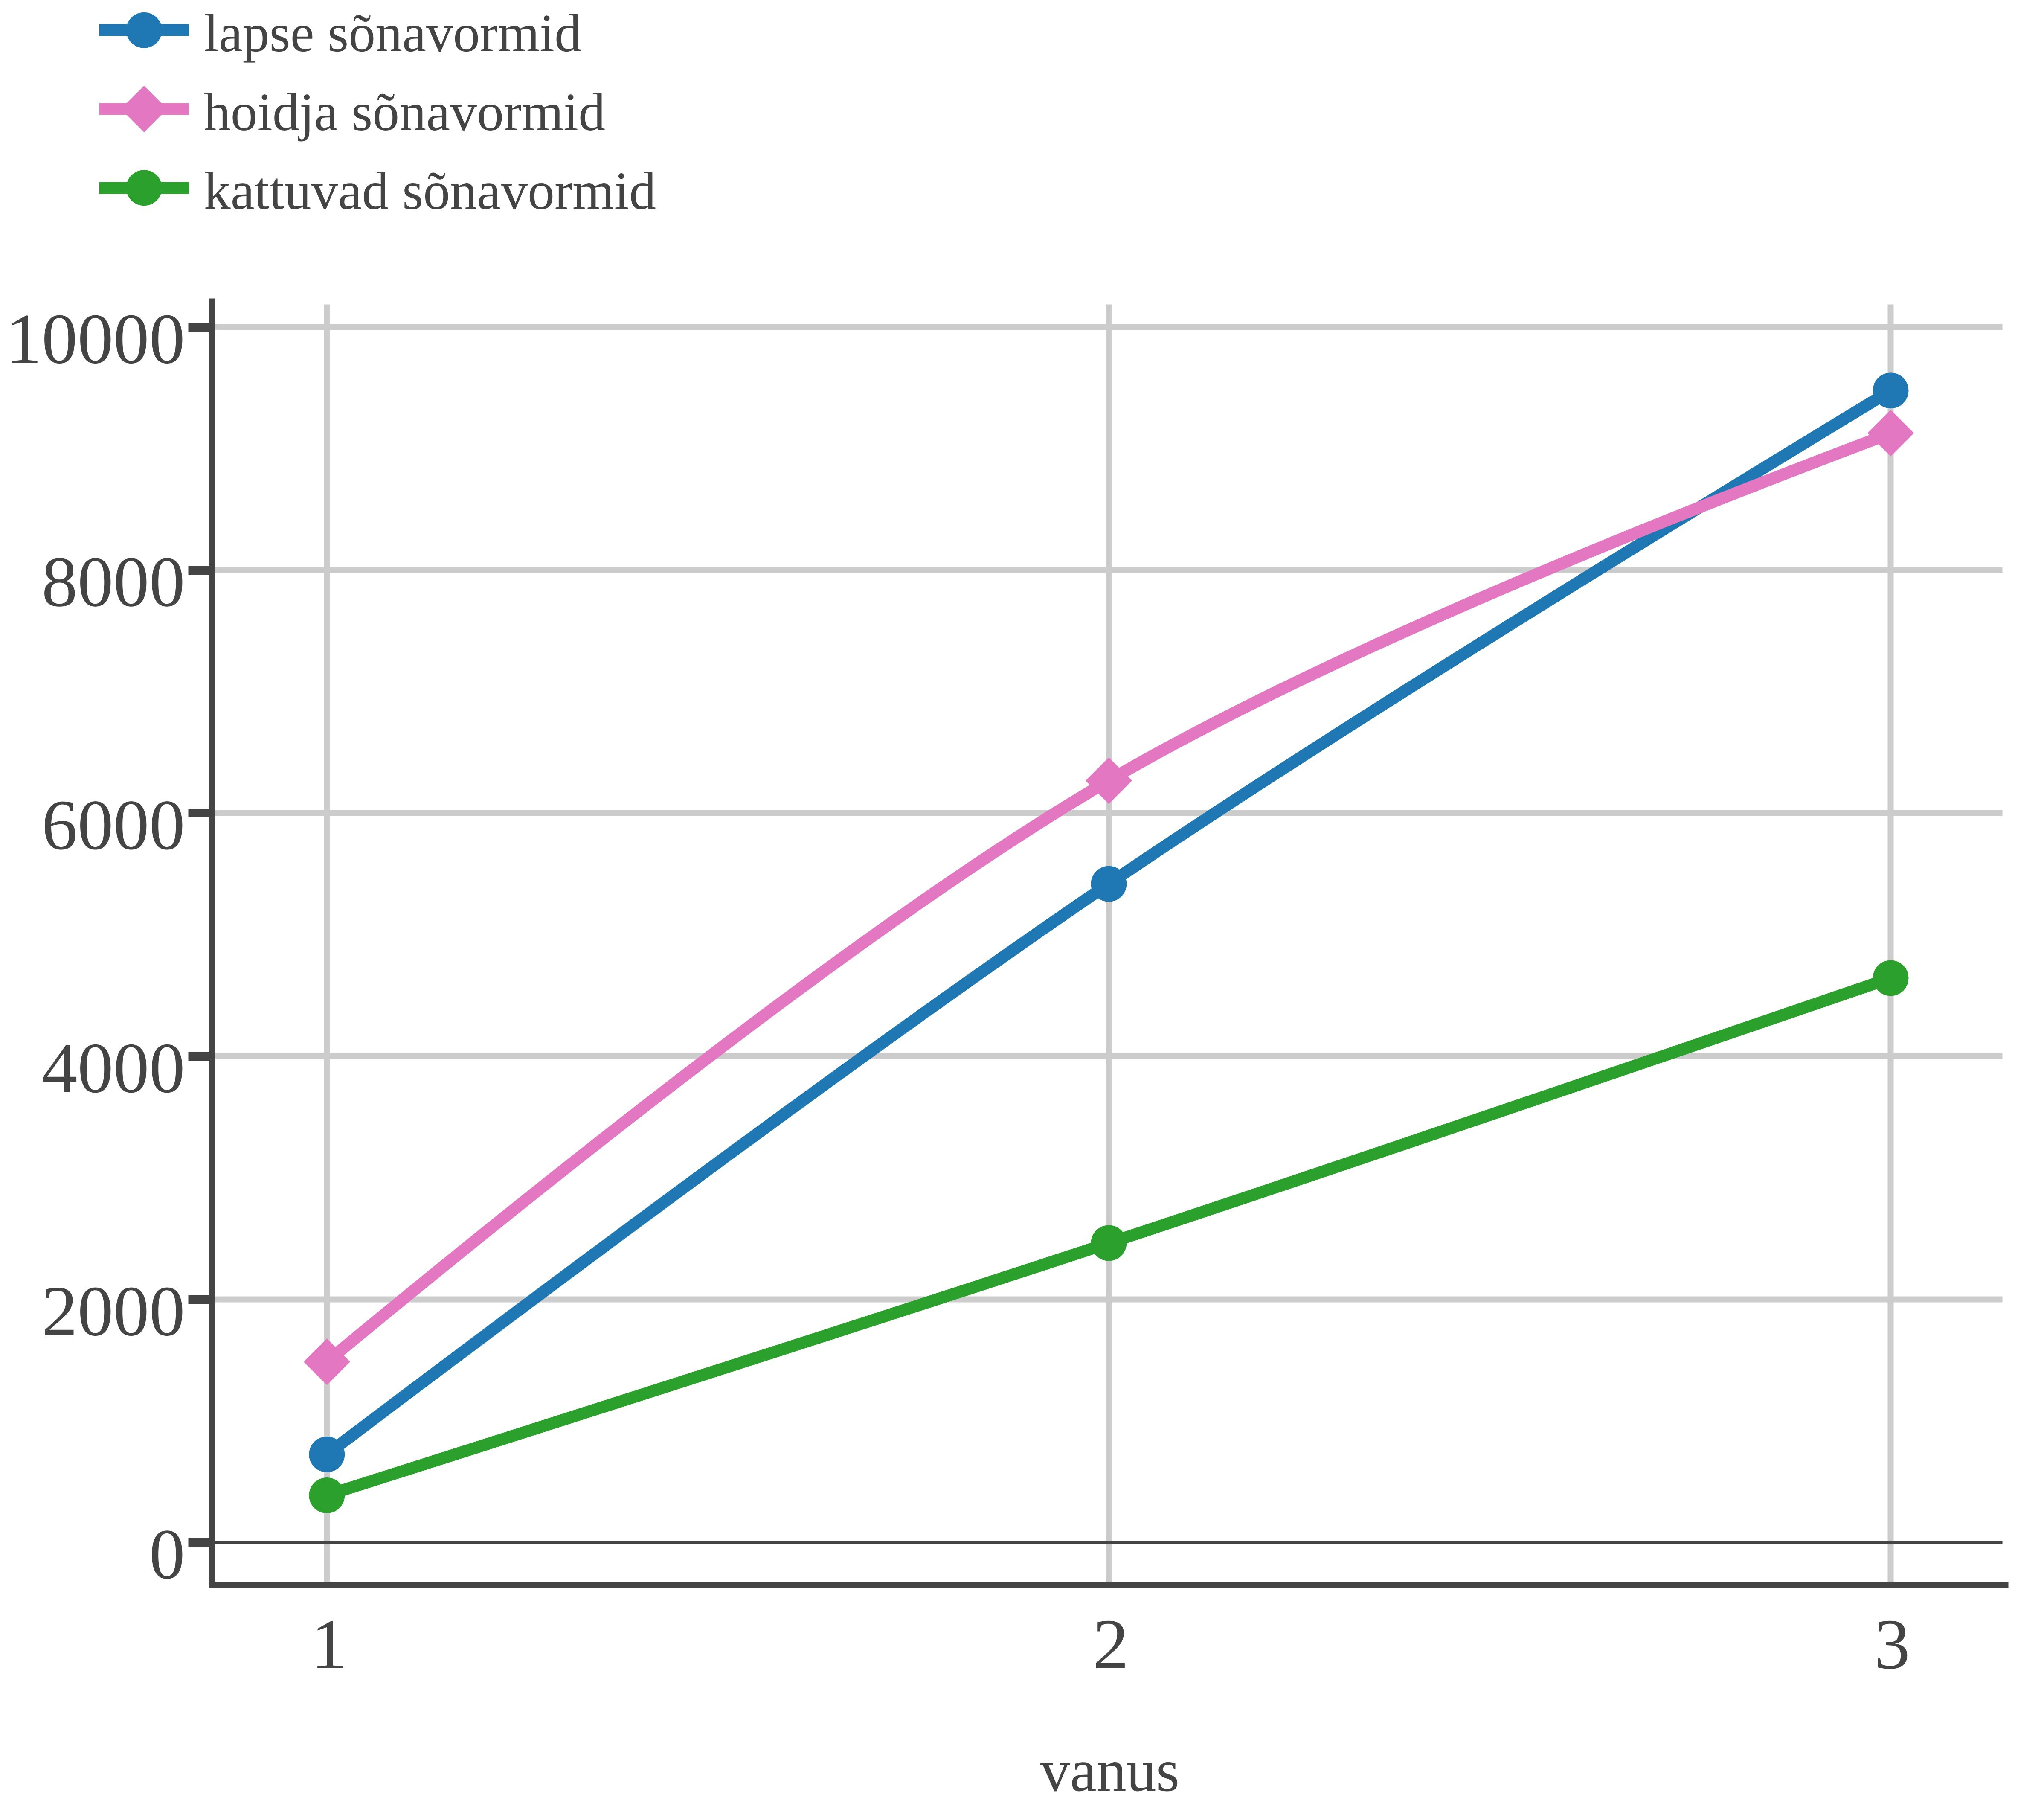
\includegraphics[width=11cm, height=9cm]{vija_kum_crop}
    \caption{Vija: sõnavormide kasv vanuseliselt}
\end{figure}



\subsubsection{Argus}

Joonisel 16 on kujutatud lapse ja hoidja sõnade vanuselist jaotumist. Kõigis vanusegruppides on hoidja keele sõnad ülekaalus. 1-aastaste laste seas on hoidja sõnade osakaal 78\% ja lapse sõnad 22\%. 2-aastaste seas on hoidja sõnade hulk 66\% ja lapse sõnu 34\%.

\begin{figure}[H]
    \centering
    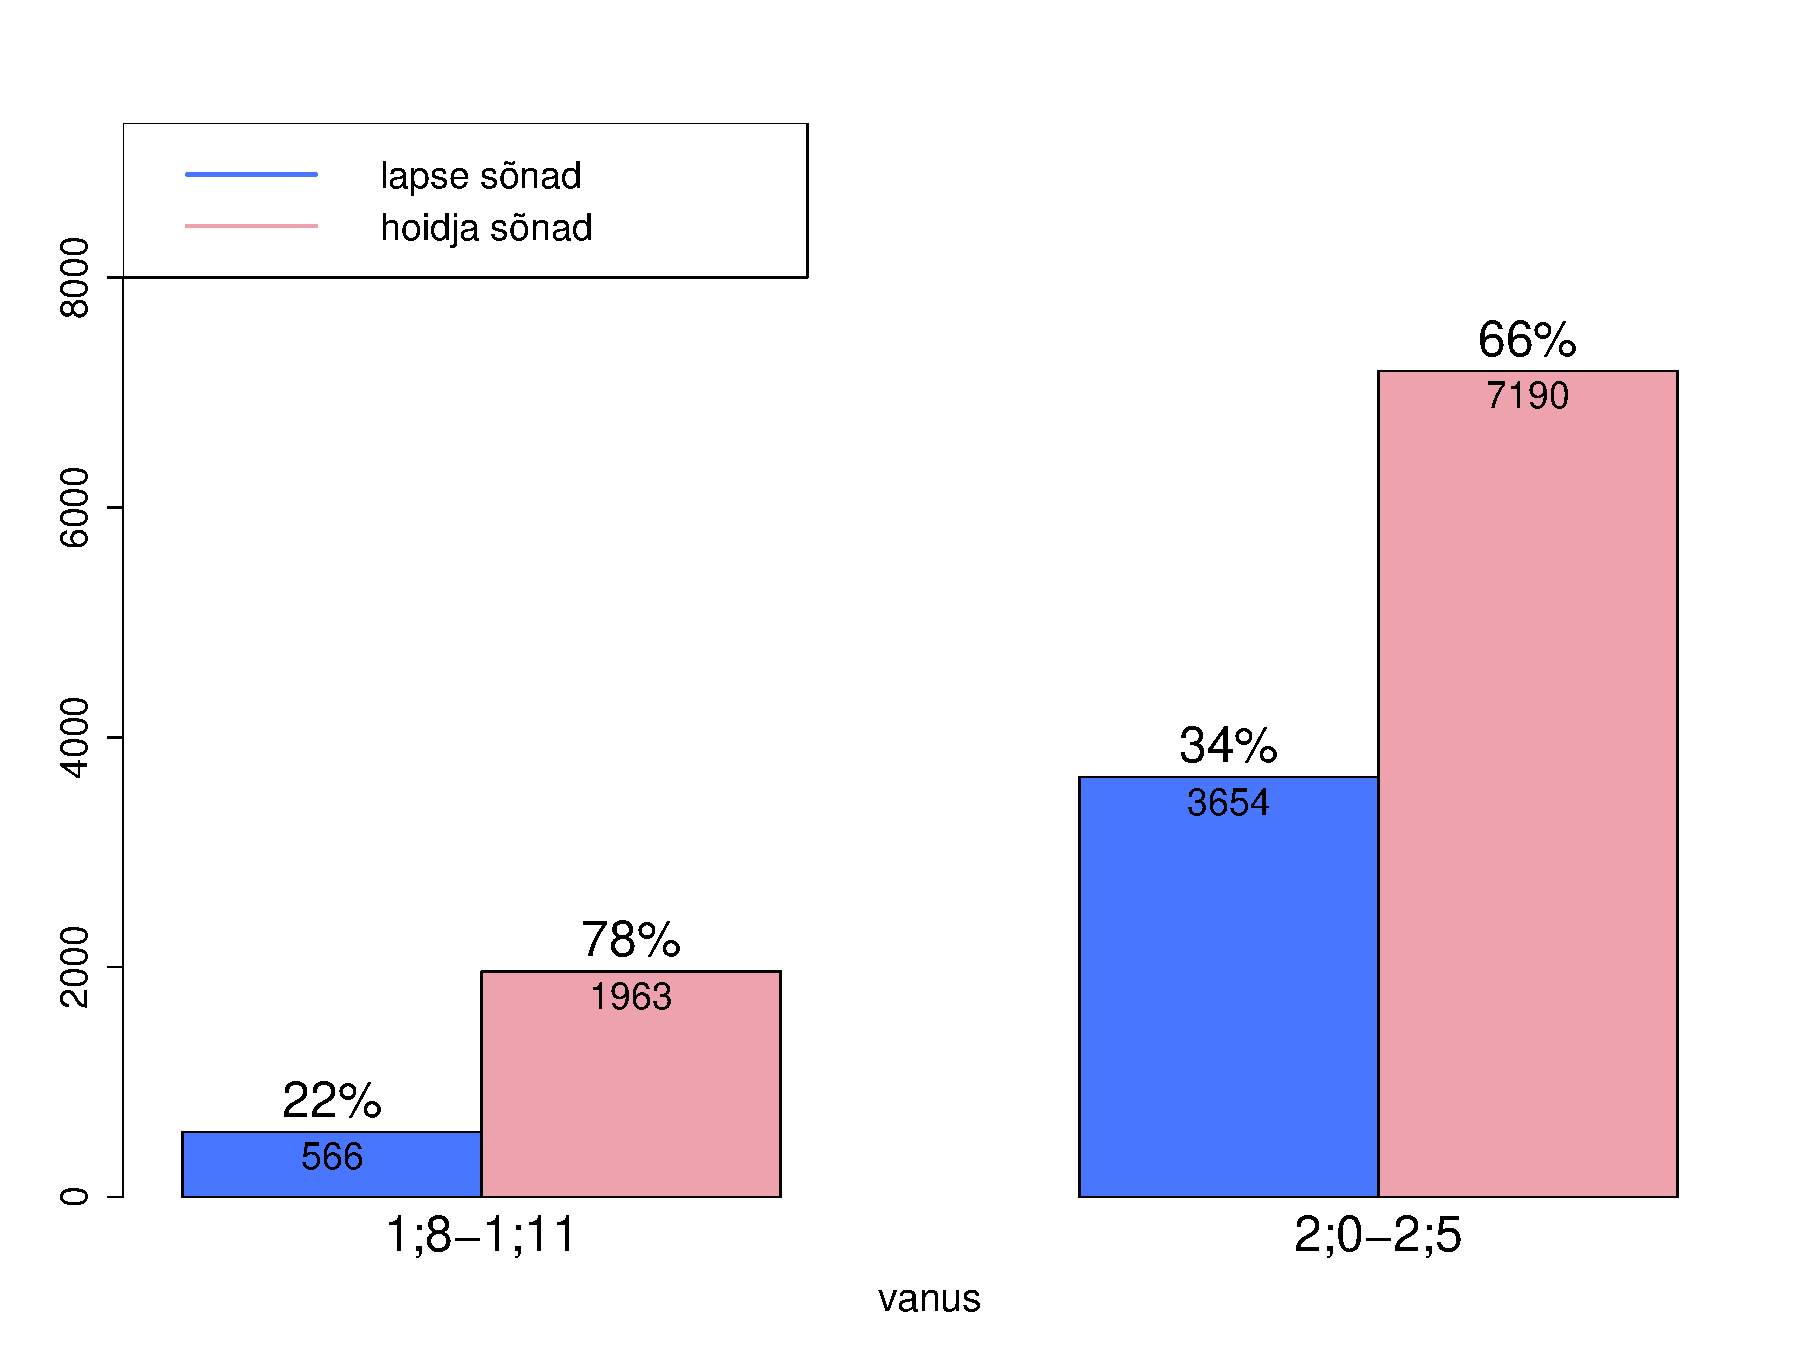
\includegraphics[width=11cm, height=9cm]{argus_vanus_sonad}
    \caption{Argus: lapse ja hoidja sõnade vanuseline jaotumine}
\end{figure}

% \begin{figure}[H]
%     \centering
%     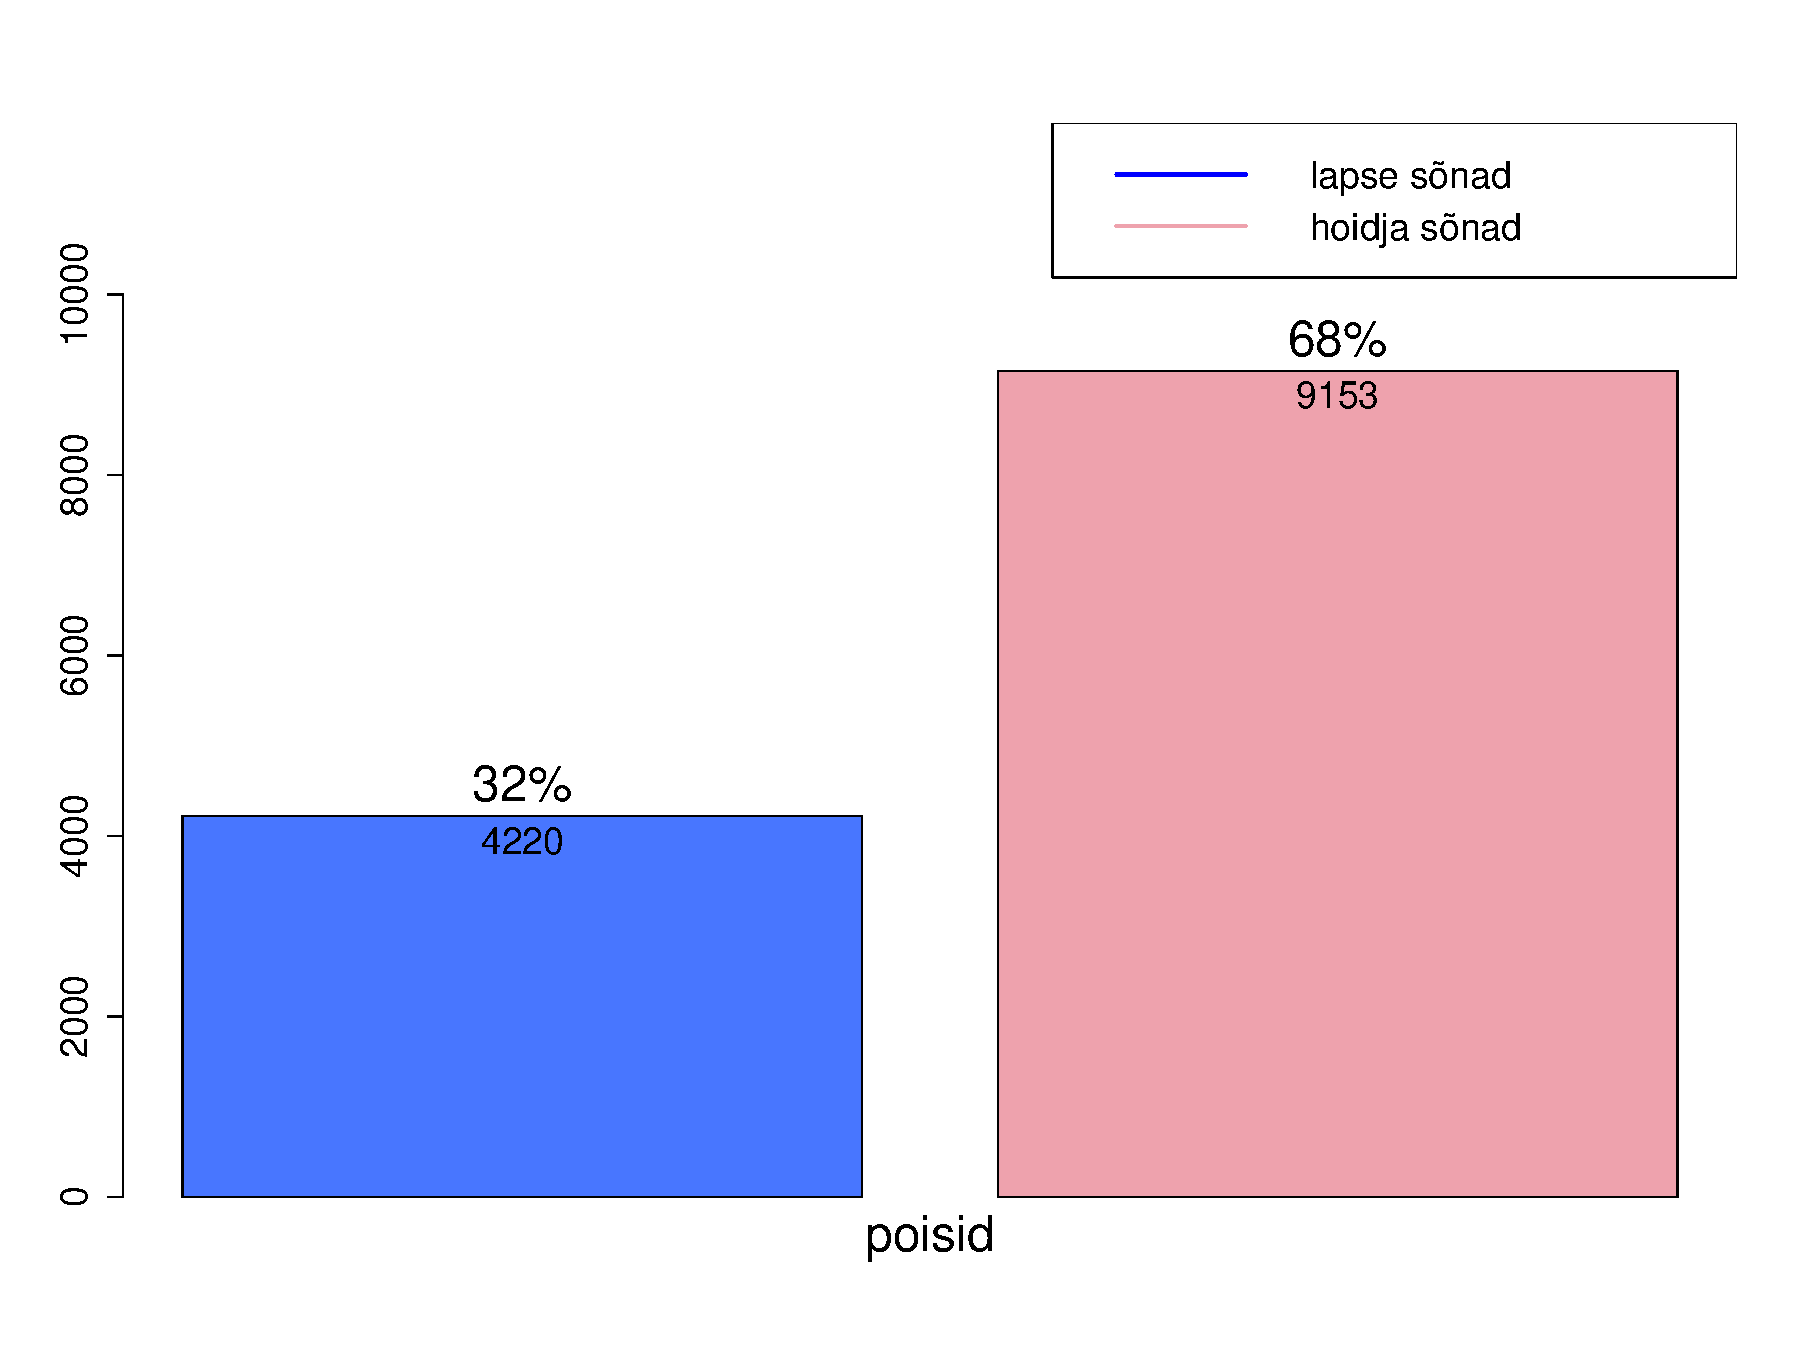
\includegraphics[width=11cm, height=9cm]{argus_sugu_sonad}
%     \caption{Argus: lapse ja hoidja sõnade sooline jaotumine}
% \end{figure}

\begin{figure}[H]
    \centering
    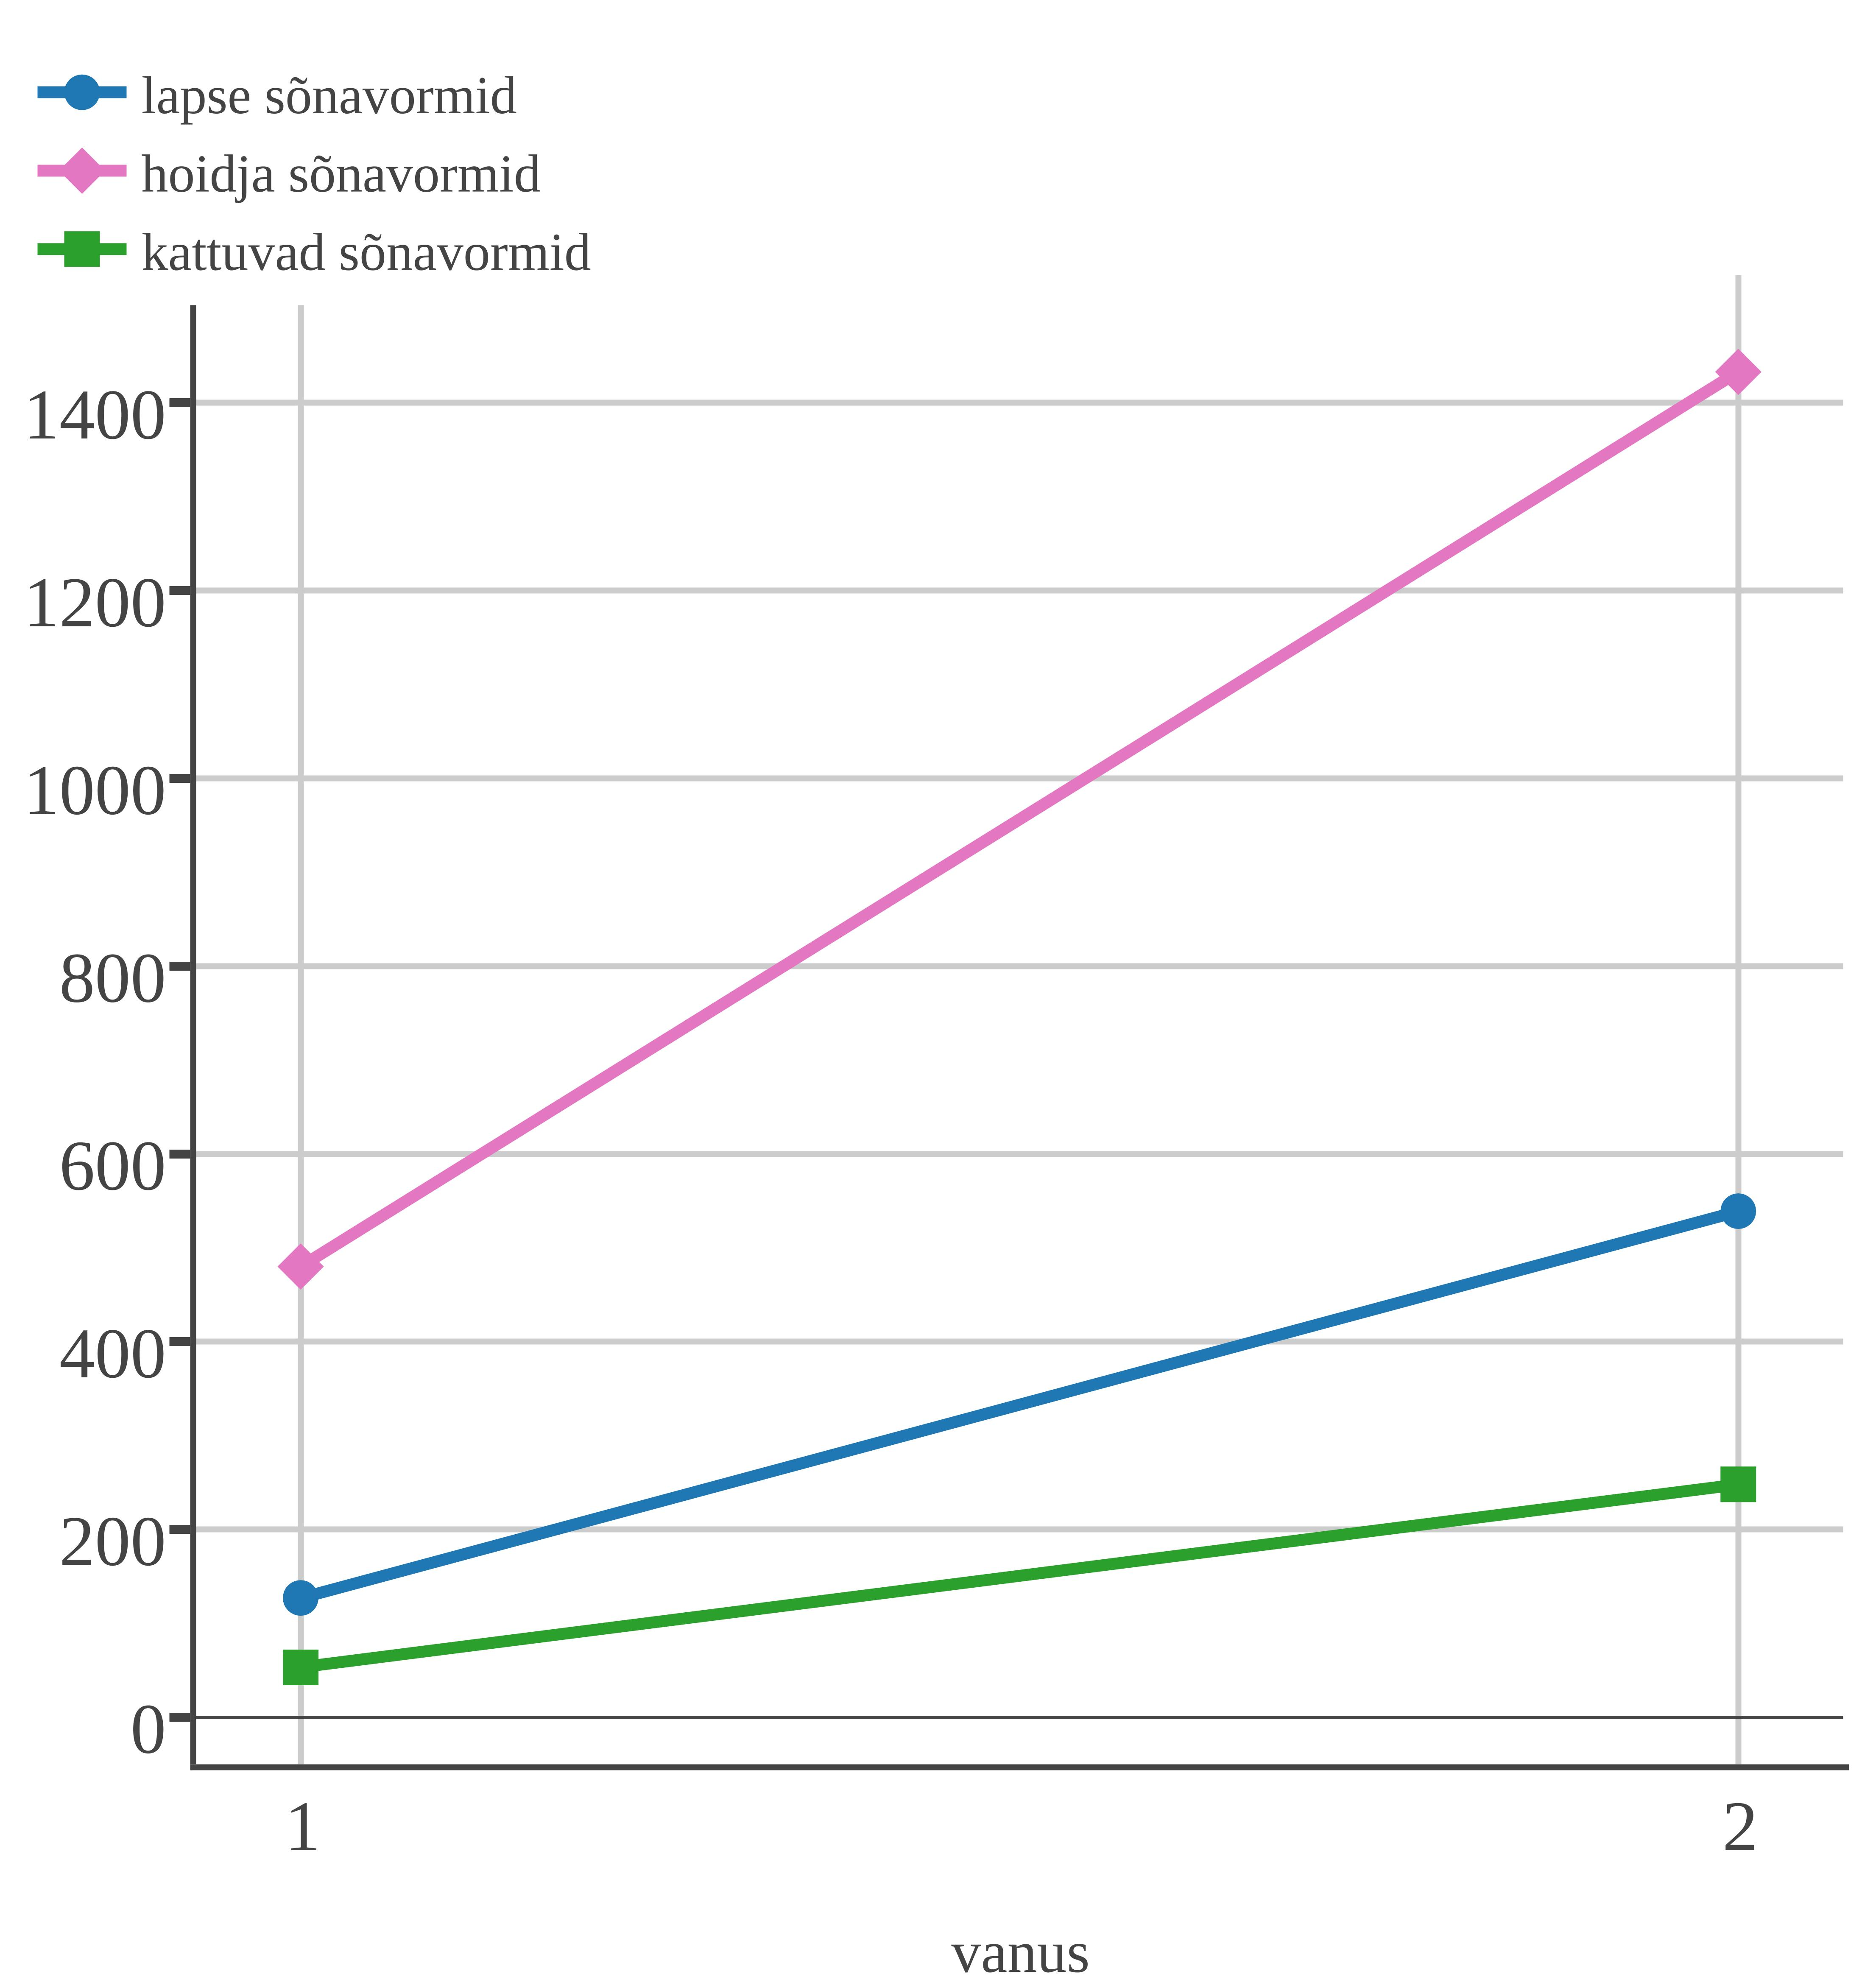
\includegraphics[width=11cm, height=9cm]{argus_kum_crop}
    \caption{Argus: sõnavormide kasv vanuseliselt}
\end{figure}



\subsubsection{Zupping}

Joonisel 18 on kujutatud lapse ja hoidja sõnade vanuselist jaotumist. Kõigis vanusegruppides on hoidja keele sõnad ülekaalus. 1-aastaste laste seas on hoidja sõnade osakaal 81\% ja lapse sõnad 19\%. 2- ja 3-aastaste laste seas on hoidja ja lapse sõnade jaotumine ühetaoline (66\% ja 34\%). 4-aastaste laste seas on hoidja sõnade osakaal 70\% ja lapse sõnu 30\%.

\begin{figure}[H]
    \centering
    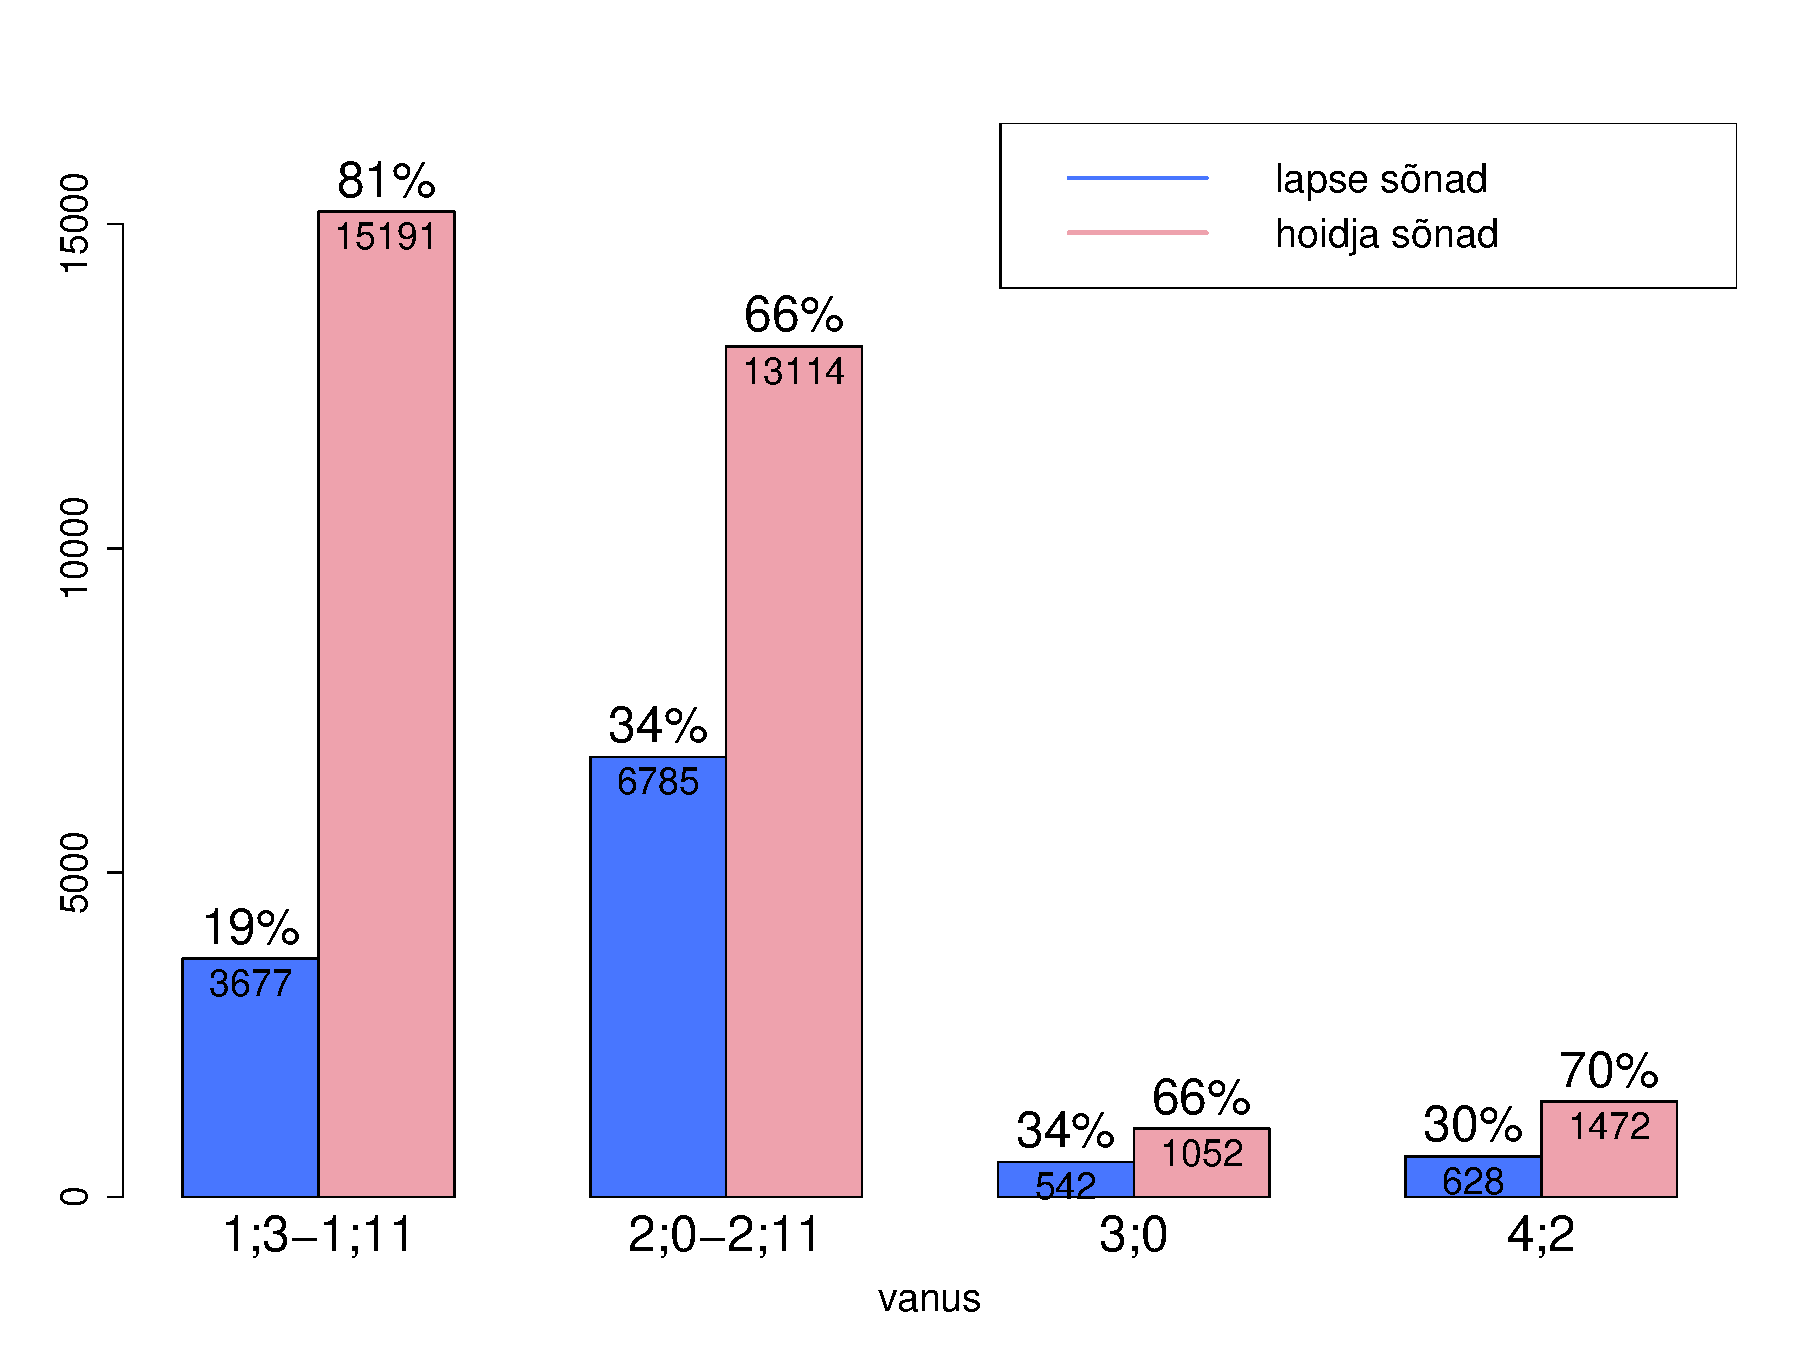
\includegraphics[width=11cm, height=9cm]{zupping_vanus_sonad}
    \caption{Zupping: lapse ja hoidja sõnade vanuseline jaotumine}
\end{figure}

% \begin{figure}[H]
%     \centering
%     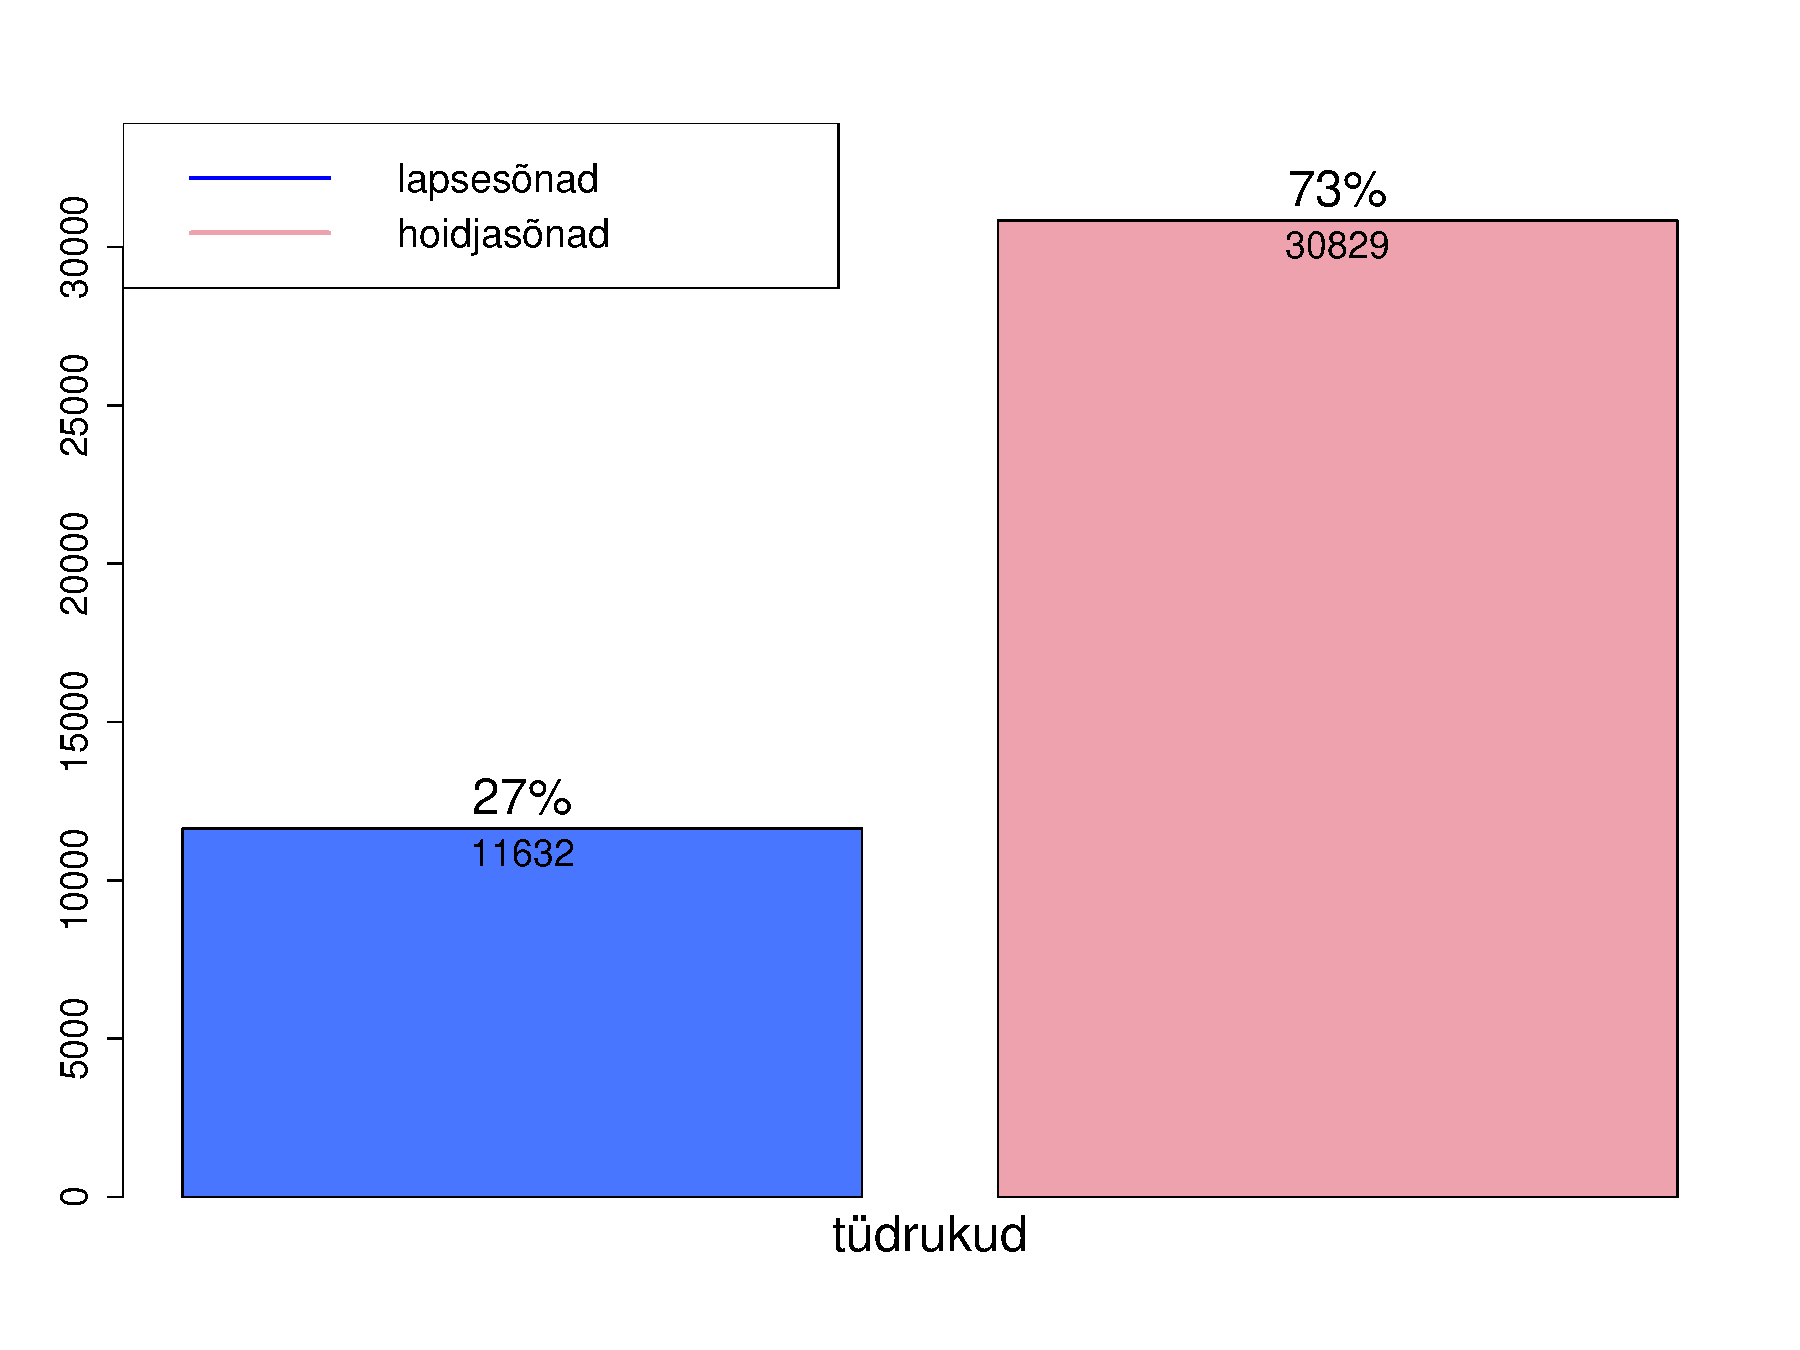
\includegraphics[width=11cm, height=9cm]{zupping_sugu_sonad}
%     \caption{Zupping: lapse ja hoidja sõnade sooline jaotumine}
% \end{figure}

\begin{figure}[H]
    \centering
    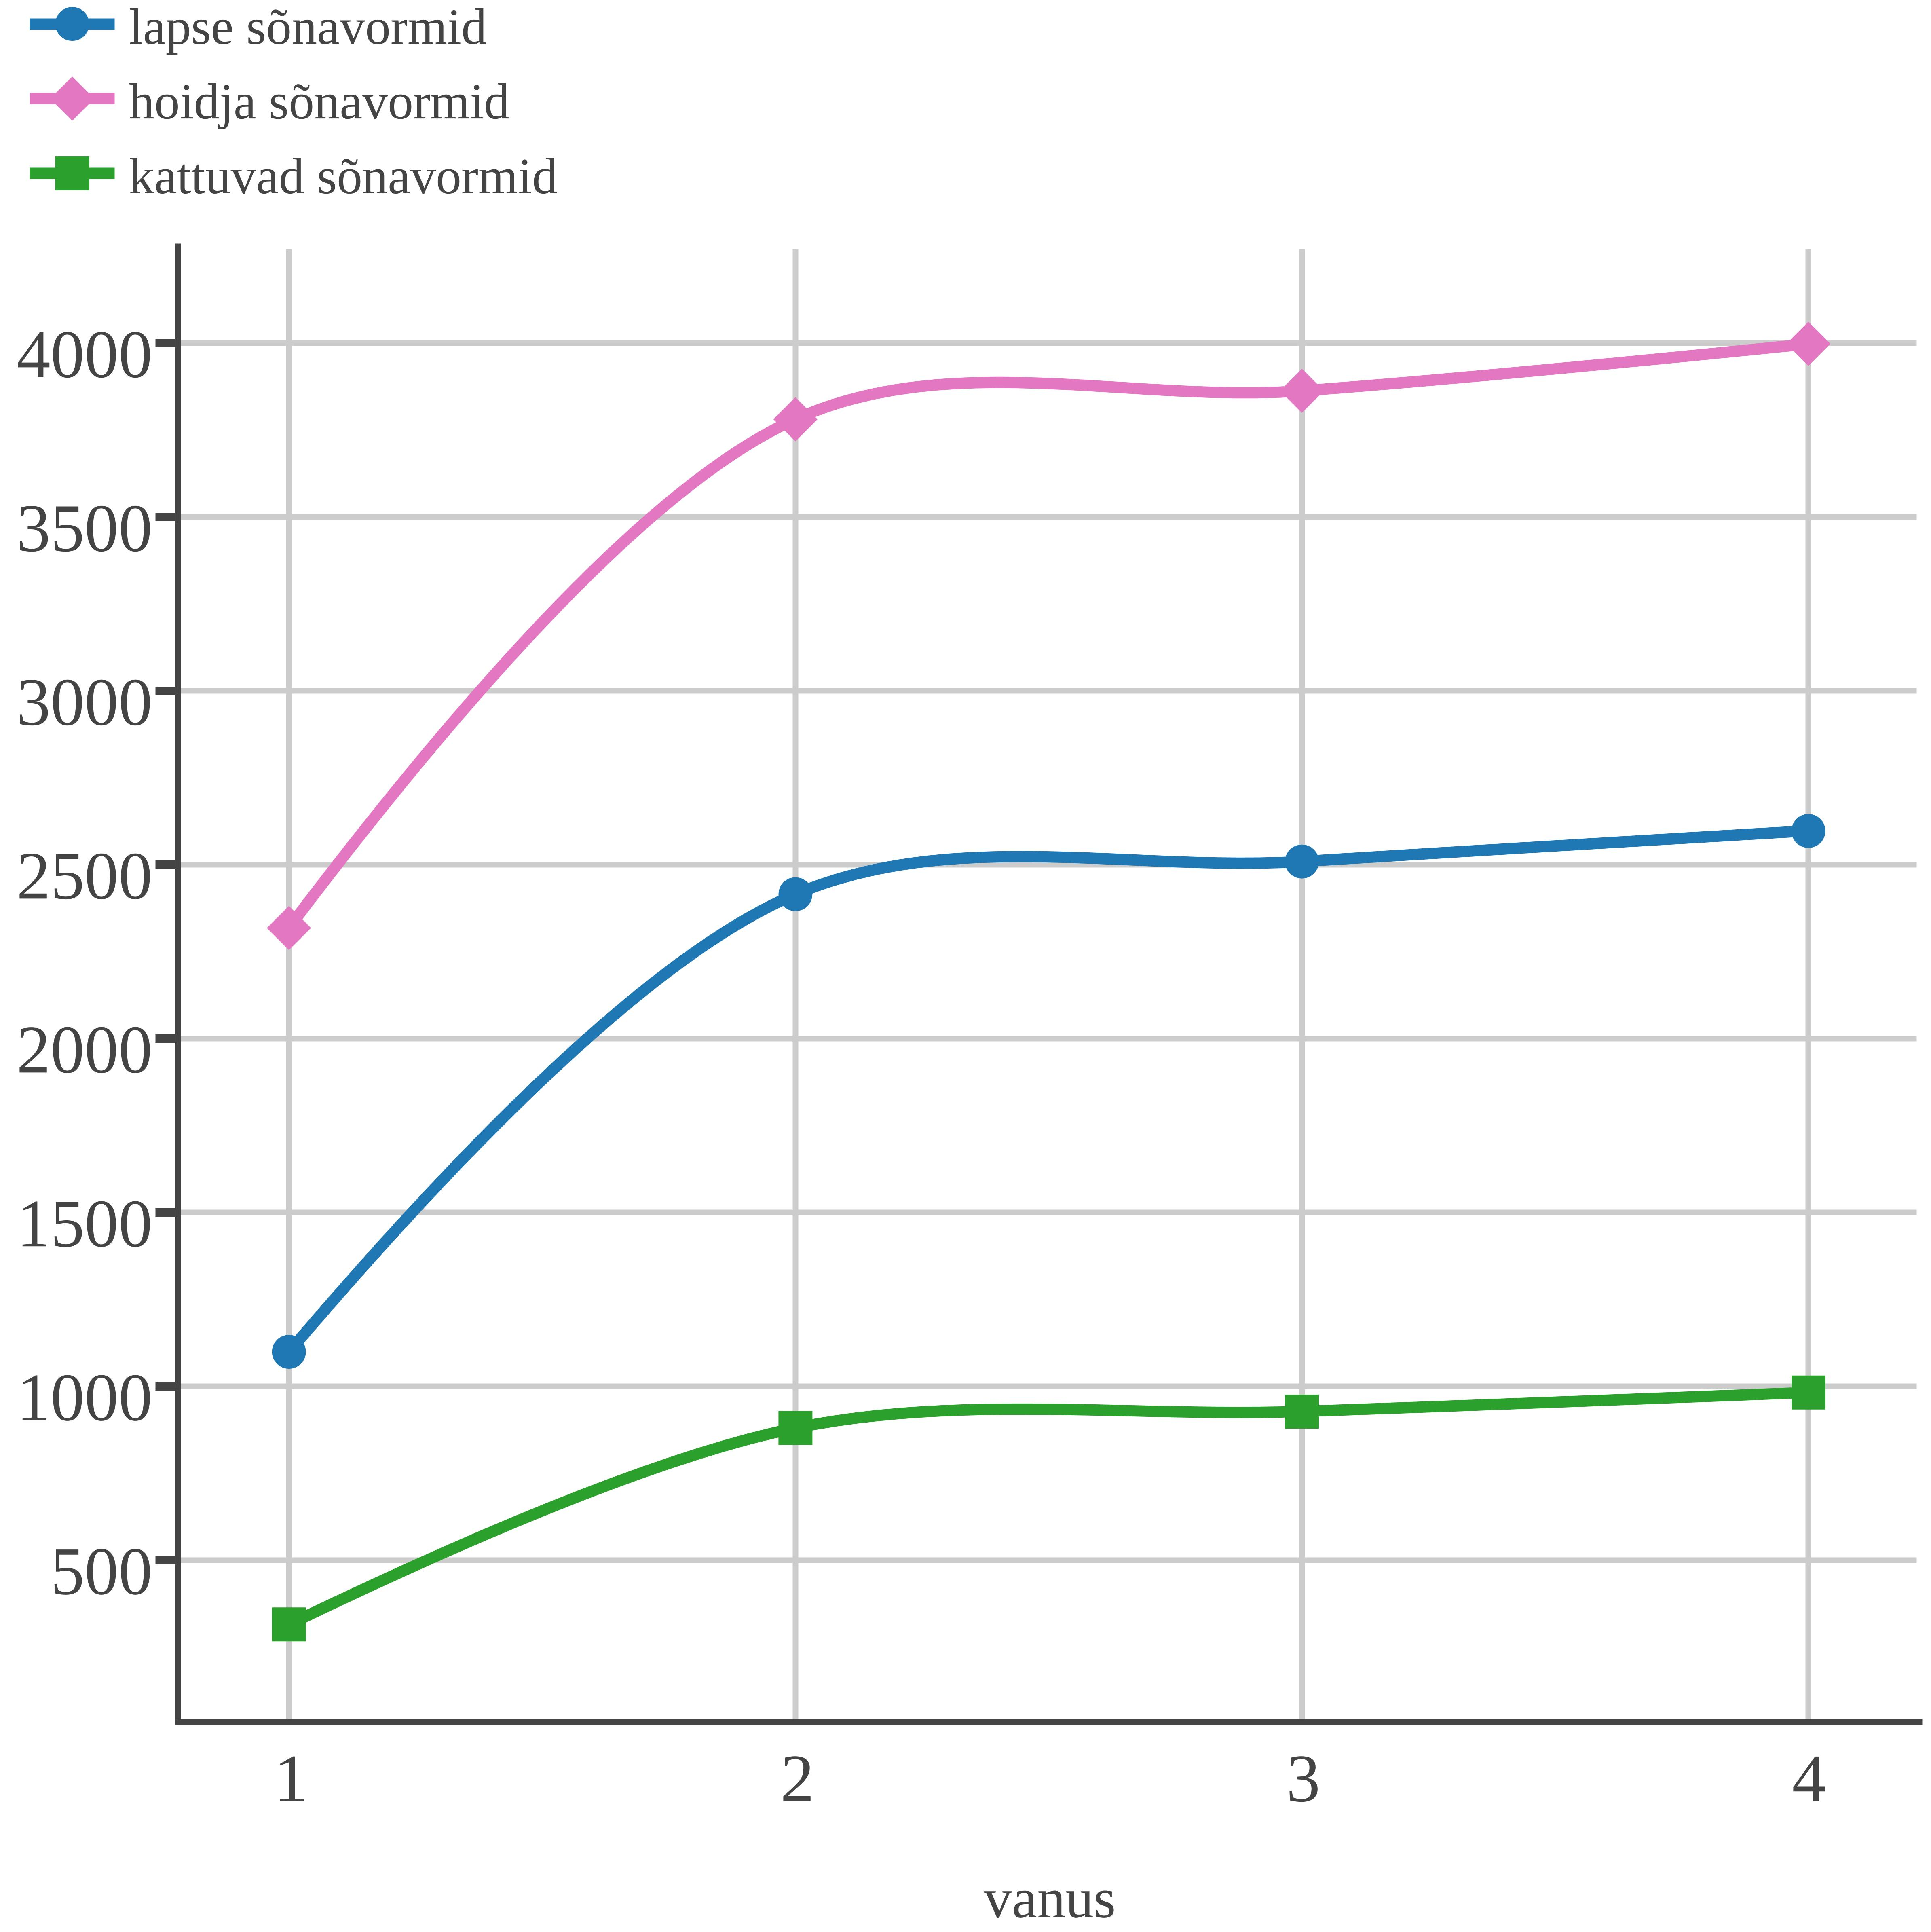
\includegraphics[width=11cm, height=9cm]{zupping_kum_crop}
    \caption{Zupping: sõnavormide kasv vanuseliselt}
\end{figure}



\subsubsection{Kõik alamkorpused}



\begin{figure}[H]
    \centering
    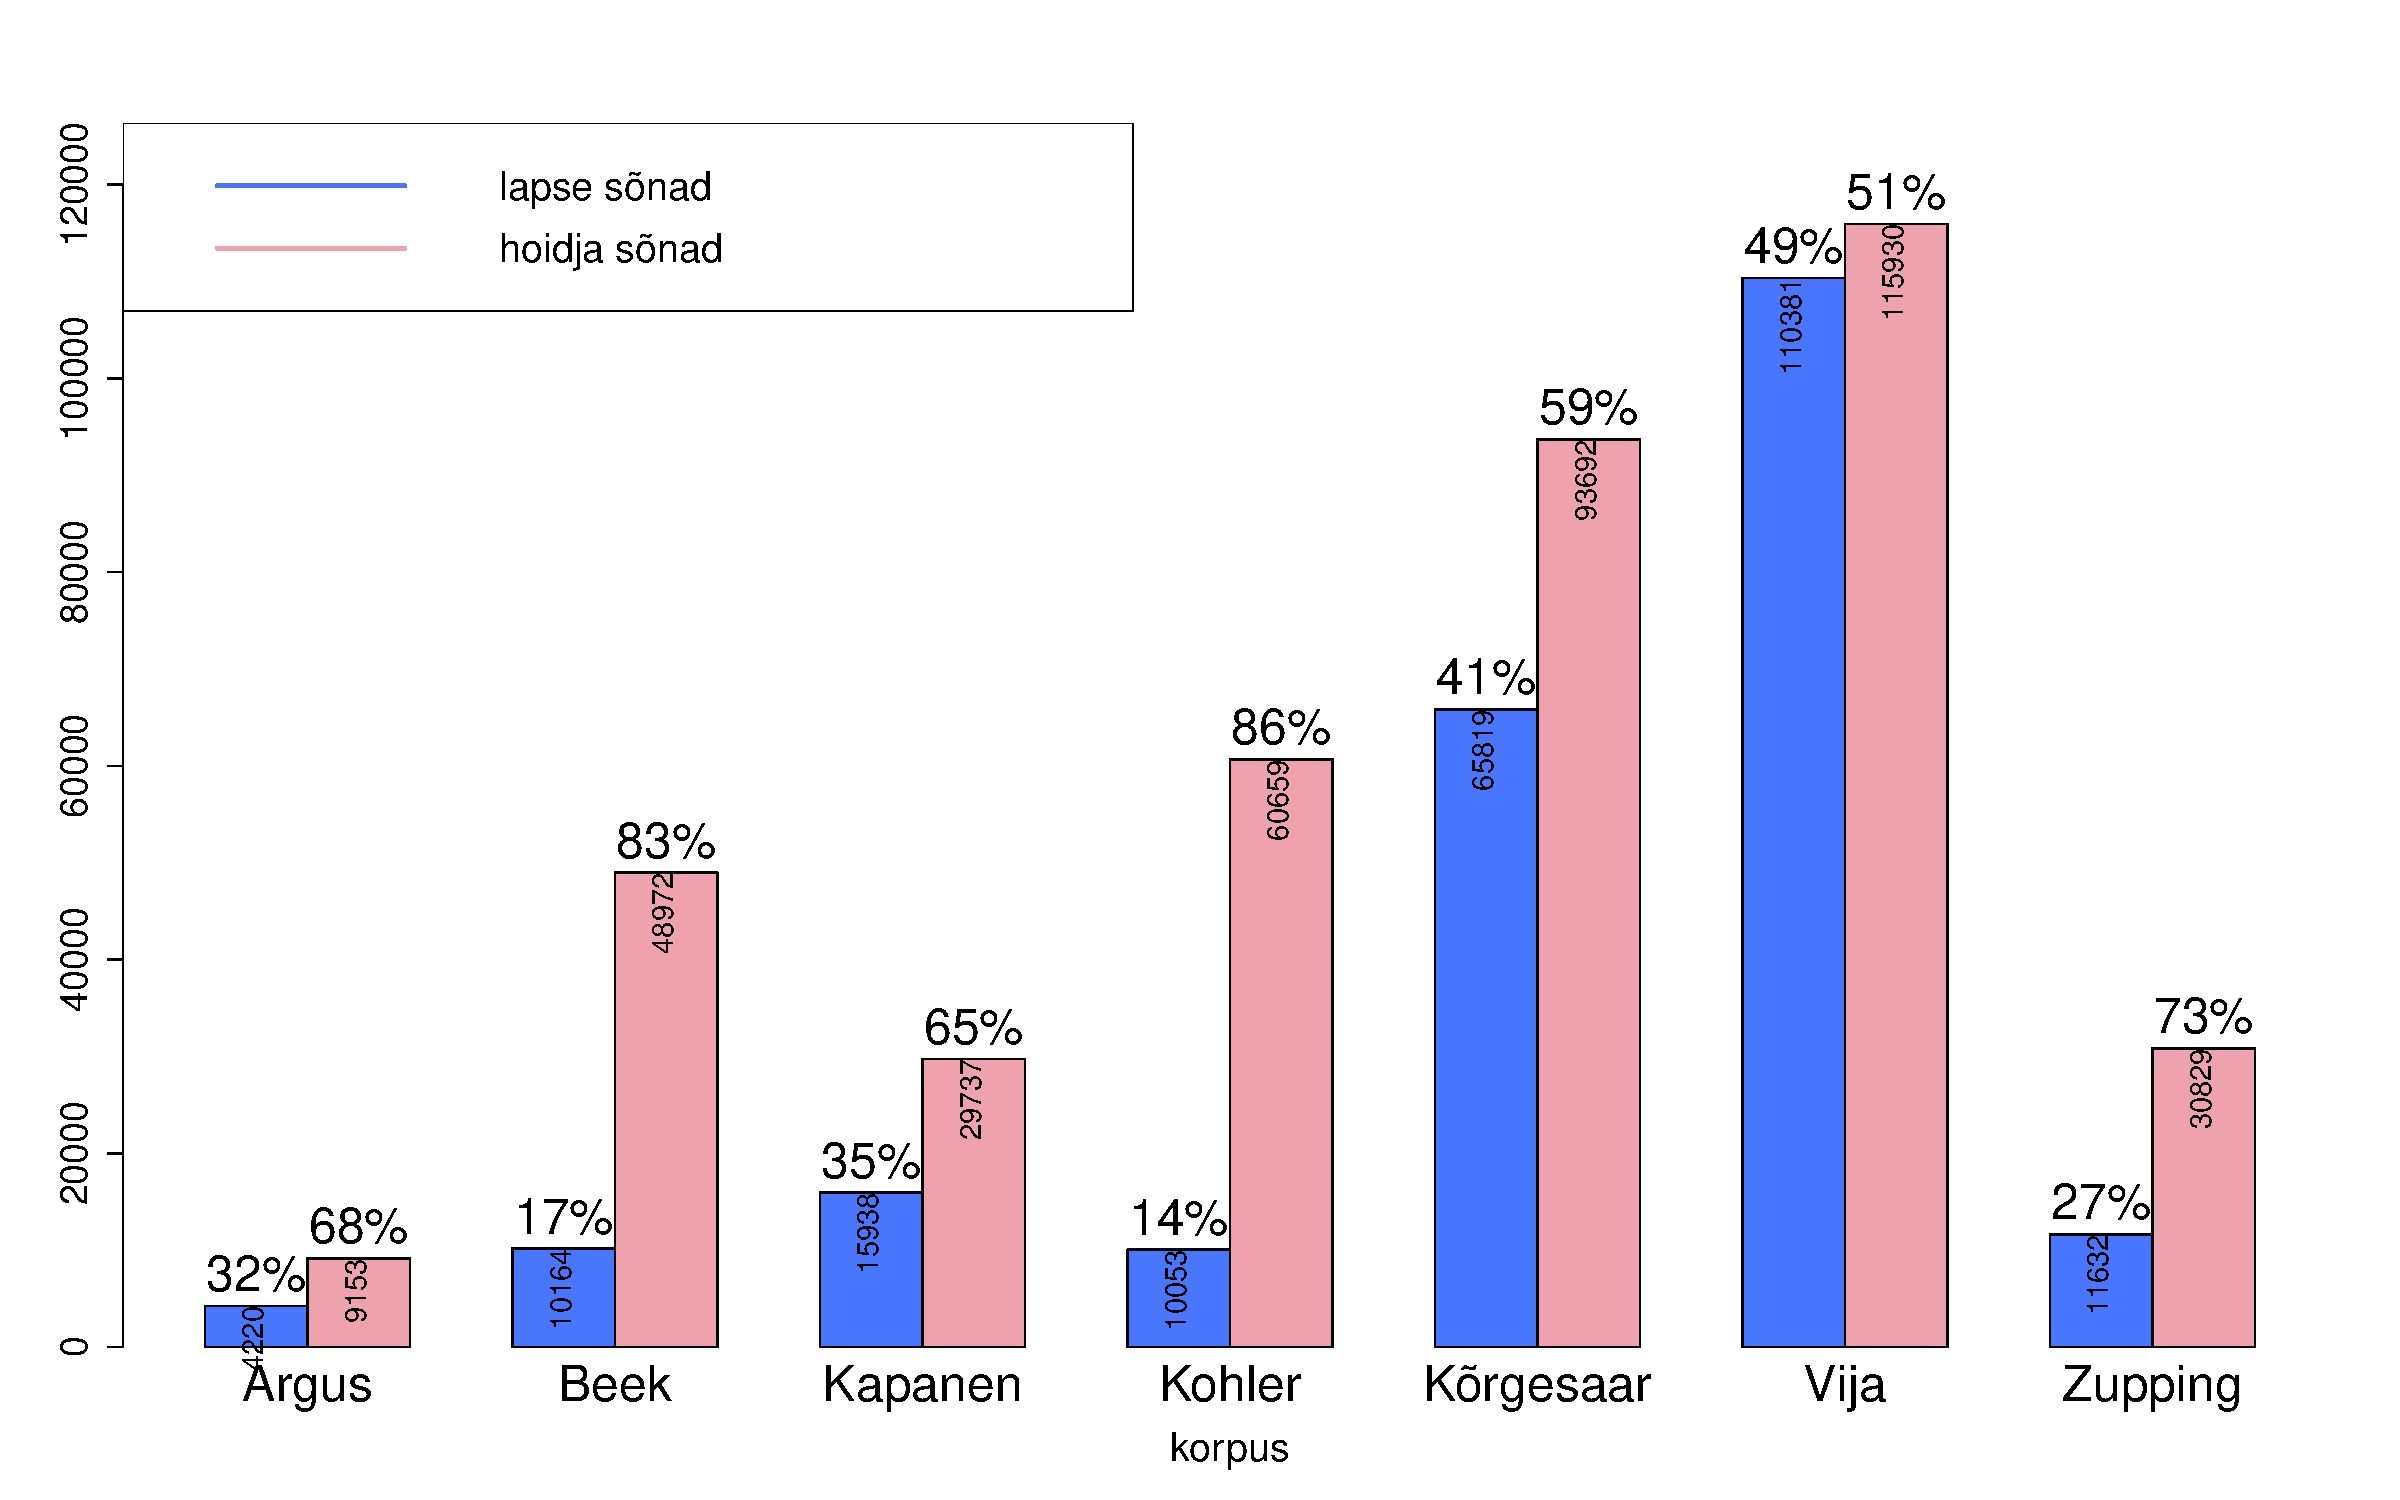
\includegraphics[width=\textwidth]{koik_korpus_sonad}
    \caption{hoidja ja lapse sõnade jaotumine korpustes}
\end{figure}


\begin{table}[H]
\centering
\caption{Sõnavormide jaotumine alamkorpustes}
\begin{tabular}{|l|c|c|c|c|}
\hline
korpus    & \multicolumn{1}{l|}{lapse sõnavormid}               & \multicolumn{1}{l|}{hoidja sõnavormid}              & \multicolumn{1}{l|}{kattuvad sõnavormid}            & \multicolumn{1}{l|}{KOKKU}                            \\ \hline\hline
Argus     & \begin{tabular}[c]{@{}c@{}}291\\ 17\%\end{tabular}  & \begin{tabular}[c]{@{}c@{}}1185\\ 69\%\end{tabular} & \begin{tabular}[c]{@{}c@{}}248\\ 14\%\end{tabular}  & \begin{tabular}[c]{@{}c@{}}1724\\ 100\%\end{tabular}  \\ \hline
Beek      & \begin{tabular}[c]{@{}c@{}}732\\ 16\%\end{tabular}  & \begin{tabular}[c]{@{}c@{}}3517\\ 78\%\end{tabular} & \begin{tabular}[c]{@{}c@{}}272\\ 6\%\end{tabular}   & \begin{tabular}[c]{@{}c@{}}4521\\ 100\%\end{tabular}  \\ \hline
Kapanen   & \begin{tabular}[c]{@{}c@{}}2661\\ 39\%\end{tabular} & \begin{tabular}[c]{@{}c@{}}2708\\ 39\%\end{tabular} & \begin{tabular}[c]{@{}c@{}}1533\\ 22\%\end{tabular} & \begin{tabular}[c]{@{}c@{}}6902\\ 100\%\end{tabular}  \\ \hline
Kohler    & \begin{tabular}[c]{@{}c@{}}817\\ 17\%\end{tabular}  & \begin{tabular}[c]{@{}c@{}}2700\\ 58\%\end{tabular} & \begin{tabular}[c]{@{}c@{}}1160\\ 25\%\end{tabular} & \begin{tabular}[c]{@{}c@{}}4677\\ 100\%\end{tabular}  \\ \hline
Kõrgesaar & \begin{tabular}[c]{@{}c@{}}5402\\ 35\%\end{tabular} & \begin{tabular}[c]{@{}c@{}}5665\\ 36\%\end{tabular} & \begin{tabular}[c]{@{}c@{}}4455\\ 29\%\end{tabular} & \begin{tabular}[c]{@{}c@{}}15522\\ 100\%\end{tabular} \\ \hline
Vija      & \begin{tabular}[c]{@{}c@{}}4834\\ 35\%\end{tabular} & \begin{tabular}[c]{@{}c@{}}4484\\ 32\%\end{tabular} & \begin{tabular}[c]{@{}c@{}}4643\\ 33\%\end{tabular} & \begin{tabular}[c]{@{}c@{}}13961\\ 100\%\end{tabular} \\ \hline
Zupping   & \begin{tabular}[c]{@{}c@{}}1615\\ 29\%\end{tabular} & \begin{tabular}[c]{@{}c@{}}3016\\ 54\%\end{tabular} & \begin{tabular}[c]{@{}c@{}}982\\ 17\%\end{tabular}  & \begin{tabular}[c]{@{}c@{}}5613\\ 100\%\end{tabular}  \\ \hline
\end{tabular}
\end{table}

% \begin{figure}[H]
%     \centering
%     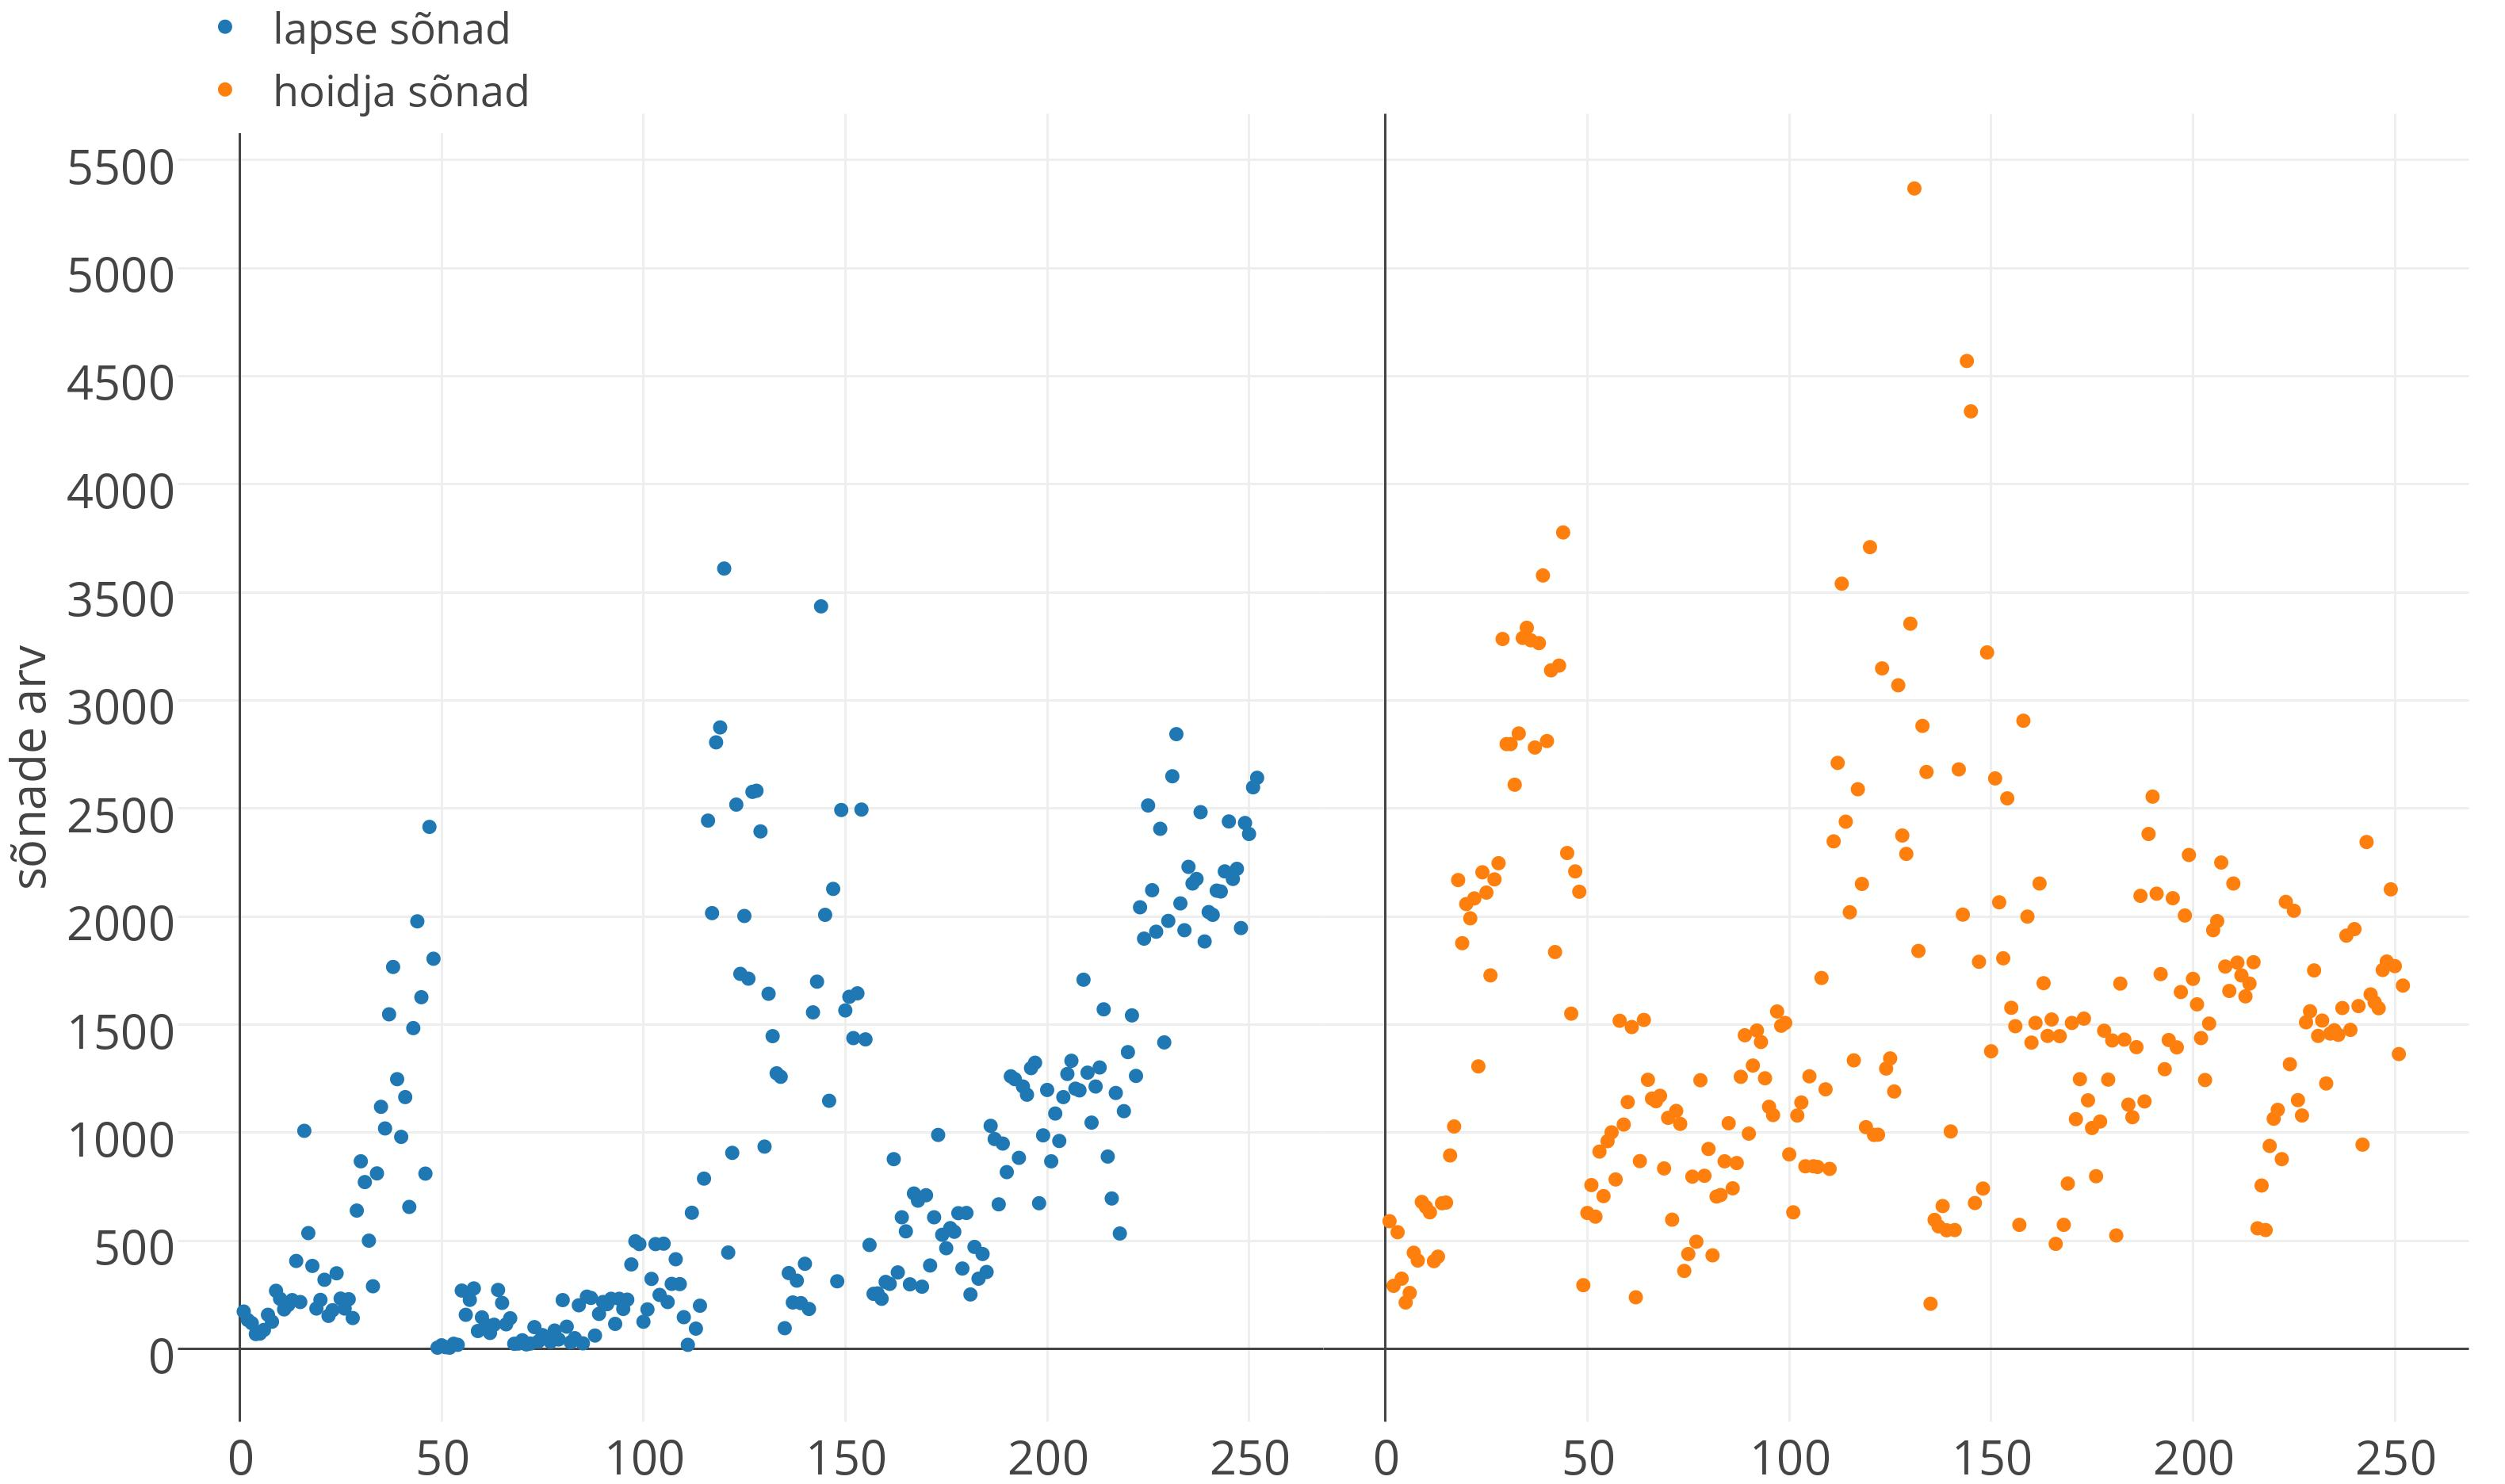
\includegraphics[width=\textwidth, height=9cm]{hoidja_lapse_sonad_crop}
%     \caption{hoidja ja lapse sõnade jaotumine kogu korpuses}
% \end{figure}

\begin{figure}[H]
    \centering
    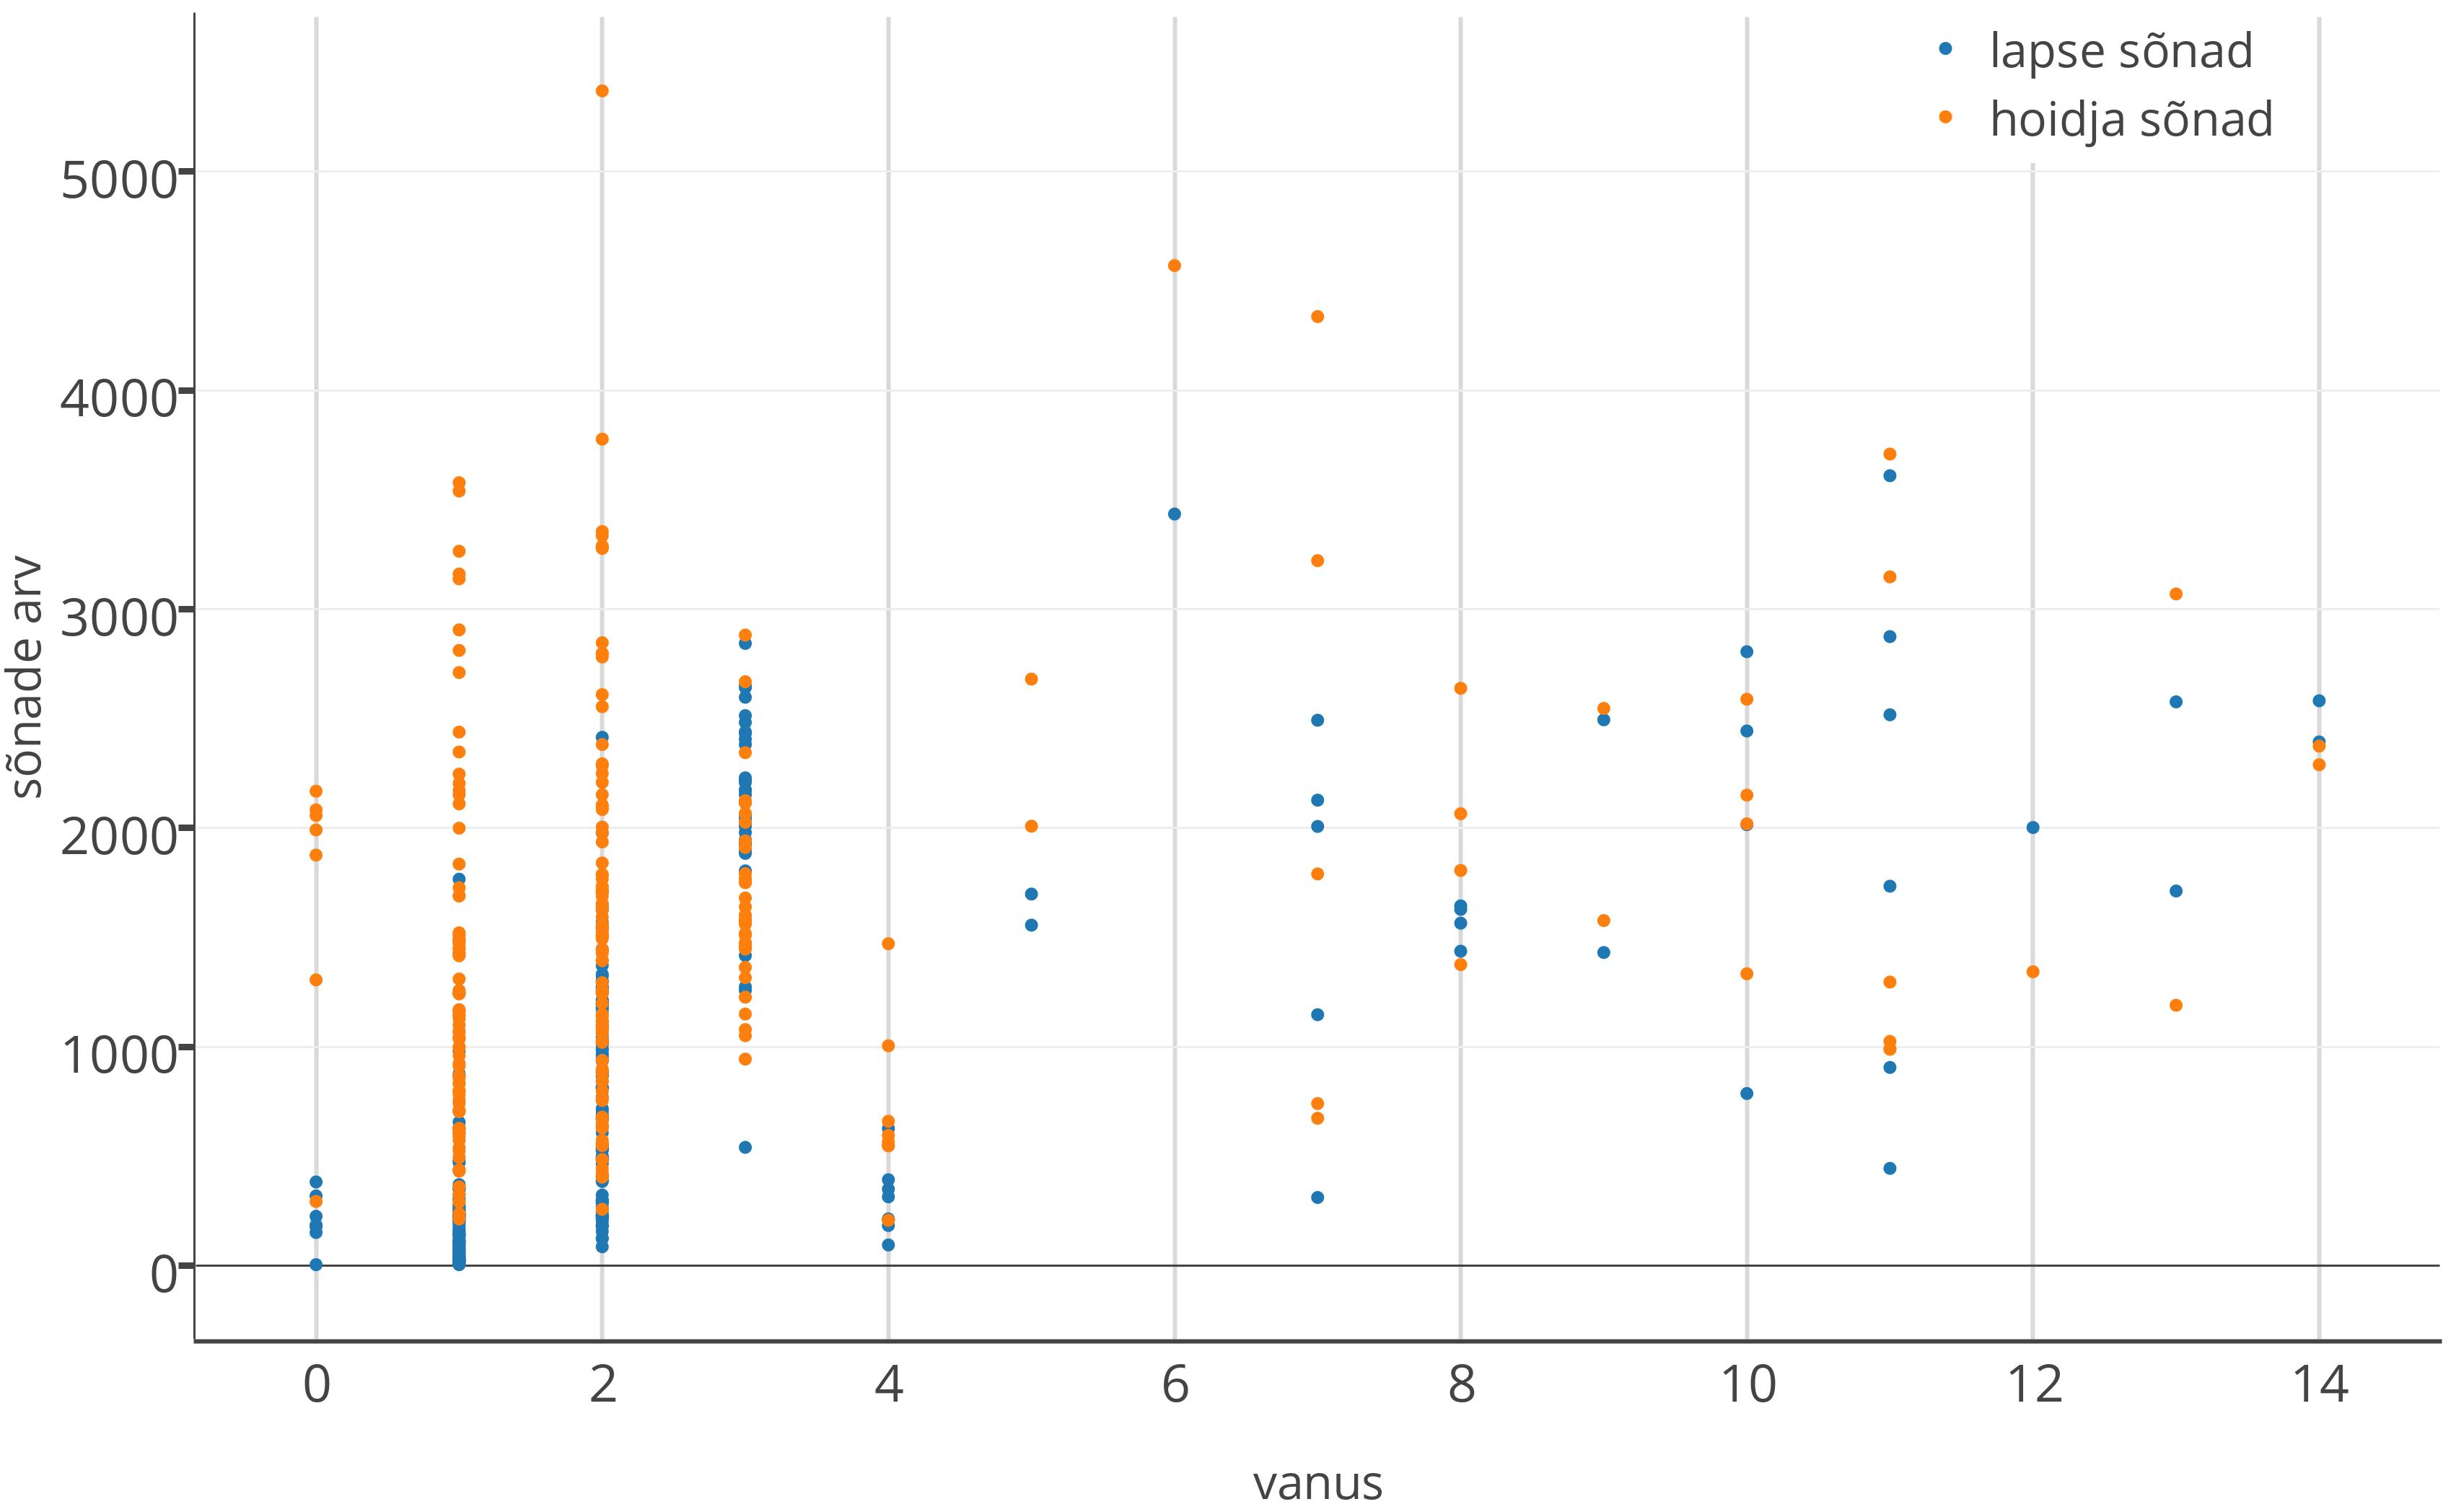
\includegraphics[width=\textwidth, height=9cm]{lindistused_vanus_sonad_crop}
    \caption{hoidja ja lapse sõnade vanuseline jaotumine kogu korpuses}
\end{figure}


\begin{figure}[H]
    \centering
    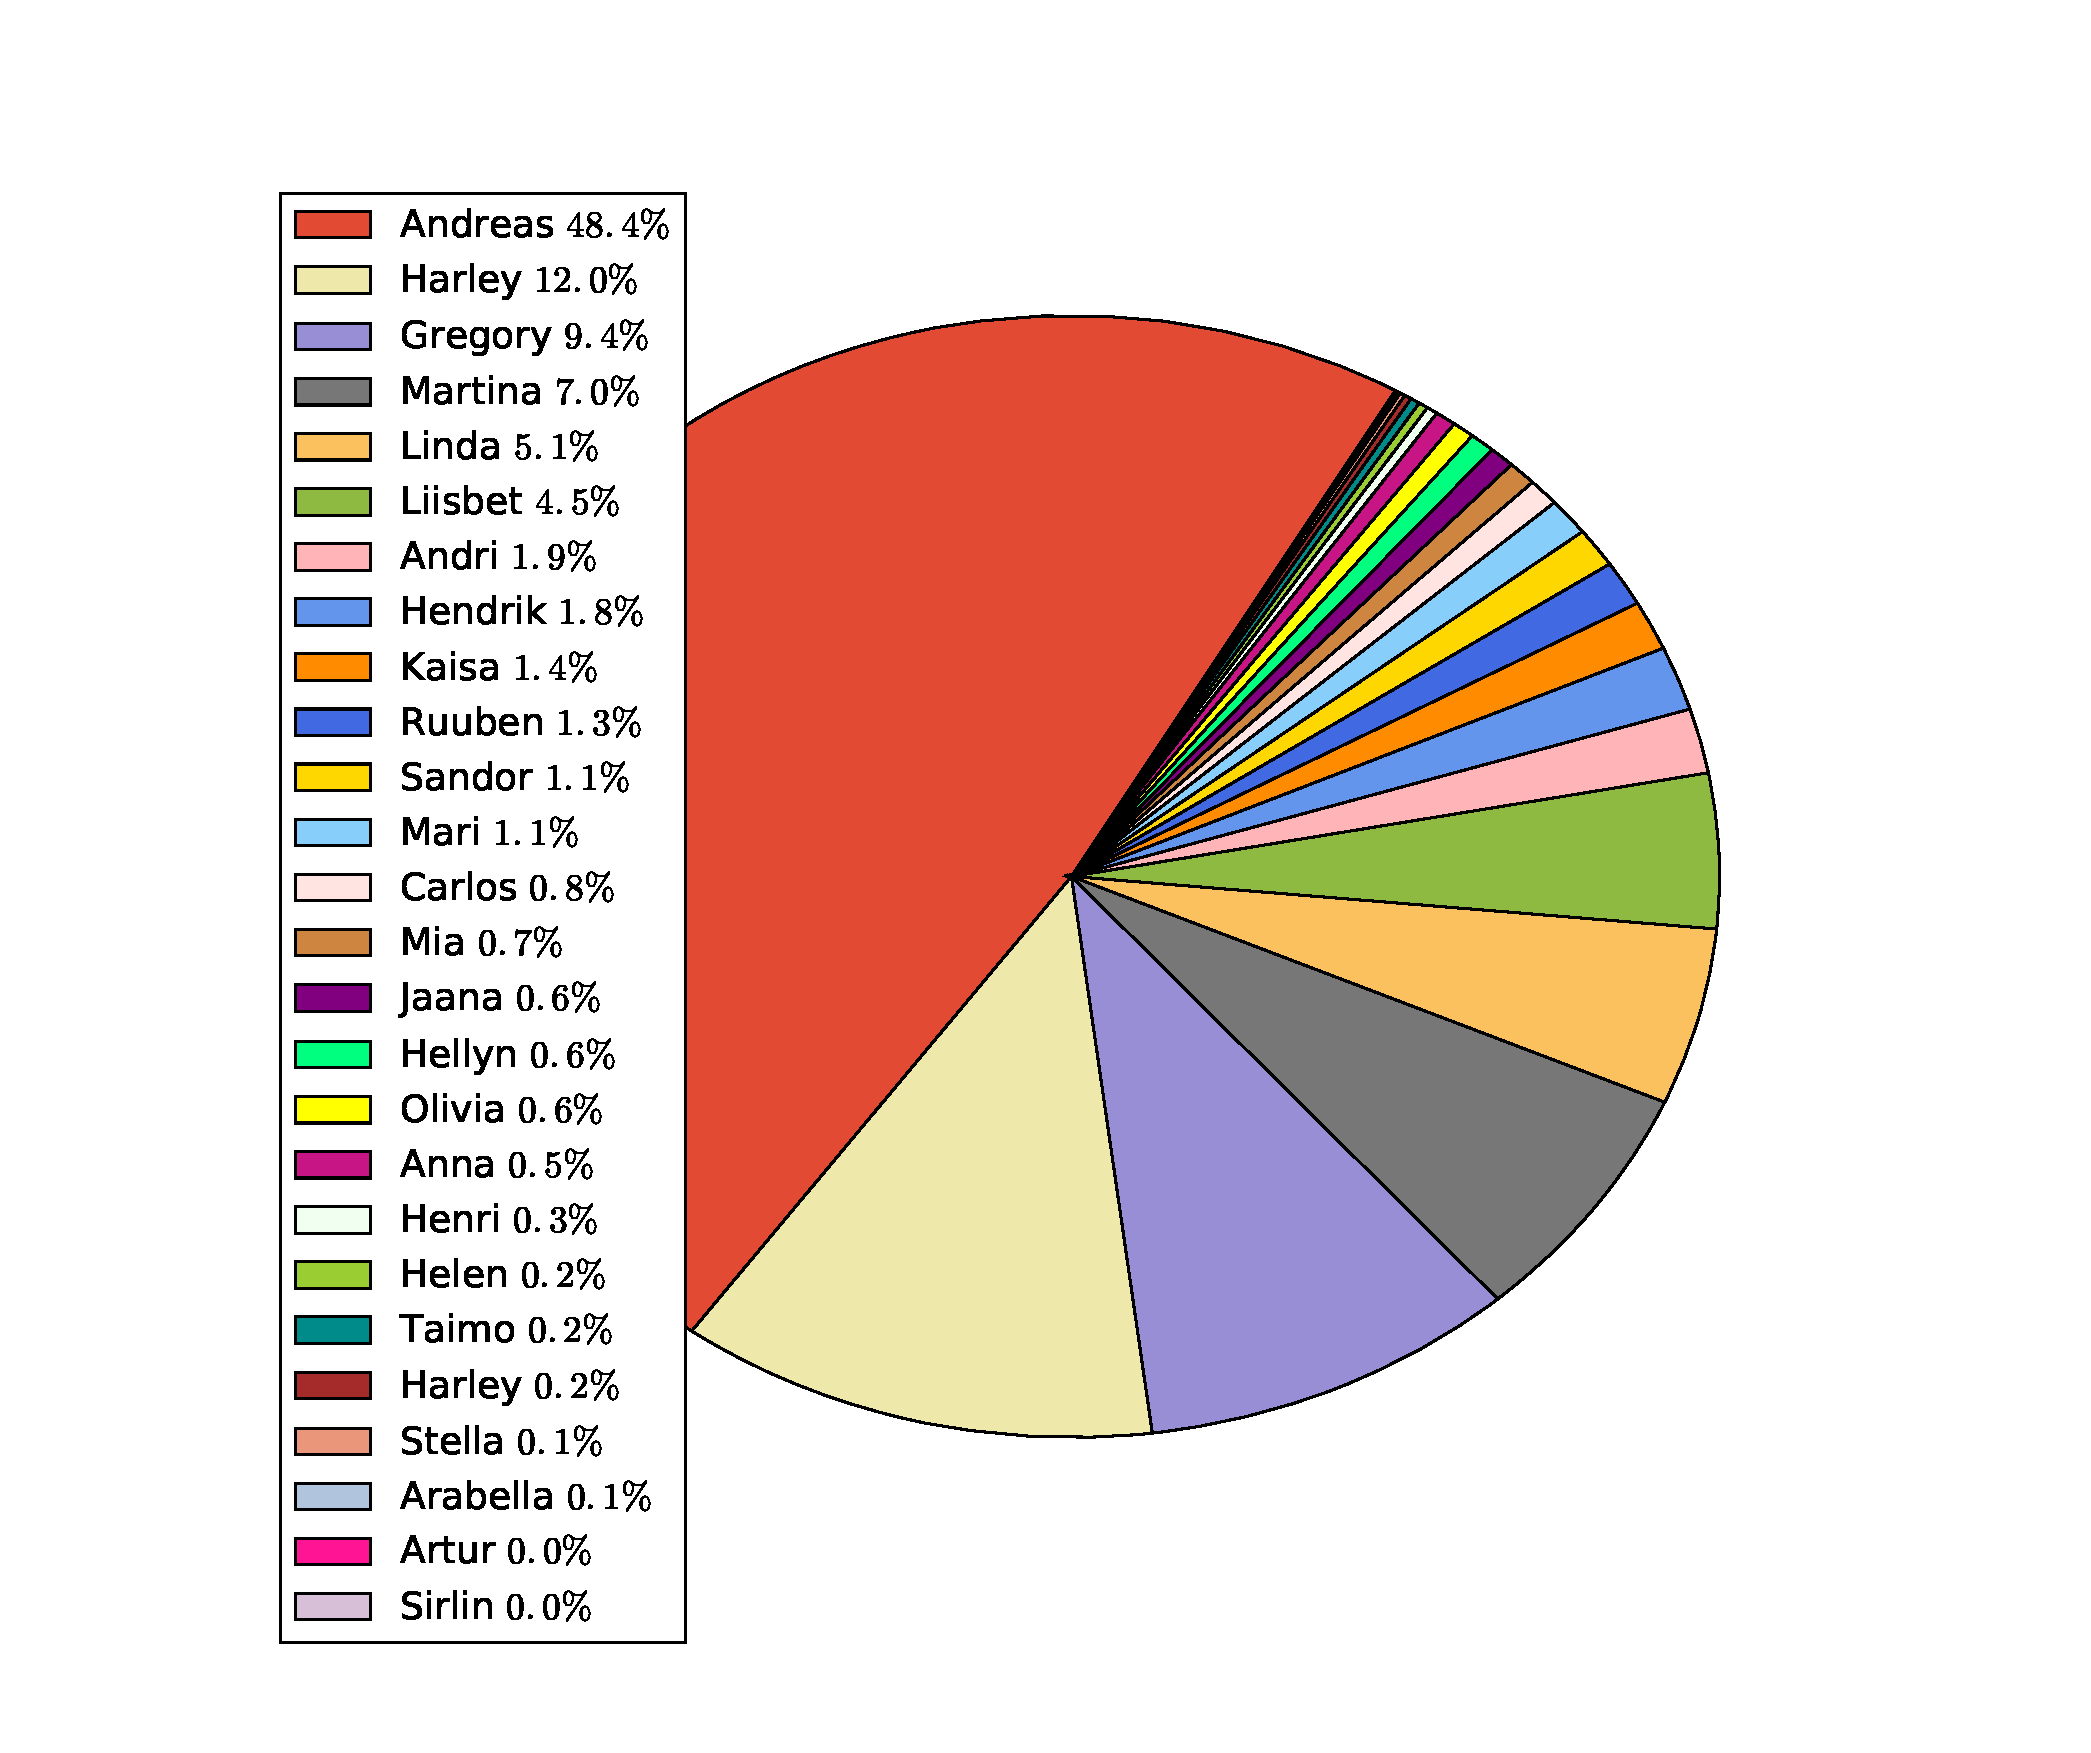
\includegraphics[width=\textwidth]{lapse_sonad_kogu_korpus}
    \caption{lapse sõnade jaotumine kogu korpuses}
\end{figure}

\begin{figure}[H]
    \centering
    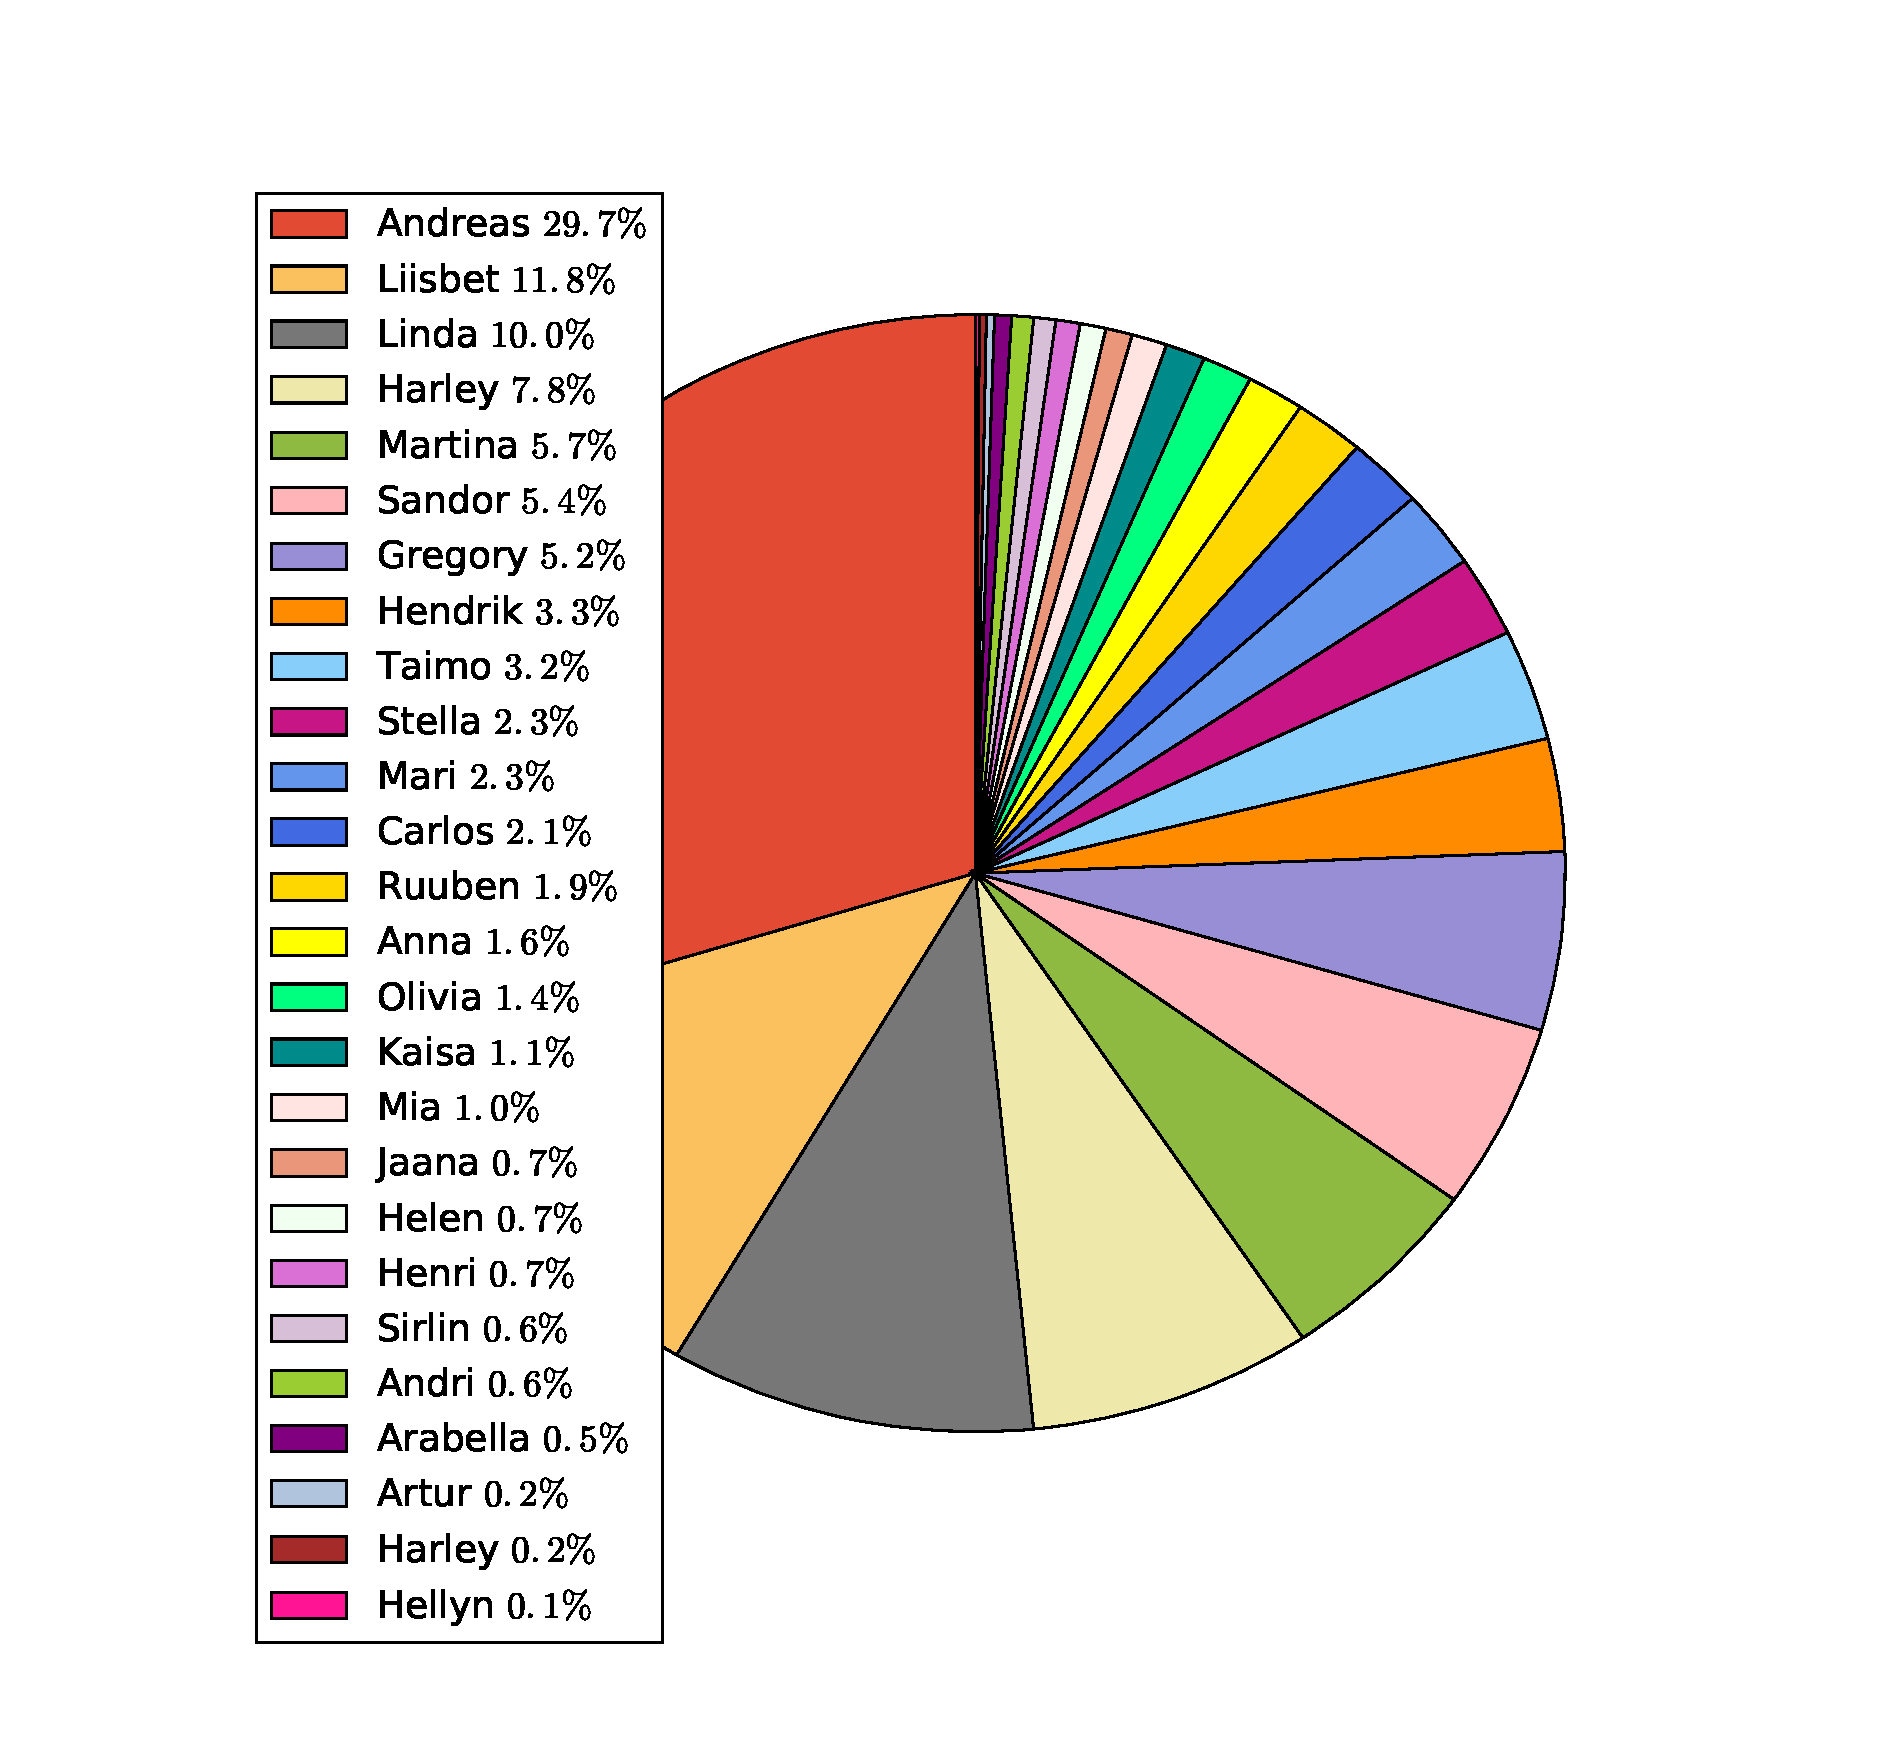
\includegraphics[width=\textwidth]{hoidja_sonad_kogu_korpuses}
    \caption{hoidja sõnade jaotumine kogu korpuses}
\end{figure}

\begin{figure}[H]
    \centering
    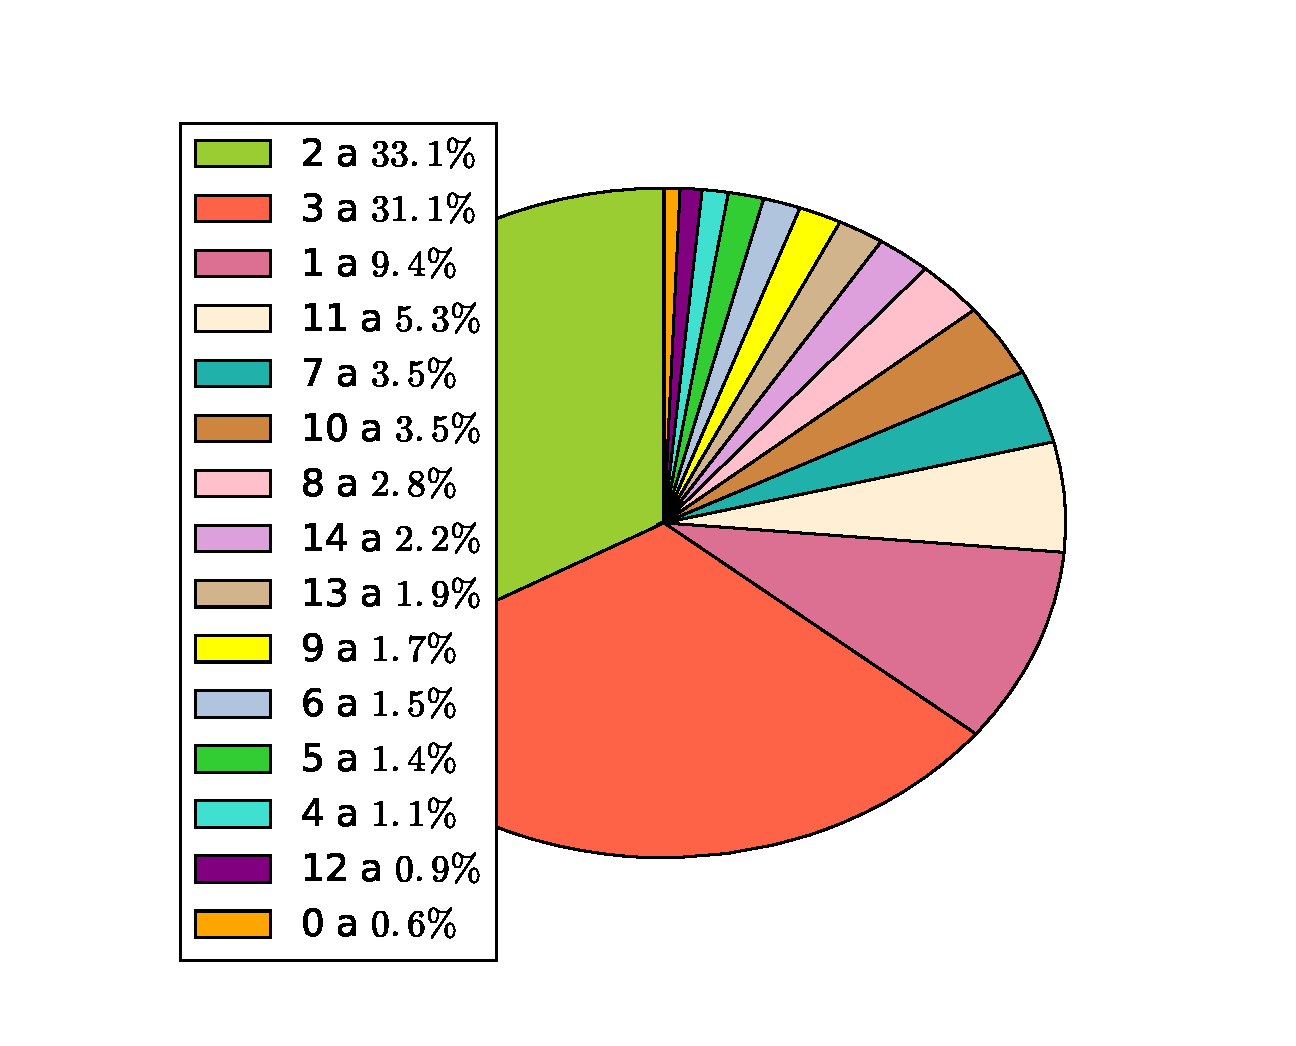
\includegraphics[width=\textwidth]{vanus_laps_sonad}
    \caption{lapse sõnade vanuseline jaotumine kogu korpuses}
\end{figure}

\begin{figure}[H]
    \centering
    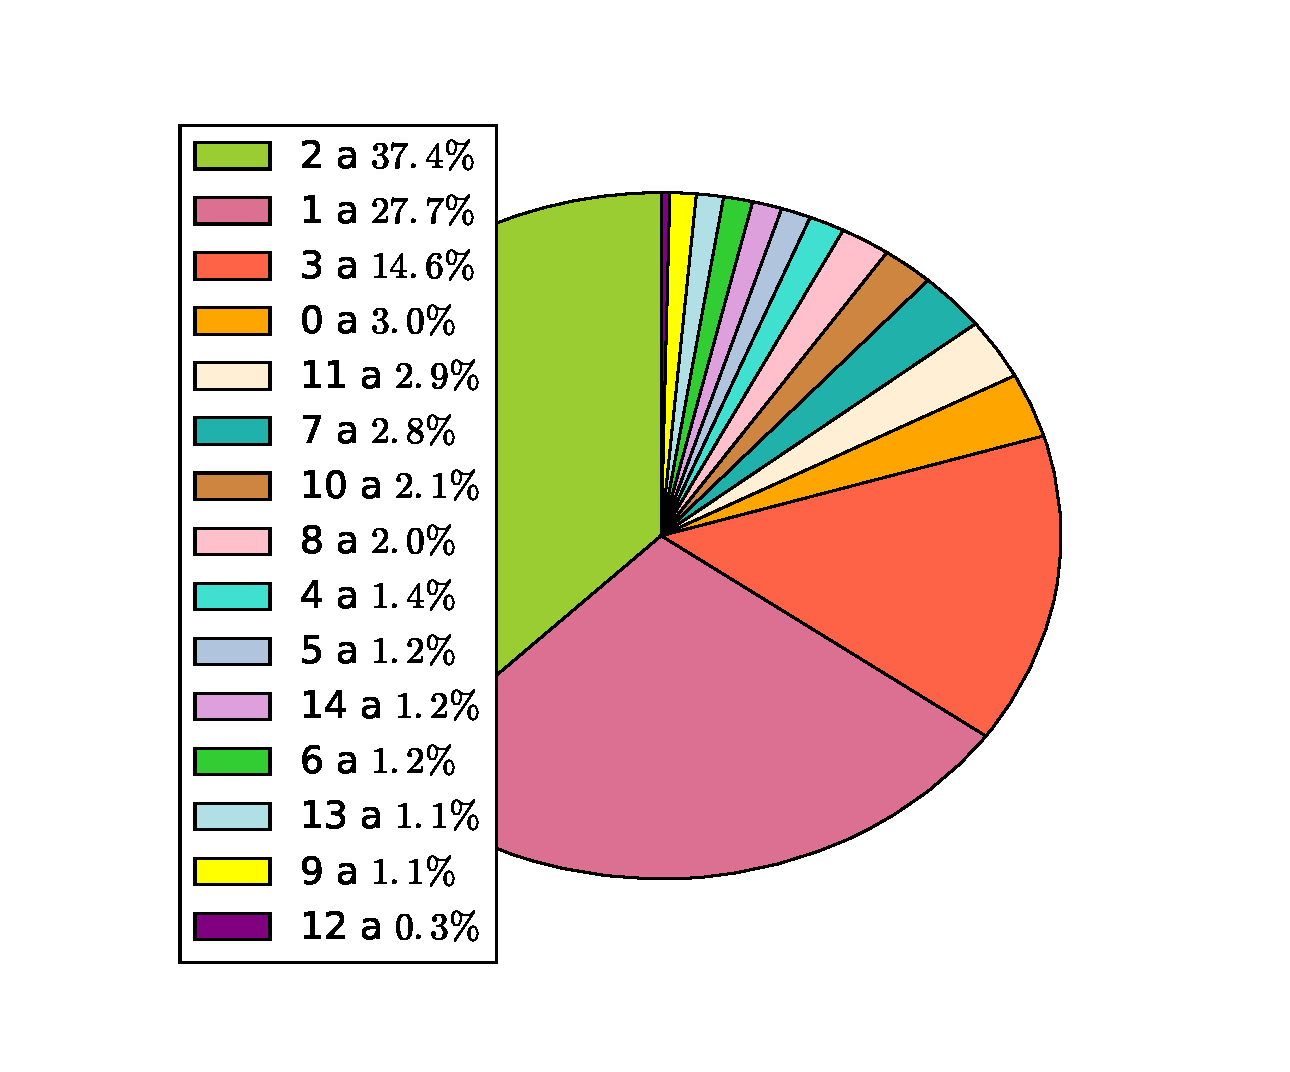
\includegraphics[width=\textwidth]{vanus_hoidja_sonad}
    \caption{hoidja sõnade vanuseline jaotumine kogu korpuses}
\end{figure}



\newpage

\section{Morfoloogiliselt märgendatud lapsekeele korpus}

\subsection{Tööprotsess}

Magistritöö eesmärk on luua eesti morfoloogiliselt märgendatud lapsekeele korpus, kuhu on koondatud kõik CHILDES-i eesti keele alamkorpused. Esialgne plaan oli konverteerida omalkäel kõik CHAT-failid XML-kujule, kuid sellega tekkisid mõningad tagasilöögid. Selleks, et CHAT-faile XML-kujule konverteerida, oleks tarvis, et kõik alamkorpused oleksid ühtsel kujul transkribeeritud ja kodeeritud. Peatükis 5.4 tõin välja mõned näited sellest, kui ebajärjepidevalt on seda tehtud. Isegi, kui korpused oleksid olnud standardsel kujul, siis oleks konverteerimisskripti tegemine muutunud väga keeruliseks ja ülejõukäivaks ülesandeks. Põhjus seisneb selles, et CHAT-käsiraamatus on väga suur ja lai valik kodeeringuid, mida on paraku ühel inimesel raske hallata. Näide (5) illustreerib seda, kuidas juba üsna lühikeses transkriptsiooni lõigus võib kodeeringute kasutus väga mitmekesine olla (kodeeringu seletus paikneb lausungi järel).

(5)
\begin{description}
    \item*CHI:   see kifiir \textbf{[:} kefiir\textbf{]} . | \emph{asendus}
    \item*MOT:   kus sa $\pmb{+/}$. | \emph{vahele segamine}
    \item*CHI:   $\pmb{+<}$ \textbf{(}h\textbf{)}akkas põlema . | \emph{pealerääkimine}, \emph{mittetäielik sõna}
    \item*MOT:   see ei ole kefiir ju .
    \item*CHI:   kefiir . $\pmb{[+}$ sr\textbf{]} | \emph{postcode}
    \item*MOT:   see on piim .
    \item*FAT:   mis see kook teeb ?
    \item*FAT:   tuleb ära panna $\pmb{[=}$ visata\textbf{]} või ? | \emph{seletus, tähendus}
    \item*MOT:   mina ei tea , vist jah .
    \item*CHI:   kuidas emme küpsetab saia , lihat\textbf{@n} \textbf{[*]} . | \emph{üleüldistamine}, \emph{vea markeerimine}
    \item\%err:   lihat=liha \$MOR
    \item*FAT:   saia ei ei küpseta .
    \item*FAT:   kartulit küpsetame , \textbf{(.)} ahjus . | \emph{paus}
    \item*CHI:   $\pmb{+<}$ saia . | \emph{pealerääkimine}
    \item*CHI:   lihat\textbf{@n} \textbf{[*]} . $\pmb{[+}$ \textbf{sr]} | \emph{postcode}
    \item\%err:   lihat=liha \$MOR
    \item*FAT:   liha ka jah .
    \item*CHI:   lihat\textbf{@n} \textbf{[*]} . $\pmb{[+}$ \textbf{sr]} | \emph{üleüldistamine}, \emph{vea markeerimine}, \emph{postcode}
    \item\%err:   lihat=liha \$MOR
    \item\%act:   MOT koorib sibulat
    \item...
    \item*CHI:   Atu \textbf{[:} Andreas\textbf{]} sõi $\pmb{+...}$ | \emph{asendus}, \emph{kõrvalekalle}
    \item*CHI:   $\pmb{+}$\textbf{"} a . | \emph{lausung jutumärkides}
    \item...
    \item*CHI:   käpad \textbf{(}h\textbf{)}aige \textbf{[*]} \textbf{[$\pmb{/]}$} käpad \textbf{(}h\textbf{)}aige \textbf{[*]} . | \emph{mittetäielik sõna}, \emph{vea markeerimine}, \emph{kordus}
    \item (Vija; 20018.cha)\\
\end{description}


On arusaadav, et iga uurija transkribeerib ja kodeerib lindistusi lähtuvalt enda eesmärkidest. Ühelt poolt on hea, et CHAT-käsiraamatus on niivõrd detailne kodeering, kuid teisalt võib selles orienteerumine vägagi raskeks osutuda. Kuna sellise konverteerimisskripti kirjutamise töömaht oleks selle magistritöö kirjutamise jaoks liiga töömahukaks osutunud, siis tuli leida uus lahendus. Korpuse tegemiseks vajalik keelematerjal pärineb samuti CHILDES-i andmebaasist, kuid need on juba eelnevalt CHAT-kujult XML-kujule konverteeritud failid. Aga kuna selle töö eesmärk on luua morfoloogiliselt märgendatud korpus, siis tuleb nendele XML-failidele ka lisada morfoloogiline tasand, mida neis failides ei ole. Selleks oli tarvis lähemalt tutvuda Talkbanki XML-skeema süntaksiga.


On arusaadav, et iga uurija transkribeerib ja kodeerib lindistusi lähtuvalt enda eesmärkidest. Ühelt poolt on hea, et CHAT-käsiraamatus on niivõrd detailne kodeering, kuid teisalt võib selles orienteerumine vägagi raskeks osutuda. Kuna sellise konverteerimisskripti kirjutamise töömaht oleks selle magistritöö kirjutamise jaoks liiga töömahukaks osutunud, siis tuli leida uus lahendus. Korpuse tegemiseks vajalik keelematerjal pärineb samuti CHILDES-i andmebaasist, kuid need on juba eelnevalt CHAT-kujult XML-kujule konverteeritud failid. Aga kuna selle töö eesmärk on luua morfoloogiliselt märgendatud korpus, siis tuleb nendele XML-failidele ka lisada morfoloogiline tasand, mida neis failides ei ole. Selleks oli tarvis lähemalt tutvuda \emph{Talkbank}i XML-skeema süntaksiga.

\subsubsection{\emph{Talkbank}i skeema}

Joonisel 2 on kujutatud minu töö seisukohalt olulisimad skeema elemendid.

\begin{figure}[H]
    \centering
    \includegraphics[width=10cm]{tag_elemendid}
    \caption{Talkbanki skeema elemendid}
\end{figure}

Talkbanki skeema juurelement on \emph{<CHAT>}, mille alluvad on \emph{<comment>}, \emph{<Participants>} ja \emph{<u>}. Elemendi \emph{<Participants>} alluv on \emph{<participant>}. \emph{<participant>} elemendis peitub metainfo lindistuse osalejate kohta (kõneleja ID, nimi, roll, keel, vanus ja sugu). Element \emph{<comment>} talletab metainfot lindistuse konteksti kohta (nt koht, kuupäev, lindistuse algus ja lõpp jne).

Näide (6) (Argus; hend10.xml)
\begin{lstlisting}
  <Participants>
    <participant
      id="CHI"
      name="Hendrik"
      role="Target_Child"
      language="est"
      age="P2Y2M6D"/>
    <participant
      id="EMA"
      role="Mother"
      language="est"/>
  </Participants>
  <comment type="Date">02-JUN-1997</comment>
\end{lstlisting}

Element \emph{<u>} tähistab kõneleja lausungit, selle kohustuslikeks atribuutideks on kõneleja ID ja lausungi järjekorra ID. \emph{<u>}-elemendil on palju alluvaid, aga selle töö juures osutusid olulisimateks \emph{<w>} ja \emph{<g>}. Element \emph{<w>} tähistab sõna ja \emph{<g>} sõnade gruppi. \emph{<g>} alluvaks võib olla tema ise või \emph{<w>}. Elemendi \emph{<w>} alluvaks võib olla \emph{<replacement>}. See element tähistab neid üksuseid, mida CHAT-käsiraamatu järgi kodeeritakse [: text] abil (vt näide (5) kifiir [: kefiir]), vt näide (7).\\

Näide (7) (Kohler; car030900.xml)
\begin{lstlisting}
  <u who='CHI' uID='u58'>
    <w>ehitame</w>
    <w>galaasi<replacement><w>garaazhi</w></replacement></w>
    <t type='p'></t>
  </u>
\end{lstlisting}

Morfoloogilise tasandi lisamine algab elemendiga \emph{<mor>}, mille alluv on \emph{<mw>} ehk \emph{morphemicWordType}. See jaguneb elemendiks \emph{<pos>} ja \emph{<stem>}. \emph{<pos>} tähistab sõnaliiki (ingl k. \emph{part of speech}). Selle alluvaks on \emph{<c>} ehk sõna morfoloogiline kategooria, mille sisuks on mittetühi string. Element \emph{<stem>} tähistab sõnatüve, mille sisuks on samuti mittetühi string.

\subsubsection{Morfoloogilise info lisamine}

\begin{figure}[H]
    \centering
    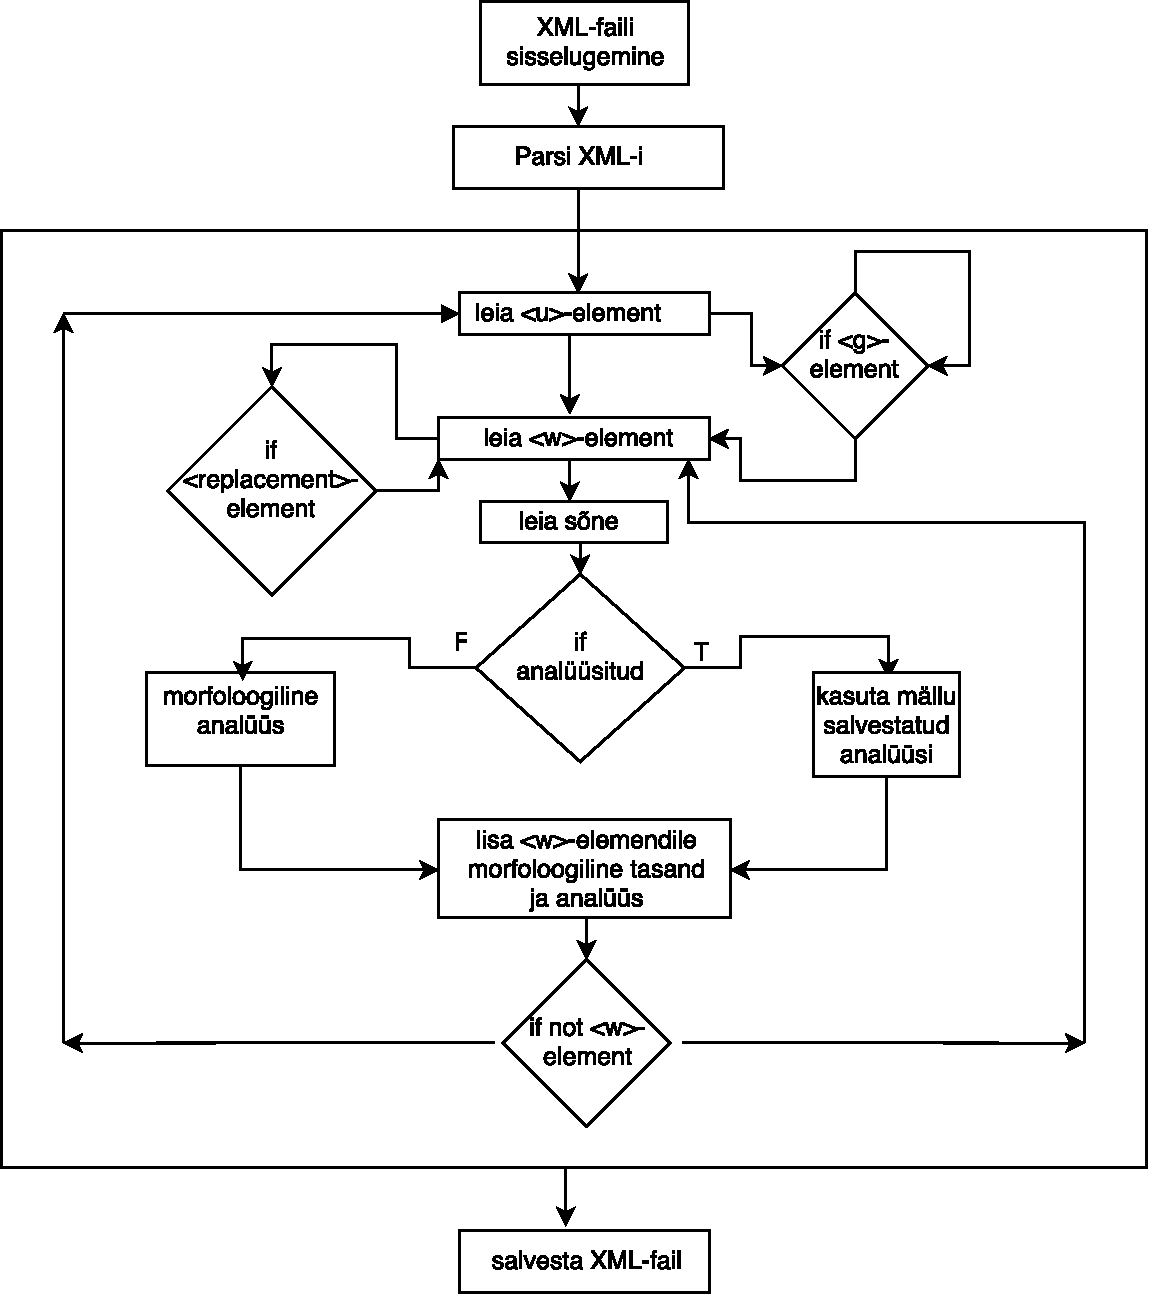
\includegraphics[width=12cm]{toovoog}
    \caption{Töövoog}
\end{figure}


Programmi kirjutamiseks on kasutatud Python 3.4 versiooni. Töövoog (vt joonis 3) on jaotatud 4 suuremaks osaks: XML-failide sisselugemine, faili parsimine, töötlemine ja modifitseeritud XML-faili salvestamine. Faili parsimiseks kasutan Pythoni moodulit \emph{ElementTree}, mis võimaldab lugeda ja genereerida XML hierarhiat. Parsimise käigus pannakse paika XML-faili juurelement ja sellele alluvad elemendid. Töötluse käigus navigeeritakse esmalt iga vestlusest osavõtja lausungi juurde. Seejärel leitakse kõik sõned ehk \emph{<w>}-elemendid. Juhul kui \emph{<w>}-elemendi alluv on element \emph{<replacement>}, siis uueks sõneks määratakse \emph{<replacement>}-elemendi \emph{<w>}-element.

Kui lausungi sõne on leitud, siis tehakse sõnele morfoloogiline analüüs. Morfoloogilise analüsaatorina kasutatakse \emph{etanat}. Sõne analüüs salvestatakse mällu, aga kui analüsaator saab sisendiks seni nägemata sõne (ehk mida mälus ei eksisteeri), siis tehakse sellele morfoloogiline analüüs. Põhjus seisneb programmi optimeerimises: morfoloogilise analüsaatori kutsumine iga sõne juures on üsna kulukas protsess. Seejärel lisatakse igale sõnele morfoloogiline tasand. Programm genereerib kirjutatud koodis järk-järgult puu elemendid ning morfoloogilisele tasandile jõudes hakkab sõne analüüse neile vastavatesse elementidesse lisama (vt joonis 2 ja näide (8)). Juhul kui sõne analüüse on rohkem kui üks, siis igale analüüsile genereeritakse uuesti morfoloogilise taseme elemendid. Samme korratakse seni, kuni jõutakse viimase lausungini ja lõpptulemus salvestatakse modifitseeritud XML-faili.

Näide (8) (Vija; 11120.xml)
\begin{lstlisting}
  <u uID="u7" who="CHI">
    <w>tuli
        <mor type="mor">
            <mw>
                <pos><c>_V_ Pers Prt Ind Sg3 Aff</c></pos>
                <stem>tule+i</stem>
            </mw>
        </mor>
        <mor type="mor">
            <mw>
                <pos><c>_S_ Sg Nom</c></pos>
                <stem>tuli+0</stem>
            </mw>
        </mor>
    </w>
    ...
\end{lstlisting}

\subsection{Morfoloogilise märgenduse hindamine}

Analüüsisin korpuseid morfoloogilist analüsaatorit kohandamata. Analüüsimisel ei teostatud oletamist ega ühestamist. Selle alapeatüki eesmärk on anda ülevaade sellest, kuidas jaotuvad analüüsi saanud ja tundmatuks jäänud sõnad igas vanuserühmas alamkorpuse kaupa.


\begin{table}[H]
\centering
\caption{Kõrgesaare korpus}
\resizebox{\textwidth}{!}{
\begin{tabular}{|l|c|c|c|c|c|c|}
\hline
vanus                  & \multicolumn{3}{c|}{lapse sõnad}                                                                                                                                                                                     & \multicolumn{3}{c|}{hoidja sõnad}                                                                                                                                                                                    \\ \hline
                       & \multicolumn{1}{l|}{analüüsitud}                                      & \multicolumn{1}{l|}{tundmatud}                                      & \multicolumn{1}{l|}{KOKKU}                                             & \multicolumn{1}{l|}{analüüsitud}                                      & \multicolumn{1}{l|}{tundmatud}                                      & \multicolumn{1}{l|}{KOKKU}                                             \\ \hline\hline
\multirow{2}{*}{1}     & \multirow{2}{*}{\begin{tabular}[c]{@{}c@{}}515\\ 47\%\end{tabular}}   & \multirow{2}{*}{\begin{tabular}[c]{@{}c@{}}575\\ 53\%\end{tabular}} & \multirow{2}{*}{\begin{tabular}[c]{@{}c@{}}1090\\ 100\%\end{tabular}}  & \multirow{2}{*}{\begin{tabular}[c]{@{}c@{}}11033\\ 93\%\end{tabular}} & \multirow{2}{*}{\begin{tabular}[c]{@{}c@{}}838\\ 7\%\end{tabular}}  & \multirow{2}{*}{\begin{tabular}[c]{@{}c@{}}11871\\ 100\%\end{tabular}} \\
                       &                                                                       &                                                                     &                                                                        &                                                                       &                                                                     &                                                                        \\ \hline
\multirow{2}{*}{2}     & \multirow{2}{*}{\begin{tabular}[c]{@{}c@{}}3208\\ 80\%\end{tabular}}  & \multirow{2}{*}{\begin{tabular}[c]{@{}c@{}}818\\ 20\%\end{tabular}} & \multirow{2}{*}{\begin{tabular}[c]{@{}c@{}}4026\\ 100\%\end{tabular}}  & \multirow{2}{*}{\begin{tabular}[c]{@{}c@{}}10030\\ 95\%\end{tabular}} & \multirow{2}{*}{\begin{tabular}[c]{@{}c@{}}534\\ 5\%\end{tabular}}  & \multirow{2}{*}{\begin{tabular}[c]{@{}c@{}}10564\\ 100\%\end{tabular}} \\
                       &                                                                       &                                                                     &                                                                        &                                                                       &                                                                     &                                                                        \\ \hline
\multirow{2}{*}{3}     & \multirow{2}{*}{\begin{tabular}[c]{@{}c@{}}2292\\ 90\%\end{tabular}}  & \multirow{2}{*}{\begin{tabular}[c]{@{}c@{}}242\\ 10\%\end{tabular}} & \multirow{2}{*}{\begin{tabular}[c]{@{}c@{}}2534\\ 100\%\end{tabular}}  & \multirow{2}{*}{\begin{tabular}[c]{@{}c@{}}5232\\ 94\%\end{tabular}}  & \multirow{2}{*}{\begin{tabular}[c]{@{}c@{}}319\\ 6\%\end{tabular}}  & \multirow{2}{*}{\begin{tabular}[c]{@{}c@{}}5551\\ 100\%\end{tabular}}  \\
                       &                                                                       &                                                                     &                                                                        &                                                                       &                                                                     &                                                                        \\ \hline
\multirow{2}{*}{4}     & \multirow{2}{*}{\begin{tabular}[c]{@{}c@{}}1439\\ 81\%\end{tabular}}  & \multirow{2}{*}{\begin{tabular}[c]{@{}c@{}}330\\ 19\%\end{tabular}} & \multirow{2}{*}{\begin{tabular}[c]{@{}c@{}}1769\\ 100\%\end{tabular}}  & \multirow{2}{*}{\begin{tabular}[c]{@{}c@{}}3929\\ 95\%\end{tabular}}  & \multirow{2}{*}{\begin{tabular}[c]{@{}c@{}}210\\ 5\%\end{tabular}}  & \multirow{2}{*}{\begin{tabular}[c]{@{}c@{}}4139\\ 100\%\end{tabular}}  \\
                       &                                                                       &                                                                     &                                                                        &                                                                       &                                                                     &                                                                        \\ \hline
\multirow{2}{*}{5}     & \multirow{2}{*}{\begin{tabular}[c]{@{}c@{}}2947\\ 91\%\end{tabular}}  & \multirow{2}{*}{\begin{tabular}[c]{@{}c@{}}309\\ 9\%\end{tabular}}  & \multirow{2}{*}{\begin{tabular}[c]{@{}c@{}}3256\\ 100\%\end{tabular}}  & \multirow{2}{*}{\begin{tabular}[c]{@{}c@{}}4531\\ 97\%\end{tabular}}  & \multirow{2}{*}{\begin{tabular}[c]{@{}c@{}}159\\ 3\%\end{tabular}}  & \multirow{2}{*}{\begin{tabular}[c]{@{}c@{}}4690\\ 100\%\end{tabular}}  \\
                       &                                                                       &                                                                     &                                                                        &                                                                       &                                                                     &                                                                        \\ \hline
\multirow{2}{*}{6}     & \multirow{2}{*}{\begin{tabular}[c]{@{}c@{}}3222\\ 94\%\end{tabular}}  & \multirow{2}{*}{\begin{tabular}[c]{@{}c@{}}213\\ 6\%\end{tabular}}  & \multirow{2}{*}{\begin{tabular}[c]{@{}c@{}}3435\\ 100\%\end{tabular}}  & \multirow{2}{*}{\begin{tabular}[c]{@{}c@{}}4435\\ 97\%\end{tabular}}  & \multirow{2}{*}{\begin{tabular}[c]{@{}c@{}}135\\ 3\%\end{tabular}}  & \multirow{2}{*}{\begin{tabular}[c]{@{}c@{}}4570\\ 100\%\end{tabular}}  \\
                       &                                                                       &                                                                     &                                                                        &                                                                       &                                                                     &                                                                        \\ \hline
\multirow{2}{*}{7}     & \multirow{2}{*}{\begin{tabular}[c]{@{}c@{}}7572\\ 94\%\end{tabular}}  & \multirow{2}{*}{\begin{tabular}[c]{@{}c@{}}518\\ 6\%\end{tabular}}  & \multirow{2}{*}{\begin{tabular}[c]{@{}c@{}}8090\\ 100\%\end{tabular}}  & \multirow{2}{*}{\begin{tabular}[c]{@{}c@{}}10489\\ 97\%\end{tabular}} & \multirow{2}{*}{\begin{tabular}[c]{@{}c@{}}278\\ 3\%\end{tabular}}  & \multirow{2}{*}{\begin{tabular}[c]{@{}c@{}}10767\\ 100\%\end{tabular}} \\
                       &                                                                       &                                                                     &                                                                        &                                                                       &                                                                     &                                                                        \\ \hline
\multirow{2}{*}{8}     & \multirow{2}{*}{\begin{tabular}[c]{@{}c@{}}5878\\ 94\%\end{tabular}}  & \multirow{2}{*}{\begin{tabular}[c]{@{}c@{}}400\\ 6\%\end{tabular}}  & \multirow{2}{*}{\begin{tabular}[c]{@{}c@{}}6278\\ 100\%\end{tabular}}  & \multirow{2}{*}{\begin{tabular}[c]{@{}c@{}}7522\\ 95\%\end{tabular}}  & \multirow{2}{*}{\begin{tabular}[c]{@{}c@{}}367\\ 5\%\end{tabular}}  & \multirow{2}{*}{\begin{tabular}[c]{@{}c@{}}7889\\ 100\%\end{tabular}}  \\
                       &                                                                       &                                                                     &                                                                        &                                                                       &                                                                     &                                                                        \\ \hline
\multirow{2}{*}{9}     & \multirow{2}{*}{\begin{tabular}[c]{@{}c@{}}3658\\ 93\%\end{tabular}}  & \multirow{2}{*}{\begin{tabular}[c]{@{}c@{}}269\\ 7\%\end{tabular}}  & \multirow{2}{*}{\begin{tabular}[c]{@{}c@{}}3927\\ 100\%\end{tabular}}  & \multirow{2}{*}{\begin{tabular}[c]{@{}c@{}}3879\\ 94\%\end{tabular}}  & \multirow{2}{*}{\begin{tabular}[c]{@{}c@{}}246\\ 6\%\end{tabular}}  & \multirow{2}{*}{\begin{tabular}[c]{@{}c@{}}4125\\ 100\%\end{tabular}}  \\
                       &                                                                       &                                                                     &                                                                        &                                                                       &                                                                     &                                                                        \\ \hline
\multirow{2}{*}{10}    & \multirow{2}{*}{\begin{tabular}[c]{@{}c@{}}7536\\ 94\%\end{tabular}}  & \multirow{2}{*}{\begin{tabular}[c]{@{}c@{}}518\\ 6\%\end{tabular}}  & \multirow{2}{*}{\begin{tabular}[c]{@{}c@{}}8054\\ 100\%\end{tabular}}  & \multirow{2}{*}{\begin{tabular}[c]{@{}c@{}}7717\\ 95\%\end{tabular}}  & \multirow{2}{*}{\begin{tabular}[c]{@{}c@{}}378\\ 5\%\end{tabular}}  & \multirow{2}{*}{\begin{tabular}[c]{@{}c@{}}8095\\ 100\%\end{tabular}}  \\
                       &                                                                       &                                                                     &                                                                        &                                                                       &                                                                     &                                                                        \\ \hline
\multirow{2}{*}{11}    & \multirow{2}{*}{\begin{tabular}[c]{@{}c@{}}11240\\ 93\%\end{tabular}} & \multirow{2}{*}{\begin{tabular}[c]{@{}c@{}}851\\ 7\%\end{tabular}}  & \multirow{2}{*}{\begin{tabular}[c]{@{}c@{}}12091\\ 100\%\end{tabular}} & \multirow{2}{*}{\begin{tabular}[c]{@{}c@{}}10762\\ 96\%\end{tabular}} & \multirow{2}{*}{\begin{tabular}[c]{@{}c@{}}399\\ 4\%\end{tabular}}  & \multirow{2}{*}{\begin{tabular}[c]{@{}c@{}}11161\\ 100\%\end{tabular}} \\
                       &                                                                       &                                                                     &                                                                        &                                                                       &                                                                     &                                                                        \\ \hline
\multirow{2}{*}{12}    & \multirow{2}{*}{\begin{tabular}[c]{@{}c@{}}1847\\ 92\%\end{tabular}}  & \multirow{2}{*}{\begin{tabular}[c]{@{}c@{}}156\\ 8\%\end{tabular}}  & \multirow{2}{*}{\begin{tabular}[c]{@{}c@{}}2003\\ 100\%\end{tabular}}  & \multirow{2}{*}{\begin{tabular}[c]{@{}c@{}}1274\\ 95\%\end{tabular}}  & \multirow{2}{*}{\begin{tabular}[c]{@{}c@{}}70\\ 5\%\end{tabular}}   & \multirow{2}{*}{\begin{tabular}[c]{@{}c@{}}1344\\ 100\%\end{tabular}}  \\
                       &                                                                       &                                                                     &                                                                        &                                                                       &                                                                     &                                                                        \\ \hline
\multirow{2}{*}{13}    & \multirow{2}{*}{\begin{tabular}[c]{@{}c@{}}3798\\ 89\%\end{tabular}}  & \multirow{2}{*}{\begin{tabular}[c]{@{}c@{}}492\\ 11\%\end{tabular}} & \multirow{2}{*}{\begin{tabular}[c]{@{}c@{}}4290\\ 100\%\end{tabular}}  & \multirow{2}{*}{\begin{tabular}[c]{@{}c@{}}4062\\ 95\%\end{tabular}}  & \multirow{2}{*}{\begin{tabular}[c]{@{}c@{}}199\\ 5\%\end{tabular}}  & \multirow{2}{*}{\begin{tabular}[c]{@{}c@{}}4261\\ 100\%\end{tabular}}  \\
                       &                                                                       &                                                                     &                                                                        &                                                                       &                                                                     &                                                                        \\ \hline
\multirow{2}{*}{14}    & \multirow{2}{*}{\begin{tabular}[c]{@{}c@{}}4525\\ 91\%\end{tabular}}  & \multirow{2}{*}{\begin{tabular}[c]{@{}c@{}}451\\ 9\%\end{tabular}}  & \multirow{2}{*}{\begin{tabular}[c]{@{}c@{}}4976\\ 100\%\end{tabular}}  & \multirow{2}{*}{\begin{tabular}[c]{@{}c@{}}4318\\ 93\%\end{tabular}}  & \multirow{2}{*}{\begin{tabular}[c]{@{}c@{}}347\\ 7\%\end{tabular}}  & \multirow{2}{*}{\begin{tabular}[c]{@{}c@{}}4665\\ 100\%\end{tabular}}  \\
                       &                                                                       &                                                                     &                                                                        &                                                                       &                                                                     &                                                                        \\ \hline\hline
\multirow{2}{*}{KOKKU} & \multirow{2}{*}{\begin{tabular}[c]{@{}c@{}}59677\\ 91\%\end{tabular}} & \multirow{2}{*}{\begin{tabular}[c]{@{}c@{}}6142\\ 9\%\end{tabular}} & \multirow{2}{*}{\begin{tabular}[c]{@{}c@{}}65819\\ 100\%\end{tabular}} & \multirow{2}{*}{\begin{tabular}[c]{@{}c@{}}89213\\ 95\%\end{tabular}} & \multirow{2}{*}{\begin{tabular}[c]{@{}c@{}}4479\\ 5\%\end{tabular}} & \multirow{2}{*}{\begin{tabular}[c]{@{}c@{}}93692\\ 100\%\end{tabular}} \\
                       &                                                                       &                                                                     &                                                                        &                                                                       &                                                                     &                                                                        \\ \hline
\end{tabular}}
\end{table}


\begin{table}[H]
\centering
\caption{Kapaneni korpus}
\resizebox{\textwidth}{!}{
\begin{tabular}{|l|c|c|c|c|c|c|}
\hline
vanus                  & \multicolumn{3}{c|}{lapse sõnad}                                                                                                                                                                                      & \multicolumn{3}{c|}{hoidja sõnad}                                                                                                                                                                                    \\ \hline
                       & \multicolumn{1}{l|}{analüüsitud}                                      & \multicolumn{1}{l|}{tundmatud}                                       & \multicolumn{1}{l|}{KOKKU}                                             & \multicolumn{1}{l|}{analüüsitud}                                      & \multicolumn{1}{l|}{tundmatud}                                      & \multicolumn{1}{l|}{KOKKU}                                             \\ \hline\hline
\multirow{2}{*}{1}     & \multirow{2}{*}{\begin{tabular}[c]{@{}c@{}}5093\\ 70\%\end{tabular}}  & \multirow{2}{*}{\begin{tabular}[c]{@{}c@{}}2209\\ 30\%\end{tabular}} & \multirow{2}{*}{\begin{tabular}[c]{@{}c@{}}7302\\ 100\%\end{tabular}}  & \multirow{2}{*}{\begin{tabular}[c]{@{}c@{}}16584\\ 93\%\end{tabular}} & \multirow{2}{*}{\begin{tabular}[c]{@{}c@{}}1207\\ 7\%\end{tabular}} & \multirow{2}{*}{\begin{tabular}[c]{@{}c@{}}17791\\ 100\%\end{tabular}} \\
                       &                                                                       &                                                                      &                                                                        &                                                                       &                                                                     &                                                                        \\ \hline
\multirow{2}{*}{2}     & \multirow{2}{*}{\begin{tabular}[c]{@{}c@{}}5689\\ 83\%\end{tabular}}  & \multirow{2}{*}{\begin{tabular}[c]{@{}c@{}}1142\\ 17\%\end{tabular}} & \multirow{2}{*}{\begin{tabular}[c]{@{}c@{}}6831\\ 100\%\end{tabular}}  & \multirow{2}{*}{\begin{tabular}[c]{@{}c@{}}9248\\ 94\%\end{tabular}}  & \multirow{2}{*}{\begin{tabular}[c]{@{}c@{}}583\\ 6\%\end{tabular}}  & \multirow{2}{*}{\begin{tabular}[c]{@{}c@{}}9831\\ 100\%\end{tabular}}  \\
                       &                                                                       &                                                                      &                                                                        &                                                                       &                                                                     &                                                                        \\ \hline
\multirow{2}{*}{3}     & \multirow{2}{*}{\begin{tabular}[c]{@{}c@{}}1601\\ 89\%\end{tabular}}  & \multirow{2}{*}{\begin{tabular}[c]{@{}c@{}}204\\ 11\%\end{tabular}}  & \multirow{2}{*}{\begin{tabular}[c]{@{}c@{}}1805\\ 100\%\end{tabular}}  & \multirow{2}{*}{\begin{tabular}[c]{@{}c@{}}2067\\ 98\%\end{tabular}}  & \multirow{2}{*}{\begin{tabular}[c]{@{}c@{}}48\\ 2\%\end{tabular}}   & \multirow{2}{*}{\begin{tabular}[c]{@{}c@{}}2115\\ 100\%\end{tabular}}  \\
                       &                                                                       &                                                                      &                                                                        &                                                                       &                                                                     &                                                                        \\ \hline\hline
\multirow{2}{*}{KOKKU} & \multirow{2}{*}{\begin{tabular}[c]{@{}c@{}}12383\\ 78\%\end{tabular}} & \multirow{2}{*}{\begin{tabular}[c]{@{}c@{}}3555\\ 22\%\end{tabular}} & \multirow{2}{*}{\begin{tabular}[c]{@{}c@{}}15938\\ 100\%\end{tabular}} & \multirow{2}{*}{\begin{tabular}[c]{@{}c@{}}27899\\ 94\%\end{tabular}} & \multirow{2}{*}{\begin{tabular}[c]{@{}c@{}}1838\\ 6\%\end{tabular}} & \multirow{2}{*}{\begin{tabular}[c]{@{}c@{}}29737\\ 100\%\end{tabular}} \\
                       &                                                                       &                                                                      &                                                                        &                                                                       &                                                                     &                                                                        \\ \hline
\end{tabular}}
\end{table}


\begin{table}[H]
\centering
\caption{Beeki korpus}
\resizebox{\textwidth}{!}{
\begin{tabular}{|l|c|c|c|c|c|c|}
\hline
vanus                  & \multicolumn{3}{c|}{lapse sõnad}                                                                                                                                                                                     & \multicolumn{3}{c|}{hoidja sõnad}                                                                                                                                                                                     \\ \hline
                       & \multicolumn{1}{l|}{analüüsitud}                                     & \multicolumn{1}{l|}{tundmatud}                                       & \multicolumn{1}{l|}{KOKKU}                                             & \multicolumn{1}{l|}{analüüsitud}                                      & \multicolumn{1}{l|}{tundmatud}                                       & \multicolumn{1}{l|}{KOKKU}                                             \\ \hline\hline
\multirow{2}{*}{0}     & \multirow{2}{*}{\begin{tabular}[c]{@{}c@{}}455\\ 31\%\end{tabular}}  & \multirow{2}{*}{\begin{tabular}[c]{@{}c@{}}995\\ 69\%\end{tabular}}  & \multirow{2}{*}{\begin{tabular}[c]{@{}c@{}}1450\\ 100\%\end{tabular}}  & \multirow{2}{*}{\begin{tabular}[c]{@{}c@{}}10282\\ 90\%\end{tabular}} & \multirow{2}{*}{\begin{tabular}[c]{@{}c@{}}1205\\ 10\%\end{tabular}} & \multirow{2}{*}{\begin{tabular}[c]{@{}c@{}}11487\\ 100\%\end{tabular}} \\
                       &                                                                      &                                                                      &                                                                        &                                                                       &                                                                      &                                                                        \\ \hline
\multirow{2}{*}{1}     & \multirow{2}{*}{\begin{tabular}[c]{@{}c@{}}297\\ 26\%\end{tabular}}  & \multirow{2}{*}{\begin{tabular}[c]{@{}c@{}}846\\ 74\%\end{tabular}}  & \multirow{2}{*}{\begin{tabular}[c]{@{}c@{}}1143\\ 100\%\end{tabular}}  & \multirow{2}{*}{\begin{tabular}[c]{@{}c@{}}9605\\ 92\%\end{tabular}}  & \multirow{2}{*}{\begin{tabular}[c]{@{}c@{}}858\\ 8\%\end{tabular}}   & \multirow{2}{*}{\begin{tabular}[c]{@{}c@{}}10463\\ 100\%\end{tabular}} \\
                       &                                                                      &                                                                      &                                                                        &                                                                       &                                                                      &                                                                        \\ \hline
\multirow{2}{*}{2}     & \multirow{2}{*}{\begin{tabular}[c]{@{}c@{}}5034\\ 66\%\end{tabular}} & \multirow{2}{*}{\begin{tabular}[c]{@{}c@{}}2537\\ 34\%\end{tabular}} & \multirow{2}{*}{\begin{tabular}[c]{@{}c@{}}7571\\ 100\%\end{tabular}}  & \multirow{2}{*}{\begin{tabular}[c]{@{}c@{}}25196\\ 93\%\end{tabular}} & \multirow{2}{*}{\begin{tabular}[c]{@{}c@{}}1826\\ 7\%\end{tabular}}  & \multirow{2}{*}{\begin{tabular}[c]{@{}c@{}}27022\\ 100\%\end{tabular}} \\
                       &                                                                      &                                                                      &                                                                        &                                                                       &                                                                      &                                                                        \\ \hline\hline
\multirow{2}{*}{KOKKU} & \multirow{2}{*}{\begin{tabular}[c]{@{}c@{}}5786\\ 57\%\end{tabular}} & \multirow{2}{*}{\begin{tabular}[c]{@{}c@{}}4378\\ 43\%\end{tabular}} & \multirow{2}{*}{\begin{tabular}[c]{@{}c@{}}10164\\ 100\%\end{tabular}} & \multirow{2}{*}{\begin{tabular}[c]{@{}c@{}}45083\\ 92\%\end{tabular}} & \multirow{2}{*}{\begin{tabular}[c]{@{}c@{}}3889\\ 8\%\end{tabular}}  & \multirow{2}{*}{\begin{tabular}[c]{@{}c@{}}48972\\ 100\%\end{tabular}} \\
                       &                                                                      &                                                                      &                                                                        &                                                                       &                                                                      &                                                                        \\ \hline
\end{tabular}}
\end{table}


\begin{table}[H]
\centering
\caption{Kohleri korpus}
\resizebox{\textwidth}{!}{
\begin{tabular}{|l|c|c|c|c|c|c|}
\hline
vanus                  & \multicolumn{3}{c|}{lapse sõnad}                                                                                                                                                                                   & \multicolumn{3}{c|}{hoidja sõnad}                                                                                                                                                                                    \\ \hline
                       & \multicolumn{1}{l|}{analüüsitud}                                     & \multicolumn{1}{l|}{tundmatud}                                     & \multicolumn{1}{l|}{KOKKU}                                             & \multicolumn{1}{l|}{analüüsitud}                                      & \multicolumn{1}{l|}{tundmatud}                                      & \multicolumn{1}{l|}{KOKKU}                                             \\ \hline\hline
\multirow{2}{*}{0}     & \multirow{2}{*}{\begin{tabular}[c]{@{}c@{}}6\\ 100\%\end{tabular}}   & \multirow{2}{*}{\begin{tabular}[c]{@{}c@{}}0\\ 0\%\end{tabular}}   & \multirow{2}{*}{\begin{tabular}[c]{@{}c@{}}6\\ 100\%\end{tabular}}     & \multirow{2}{*}{\begin{tabular}[c]{@{}c@{}}281\\ 95\%\end{tabular}}   & \multirow{2}{*}{\begin{tabular}[c]{@{}c@{}}14\\ 5\%\end{tabular}}   & \multirow{2}{*}{\begin{tabular}[c]{@{}c@{}}295\\ 100\%\end{tabular}}   \\
                       &                                                                      &                                                                    &                                                                        &                                                                       &                                                                     &                                                                        \\ \hline
\multirow{2}{*}{1}     & \multirow{2}{*}{\begin{tabular}[c]{@{}c@{}}4592\\ 93\%\end{tabular}} & \multirow{2}{*}{\begin{tabular}[c]{@{}c@{}}348\\ 7\%\end{tabular}} & \multirow{2}{*}{\begin{tabular}[c]{@{}c@{}}4940\\ 100\%\end{tabular}}  & \multirow{2}{*}{\begin{tabular}[c]{@{}c@{}}40724\\ 97\%\end{tabular}} & \multirow{2}{*}{\begin{tabular}[c]{@{}c@{}}1160\\ 3\%\end{tabular}} & \multirow{2}{*}{\begin{tabular}[c]{@{}c@{}}41884\\ 100\%\end{tabular}} \\
                       &                                                                      &                                                                    &                                                                        &                                                                       &                                                                     &                                                                        \\ \hline
\multirow{2}{*}{2}     & \multirow{2}{*}{\begin{tabular}[c]{@{}c@{}}4992\\ 98\%\end{tabular}} & \multirow{2}{*}{\begin{tabular}[c]{@{}c@{}}115\\ 2\%\end{tabular}} & \multirow{2}{*}{\begin{tabular}[c]{@{}c@{}}5107\\ 100\%\end{tabular}}  & \multirow{2}{*}{\begin{tabular}[c]{@{}c@{}}18224\\ 99\%\end{tabular}} & \multirow{2}{*}{\begin{tabular}[c]{@{}c@{}}256\\ 1\%\end{tabular}}  & \multirow{2}{*}{\begin{tabular}[c]{@{}c@{}}18480\\ 100\%\end{tabular}} \\
                       &                                                                      &                                                                    &                                                                        &                                                                       &                                                                     &                                                                        \\ \hline\hline
\multirow{2}{*}{KOKKU} & \multirow{2}{*}{\begin{tabular}[c]{@{}c@{}}9590\\ 95\%\end{tabular}} & \multirow{2}{*}{\begin{tabular}[c]{@{}c@{}}463\\ 5\%\end{tabular}} & \multirow{2}{*}{\begin{tabular}[c]{@{}c@{}}10053\\ 100\%\end{tabular}} & \multirow{2}{*}{\begin{tabular}[c]{@{}c@{}}59229\\ 98\%\end{tabular}} & \multirow{2}{*}{\begin{tabular}[c]{@{}c@{}}1430\\ 2\%\end{tabular}} & \multirow{2}{*}{\begin{tabular}[c]{@{}c@{}}60659\\ 100\%\end{tabular}} \\
                       &                                                                      &                                                                    &                                                                        &                                                                       &                                                                     &                                                                        \\ \hline
\end{tabular}}
\end{table}



\begin{table}[H]
\centering
\caption{Vija korpus}
\resizebox{\textwidth}{!}{
\begin{tabular}{|l|c|c|c|c|c|c|}
\hline
vanus                  & \multicolumn{3}{c|}{lapse sõnad}                                                                                                                                                                                       & \multicolumn{3}{c|}{hoidja sõnad}                                                                                                                                                                                      \\ \hline
                       & \multicolumn{1}{l|}{analüüsitud}                                       & \multicolumn{1}{l|}{tundmatud}                                      & \multicolumn{1}{l|}{KOKKU}                                              & \multicolumn{1}{l|}{analüüsitud}                                       & \multicolumn{1}{l|}{tundmatud}                                      & \multicolumn{1}{l|}{KOKKU}                                              \\ \hline\hline
\multirow{2}{*}{1}     & \multirow{2}{*}{\begin{tabular}[c]{@{}c@{}}2213\\ 78\%\end{tabular}}   & \multirow{2}{*}{\begin{tabular}[c]{@{}c@{}}632\\ 22\%\end{tabular}} & \multirow{2}{*}{\begin{tabular}[c]{@{}c@{}}2845\\ 100\%\end{tabular}}   & \multirow{2}{*}{\begin{tabular}[c]{@{}c@{}}8391\\ 98\%\end{tabular}}   & \multirow{2}{*}{\begin{tabular}[c]{@{}c@{}}130\\ 2\%\end{tabular}}  & \multirow{2}{*}{\begin{tabular}[c]{@{}c@{}}8521\\ 100\%\end{tabular}}   \\
                       &                                                                        &                                                                     &                                                                         &                                                                        &                                                                     &                                                                         \\ \hline
\multirow{2}{*}{2}     & \multirow{2}{*}{\begin{tabular}[c]{@{}c@{}}39313\\ 95\%\end{tabular}}  & \multirow{2}{*}{\begin{tabular}[c]{@{}c@{}}2185\\ 5\%\end{tabular}} & \multirow{2}{*}{\begin{tabular}[c]{@{}c@{}}41498\\ 100\%\end{tabular}}  & \multirow{2}{*}{\begin{tabular}[c]{@{}c@{}}57989\\ 98\%\end{tabular}}  & \multirow{2}{*}{\begin{tabular}[c]{@{}c@{}}1283\\ 2\%\end{tabular}} & \multirow{2}{*}{\begin{tabular}[c]{@{}c@{}}59272\\ 100\%\end{tabular}}  \\
                       &                                                                        &                                                                     &                                                                         &                                                                        &                                                                     &                                                                         \\ \hline
\multirow{2}{*}{3}     & \multirow{2}{*}{\begin{tabular}[c]{@{}c@{}}64231\\ 97\%\end{tabular}}  & \multirow{2}{*}{\begin{tabular}[c]{@{}c@{}}1807\\ 3\%\end{tabular}} & \multirow{2}{*}{\begin{tabular}[c]{@{}c@{}}66038\\ 100\%\end{tabular}}  & \multirow{2}{*}{\begin{tabular}[c]{@{}c@{}}47466\\ 99\%\end{tabular}}  & \multirow{2}{*}{\begin{tabular}[c]{@{}c@{}}671\\ 1\%\end{tabular}}  & \multirow{2}{*}{\begin{tabular}[c]{@{}c@{}}48137\\ 100\%\end{tabular}}  \\
                       &                                                                        &                                                                     &                                                                         &                                                                        &                                                                     &                                                                         \\ \hline\hline
\multirow{2}{*}{KOKKU} & \multirow{2}{*}{\begin{tabular}[c]{@{}c@{}}105757\\ 96\%\end{tabular}} & \multirow{2}{*}{\begin{tabular}[c]{@{}c@{}}4624\\ 4\%\end{tabular}} & \multirow{2}{*}{\begin{tabular}[c]{@{}c@{}}110381\\ 100\%\end{tabular}} & \multirow{2}{*}{\begin{tabular}[c]{@{}c@{}}113846\\ 98\%\end{tabular}} & \multirow{2}{*}{\begin{tabular}[c]{@{}c@{}}2084\\ 2\%\end{tabular}} & \multirow{2}{*}{\begin{tabular}[c]{@{}c@{}}115930\\ 100\%\end{tabular}} \\
                       &                                                                        &                                                                     &                                                                         &                                                                        &                                                                     &                                                                         \\ \hline
\end{tabular}}
\end{table}


\begin{table}[H]
\centering
\caption{Arguse korpus}
\resizebox{\textwidth}{!}{
\begin{tabular}{|l|c|c|c|c|c|c|}
\hline
vanus                  & \multicolumn{3}{c|}{lapse sõnad}                                                                                                                                                                                   & \multicolumn{3}{c|}{hoidja sõnad}                                                                                                                                                                                 \\ \hline
                       & \multicolumn{1}{l|}{analüüsitud}                                     & \multicolumn{1}{l|}{tundmatud}                                      & \multicolumn{1}{l|}{KOKKU}                                            & \multicolumn{1}{l|}{analüüsitud}                                     & \multicolumn{1}{l|}{tundmatud}                                     & \multicolumn{1}{l|}{KOKKU}                                            \\ \hline\hline
\multirow{2}{*}{1}     & \multirow{2}{*}{\begin{tabular}[c]{@{}c@{}}361\\ 64\%\end{tabular}}  & \multirow{2}{*}{\begin{tabular}[c]{@{}c@{}}205\\ 36\%\end{tabular}} & \multirow{2}{*}{\begin{tabular}[c]{@{}c@{}}566\\ 100\%\end{tabular}}  & \multirow{2}{*}{\begin{tabular}[c]{@{}c@{}}1884\\ 96\%\end{tabular}} & \multirow{2}{*}{\begin{tabular}[c]{@{}c@{}}79\\ 4\%\end{tabular}}  & \multirow{2}{*}{\begin{tabular}[c]{@{}c@{}}1963\\ 100\%\end{tabular}} \\
                       &                                                                      &                                                                     &                                                                       &                                                                      &                                                                    &                                                                       \\ \hline
\multirow{2}{*}{2}     & \multirow{2}{*}{\begin{tabular}[c]{@{}c@{}}3092\\ 85\%\end{tabular}} & \multirow{2}{*}{\begin{tabular}[c]{@{}c@{}}562\\ 15\%\end{tabular}} & \multirow{2}{*}{\begin{tabular}[c]{@{}c@{}}3654\\ 100\%\end{tabular}} & \multirow{2}{*}{\begin{tabular}[c]{@{}c@{}}6945\\ 97\%\end{tabular}} & \multirow{2}{*}{\begin{tabular}[c]{@{}c@{}}245\\ 3\%\end{tabular}} & \multirow{2}{*}{\begin{tabular}[c]{@{}c@{}}7190\\ 100\%\end{tabular}} \\
                       &                                                                      &                                                                     &                                                                       &                                                                      &                                                                    &                                                                       \\ \hline\hline
\multirow{2}{*}{KOKKU} & \multirow{2}{*}{\begin{tabular}[c]{@{}c@{}}3453\\ 82\%\end{tabular}} & \multirow{2}{*}{\begin{tabular}[c]{@{}c@{}}767\\ 18\%\end{tabular}} & \multirow{2}{*}{\begin{tabular}[c]{@{}c@{}}4220\\ 100\%\end{tabular}} & \multirow{2}{*}{\begin{tabular}[c]{@{}c@{}}8829\\ 96\%\end{tabular}} & \multirow{2}{*}{\begin{tabular}[c]{@{}c@{}}324\\ 4\%\end{tabular}} & \multirow{2}{*}{\begin{tabular}[c]{@{}c@{}}9153\\ 100\%\end{tabular}} \\
                       &                                                                      &                                                                     &                                                                       &                                                                      &                                                                    &                                                                       \\ \hline
\end{tabular}}
\end{table}


\begin{table}[H]
\centering
\caption{Zuppingu korpus}
\resizebox{\textwidth}{!}{
\begin{tabular}{|l|c|c|c|c|c|c|}
\hline
vanus                  & \multicolumn{3}{c|}{lapse sõnad}                                                                                                                                                                                     & \multicolumn{3}{c|}{hoidja sõnad}                                                                                                                                                                                   \\ \hline
                       & \multicolumn{1}{l|}{analüüsitud}                                     & \multicolumn{1}{l|}{tundmatud}                                       & \multicolumn{1}{l|}{KOKKU}                                             & \multicolumn{1}{l|}{analüüsitud}                                      & \multicolumn{1}{l|}{tundmatud}                                     & \multicolumn{1}{l|}{KOKKU}                                             \\ \hline\hline
\multirow{2}{*}{1}     & \multirow{2}{*}{\begin{tabular}[c]{@{}c@{}}2508\\ 68\%\end{tabular}} & \multirow{2}{*}{\begin{tabular}[c]{@{}c@{}}1169\\ 32\%\end{tabular}} & \multirow{2}{*}{\begin{tabular}[c]{@{}c@{}}3677\\ 100\%\end{tabular}}  & \multirow{2}{*}{\begin{tabular}[c]{@{}c@{}}14756\\ 97\%\end{tabular}} & \multirow{2}{*}{\begin{tabular}[c]{@{}c@{}}435\\ 3\%\end{tabular}} & \multirow{2}{*}{\begin{tabular}[c]{@{}c@{}}15191\\ 100\%\end{tabular}} \\
                       &                                                                      &                                                                      &                                                                        &                                                                       &                                                                    &                                                                        \\ \hline
\multirow{2}{*}{2}     & \multirow{2}{*}{\begin{tabular}[c]{@{}c@{}}5782\\ 85\%\end{tabular}} & \multirow{2}{*}{\begin{tabular}[c]{@{}c@{}}1003\\ 15\%\end{tabular}} & \multirow{2}{*}{\begin{tabular}[c]{@{}c@{}}6785\\ 100\%\end{tabular}}  & \multirow{2}{*}{\begin{tabular}[c]{@{}c@{}}12882\\ 98\%\end{tabular}} & \multirow{2}{*}{\begin{tabular}[c]{@{}c@{}}232\\ 2\%\end{tabular}} & \multirow{2}{*}{\begin{tabular}[c]{@{}c@{}}13114\\ 100\%\end{tabular}} \\
                       &                                                                      &                                                                      &                                                                        &                                                                       &                                                                    &                                                                        \\ \hline
\multirow{2}{*}{3}     & \multirow{2}{*}{\begin{tabular}[c]{@{}c@{}}470\\ 87\%\end{tabular}}  & \multirow{2}{*}{\begin{tabular}[c]{@{}c@{}}72\\ 13\%\end{tabular}}   & \multirow{2}{*}{\begin{tabular}[c]{@{}c@{}}542\\ 100\%\end{tabular}}   & \multirow{2}{*}{\begin{tabular}[c]{@{}c@{}}1028\\ 98\%\end{tabular}}  & \multirow{2}{*}{\begin{tabular}[c]{@{}c@{}}24\\ 2\%\end{tabular}}  & \multirow{2}{*}{\begin{tabular}[c]{@{}c@{}}1052\\ 100\%\end{tabular}}  \\
                       &                                                                      &                                                                      &                                                                        &                                                                       &                                                                    &                                                                        \\ \hline
\multirow{2}{*}{4}     & \multirow{2}{*}{\begin{tabular}[c]{@{}c@{}}596\\ 95\%\end{tabular}}  & \multirow{2}{*}{\begin{tabular}[c]{@{}c@{}}32\\ 5\%\end{tabular}}    & \multirow{2}{*}{\begin{tabular}[c]{@{}c@{}}628\\ 100\%\end{tabular}}   & \multirow{2}{*}{\begin{tabular}[c]{@{}c@{}}1455\\ 99\%\end{tabular}}  & \multirow{2}{*}{\begin{tabular}[c]{@{}c@{}}17\\ 1\%\end{tabular}}  & \multirow{2}{*}{\begin{tabular}[c]{@{}c@{}}1472\\ 100\%\end{tabular}}  \\
                       &                                                                      &                                                                      &                                                                        &                                                                       &                                                                    &                                                                        \\ \hline\hline
\multirow{2}{*}{KOKKU} & \multirow{2}{*}{\begin{tabular}[c]{@{}c@{}}9356\\ 80\%\end{tabular}} & \multirow{2}{*}{\begin{tabular}[c]{@{}c@{}}2276\\ 20\%\end{tabular}} & \multirow{2}{*}{\begin{tabular}[c]{@{}c@{}}11632\\ 100\%\end{tabular}} & \multirow{2}{*}{\begin{tabular}[c]{@{}c@{}}30121\\ 98\%\end{tabular}} & \multirow{2}{*}{\begin{tabular}[c]{@{}c@{}}708\\ 2\%\end{tabular}} & \multirow{2}{*}{\begin{tabular}[c]{@{}c@{}}30829\\ 100\%\end{tabular}} \\
                       &                                                                      &                                                                      &                                                                        &                                                                       &                                                                    &                                                                        \\ \hline
\end{tabular}}
\end{table}

Võtame esmalt vaatluse alla hoidja sõnad. Tabelitest on näha, et nii analüüsi saanud kui ka tundmatuks jäänud sõnade osakaal igas korpuses on üsna stabiilselt jaotunud. Analüüsitud sõnade üldine osakaal igas korpuses varieerub 94\%--98\% vahel ja tundmatute sõnade osakaal 2\%--8\% vahel. Need tulemused on lootustäratavad, kuna tegemist on suulise keelega, mille erijooned võivad olla kirjakeele analüüsimiseks loodud morfoloogilise analüsaatori jaoks problemaatilised. Näiteks uue meedia keelekasutus on oma spontaansuse ja mitteformaalsuse tõttu sarnane suulisele keelele ja erineb kirjakeelest nii leksikoni kui ortograafia poolest. Uue meedia (ehk internetikeele) korpuste esmasel morfoloogilisel analüüsimisel saadi tundmatute sõnade protsendiks jututubades 27,2\%, foorumites 10.3\%, kommentaariumites 5,6\% ja uudisgruppides 11,7\% \citep{UUSMEEDIA}. Pärast kasutajasõnastiku ja eeltöötluse rakendamist vähenes tundmatute sõnade protsent jututubades 10,5\%, foorumites 8.8\%, kommentaariumites 4,8\% ja uudisgruppides 10,5\%-ni. Seega väike tundmatute sõnade \% hoidja keeles on hea, kuid need andmed võivad viidata ka sellele, et korpuse transkribeerijad on pannud hoidja keelt kirja kirjakeelele sarnaselt.

Lapse sõnade puhul varieerub analüüsitud sõnade üldine osakaal igas korpuses 57\%--96\% vahel ja tundmatud sõnad 4\%--43\% vahel. Kõige suurem tundmatute sõnade osakaal on Beeki korpuses (vt tabel 12). Seal varieerub tundmatute sõnade \% 34 ja 74 vahel. Beekile järgneb Kapaneni korpus (vt tabel 11), kus tundmatute sõnade \% varieerub 11 ja 30 vahel. Zuppingu korpuses (vt tabel 16) varieerub 5 ja 32\% vahel ning Arguse korpuses (vt tabel 15) 15 ja 36\% vahel. Kõige väiksem tundmatute sõnade osakaal on Vija (vt tabel 14) ja Kohleri korpuses (vt tabel 13). Vija korpuses varieerub tundmatute sõnade protsent 3 ja 22 vahel, kuid Kohleri korpuses 0 ja 7\% vahel. Kõrgesaare korpuses (vt tabel 10) varieerub tundmatute sõnade osakaal vahemikus 6\%--53\%. Olenemata sellest, et tundmatute sõnade \% amplituut on suur, jääb üldine skoor alla 10\%. Huvitav see, et kui teiste korpuste puhul üldjuhul vanuse suurenemisega kahaneb tundmatute sõnade osakaal, siis näiteks Kohleri korpuses 1. vanusegrupp ehk 0-aastaste puhul on tundmatuid sõnu 0\%. Sama on ka Beeki korpuses, kus 0-aastaste protsent on väiksem kui 1-aastaste seas (69\% vs 74\%).

Need andmed võivad viidata sellele, et tundmatute sõnade osakaal võib sõltuda paljuski transkribeerijast, täpsemalt transkribeerija üleskirjutamise viisist. Alamkorpuste standardiseerimise alapeatükis kirjutasin, et transkribeerija peab nägema ja teadma, mida lindistuses tegelikult öelda taheti, ja vastavad kodeeringud peaksid transkriptsioonis olema nii lisatud, et vead oleksid juba esimesel tasandil liigitatud.
Selleks, et morfoloogiline analüsaator saaks oma tööd hästi teha, oleks tarvis, et transkribeerijad kasutaksid üleskirjutamisel kodeeringut ([: sõna]), mis asendab kõneleja poolt produtseeritud sõna selle kirjakeelele vastava sõnaga. Näiteks vaatame Kohleri korpuses 1.vanusegruppi, kus tundmatute sõnade osakaal on 0\%. Analüüsitud sõnavorme on kokku 4:

\begin{table}[H]
\begin{tabular}{|l|l|l|}
\hline
lapse sõna & asendus & analüüs       \\ \hline\hline
teh        & tere    & \_I\_ tere+0  \\ \hline
tehe       & tere    & \_I\_ tere+0  \\ \hline
täh        & aitäh   & \_I\_ aitäh+0 \\ \hline
äh         & aitäh   & \_I\_ aitäh+0 \\ \hline
\end{tabular}
\end{table}

Me näeme, et kontekstita need sõnad justkui ei tähenda miskit, aga kuna nendele sõnadele on juurde lisatud kodeering selle kohta, mida need tegelikkuses tähendavad või mida laps üritas öelda, siis saab morfoloogiline analüsaaator oma tööga hästi hakkama ja seetõttu pole selle lapse keelekasutuses ühtki tundmatut sõna. Sel põhjusel annab alust arvata, et nii on ka teiste korpuste puhul.

Seni olen arutlenud vaid tundmatute sõnade teemal, kuid morfoloogilise analüsaatori adekvaatsuse hindamiseks tuleb vaatluse alla võtta ka analüüsi saanud sõnad. Selleks oli tarvis faile käsitsi läbi vaadata. Igast korpusest vailisin juhuslikkuse alusel ühe faili ja hindasin iga sõna puhul, kas saadud analüüs on õige või mitte. Joonisel 28 on kujutatud, kuidas jaotuvad iga alamkorpuse kaupa õige ja vale analüüsi saanud sõnad.
\hfill


\begin{figure}[H]
    \centering
    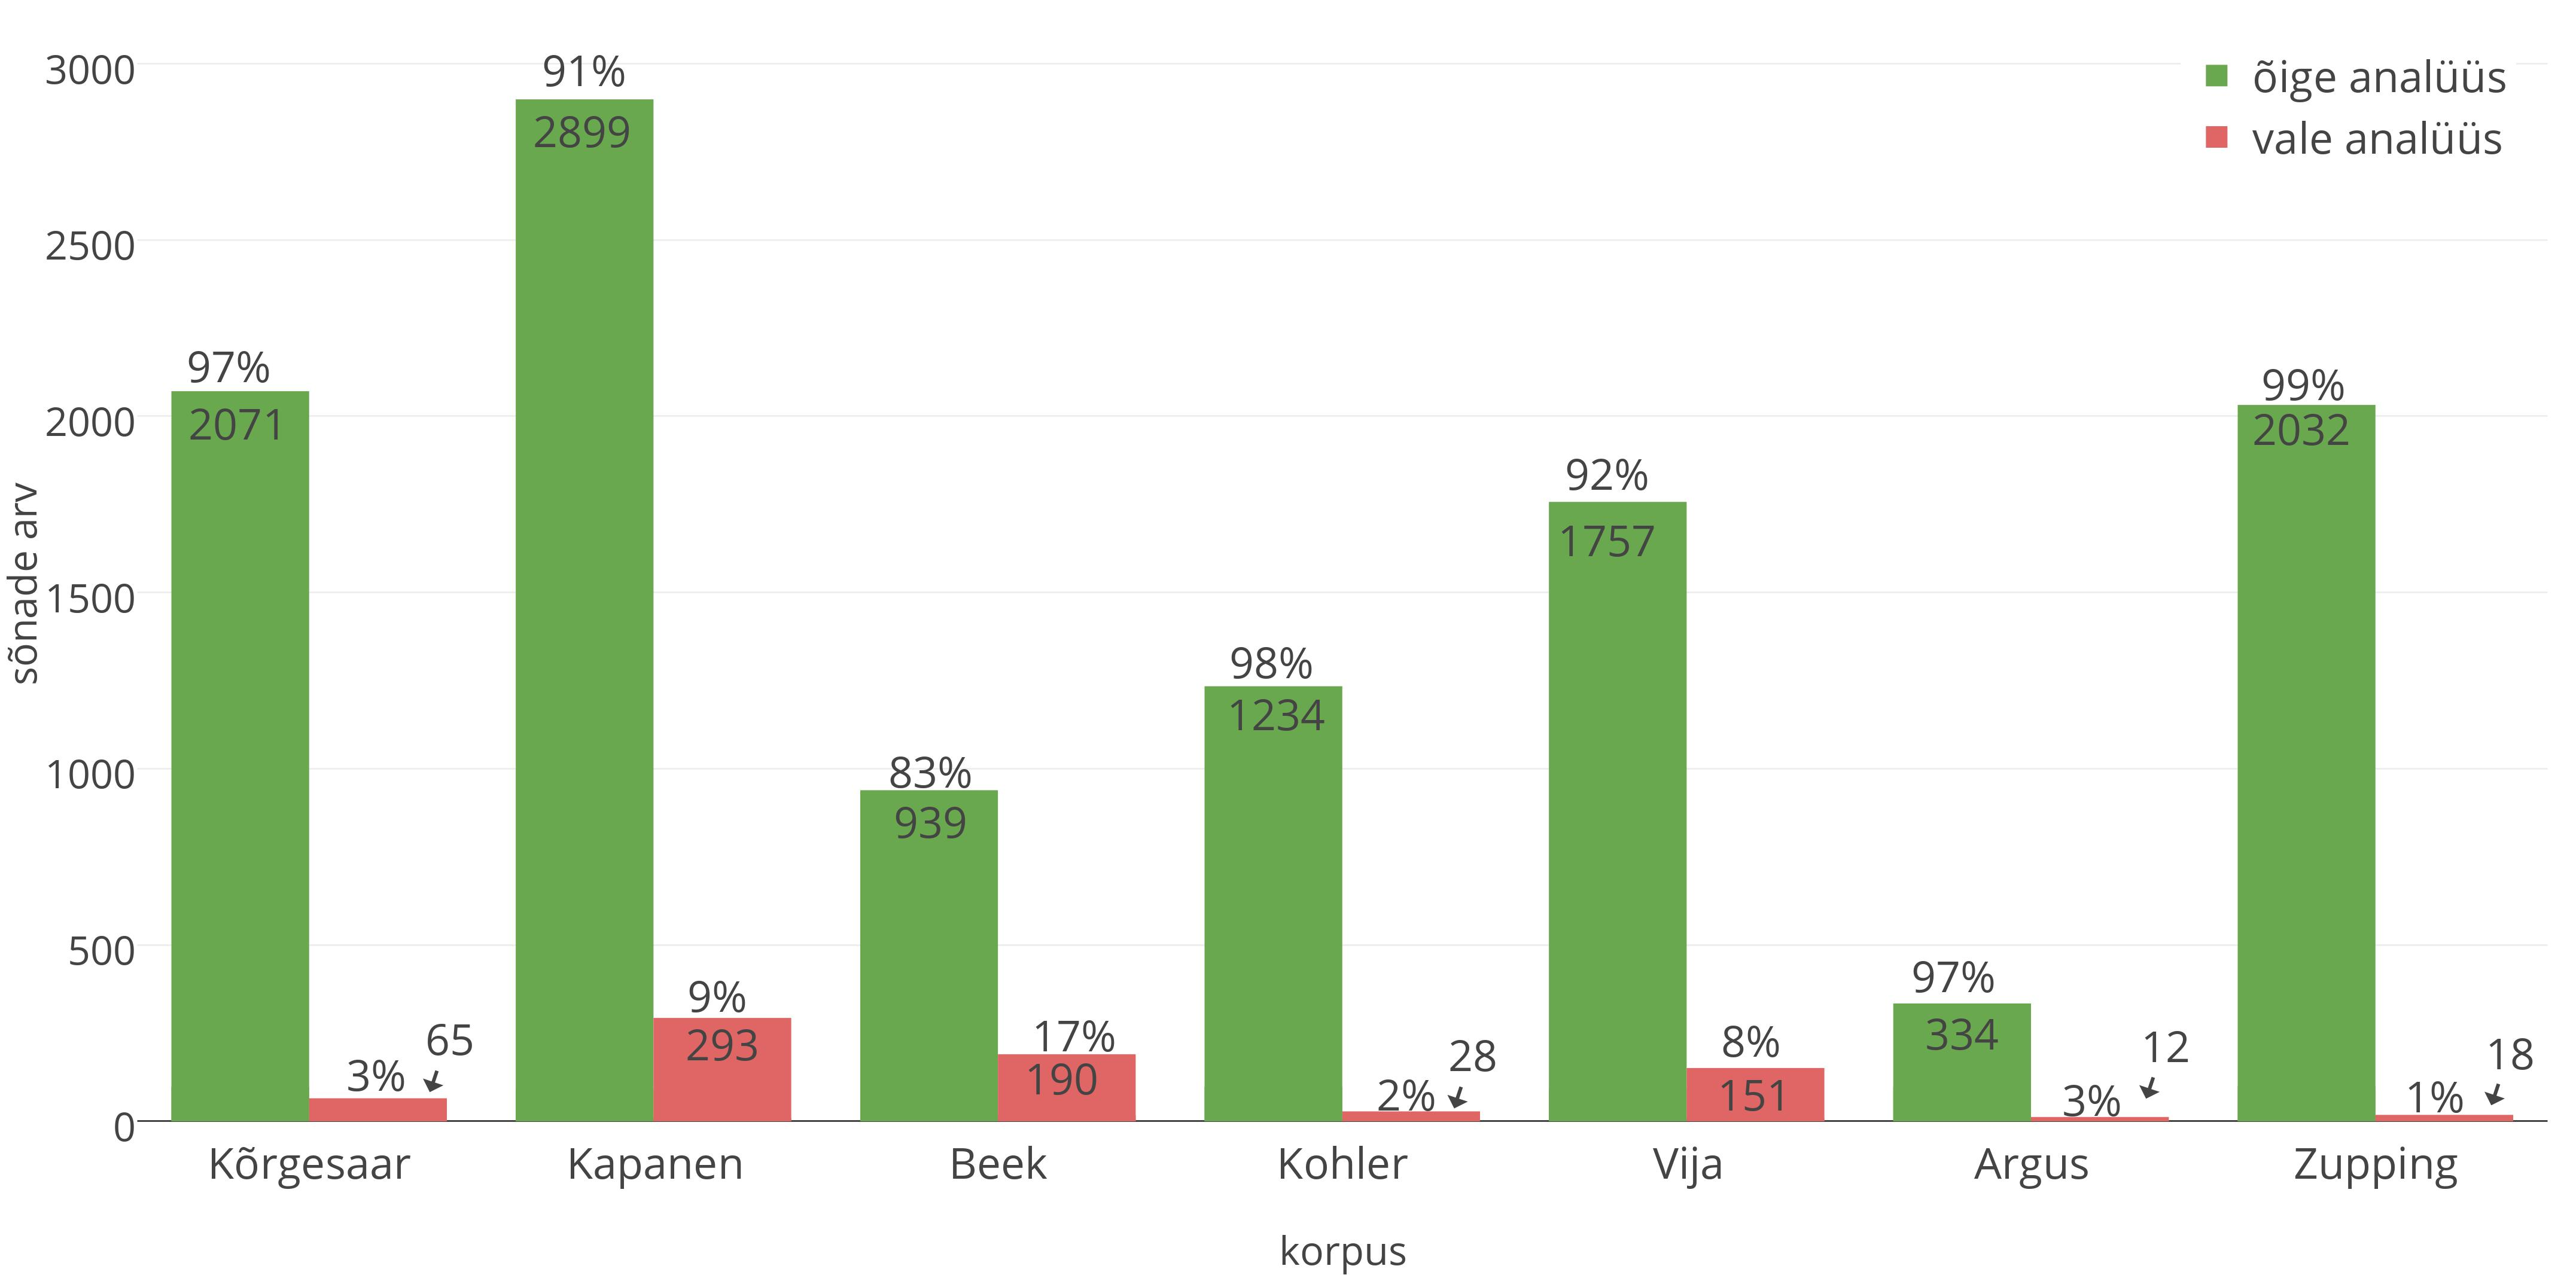
\includegraphics[width=\textwidth]{kasitsi_valed_oiged_crop}
    \caption{õige ja vale analüüsi saanud sõnad korpuse kaupa}
\end{figure}

Kõige paremad tulemused olid Zuppingu korpuses, kus keelematerjal pärineb lindistusest lapsega vanuses 4;2. Vale analüüsi saanud sõnu oli vaid 1\% ja õige analüüsi 99\% kõikidest analüüsi saanud sõnadest. Kohleri korpuses olid vale analüüsi saanud 2\% sõnadest (lapse vanus 1;11). Nii Arguse kui ka Kõrgesaare korpuses olid analüüsitud sõnadest 3\% saanud vale analüüsi (Argusel laps vanuses 1;8 ja Kõrgesaarel 1;3). Vija korpuse puhul (laps vanuses 1;7) oli vale analüüsi saanud 8\% kõikidest analüüsitutest sõnadest. Kapaneni korpuses (laps vanuses 1;3) oli 9\% analüüsi saanud sõnadest saanud vale analüüsi. Protsentuaalselt oli kõige enam vale analüüsi saanud sõnu (17\%) Beeki korpuses (laps vanuses 0;9). Siinkohal tuleks muidugi tähelepanu pöörata ka sellele, et selline järjestus võib tuleneda ka tahtmatust vanuselisest järjestusest -- kõige vähem vale analüüsi saanud sõnu on Zuppingi korpuses, kus lapse vanus on 4;2, ja kõige enam Beeki korpuses, kus lapse vanus on 0;9. Tegin kõikidest vale analüüsi saanud sõnadest sagedusloendi ja jagasin sõnad 5 erinevasse rühma.

\textbf{Esimese rühma} moodustavad onomatopeetilised sõnad: \emph{viu}, \emph{viuviu}, \emph{nämm}, \emph{amps}, \emph{mämmmämm}, \emph{mämm}, \emph{tapa}, \emph{summ}, \emph{pimm}, \emph{klõps}, \emph{pomm}, \emph{kiiga}, \emph{plaksu-plaksu}, \emph{patsu}, \emph{piiks-piiks-piiks-piiks}, \emph{piiks-piiks}, \emph{pats-pats-pats-pats}, \emph{amps}, \emph{kaak}, \emph{keps}, \emph{sulla}, \emph{kop}, \emph{mõmm}, \emph{põmm}, \emph{kaaga}, \emph{kõps}, \emph{patsu-patsu}, \emph{nämm}, \emph{pisspiss}, \emph{köhi}, \emph{aia}. 


\textbf{Teise rühma} moodustavad häälitsused ja sõnad, mille tähendusest pole võimalik aru saada ka konteksti olemasolul: \emph{paa}, \emph{eo}, \emph{änn}, \emph{tiks}, \emph{t}, \emph{pupe}, \emph{pigi}, \emph{op}, \emph{muks}, \emph{kookai}, \emph{kaka}, \emph{jää}, \emph{manni}, \emph{öö}, \emph{ämm}, \emph{mm}, \emph{a}, \emph{ä}, \emph{s}, \emph{emm}, \emph{mm}. \textbf{Kolmanda rühma} moodustavad pärisnimed, mis puuduvad morfoloogilise analüsaatori leksikonist: \emph{Tiibu}, \emph{Triibu}, \emph{Liisu}, \emph{Tups}, \emph{Tuksi}, \emph{Carlos}, \emph{Sirts}, \emph{Sirtsu}, \emph{Annika}, \emph{Antsu}, \emph{Pitsu}, \emph{Alari}.

\textbf{Neljanda rühma} moodustavad sõnad, mis saavad, kas vale lemma või sõnaliigi: 
\emph{mõmmi}, \emph{siuke}, \emph{venna}, \emph{tudu}, \emph{pai}, \emph{siukse}, \emph{nuku}, \emph{kalli-kalli}, \emph{kalli}, \emph{vot-vot}, \emph{tantsi-tantsi}, \emph{näri-näri}, \emph{mida-mida}, \emph{musi-musi}, \emph{kapp-kapp}, \emph{kapp-kapp-kapp-kapp}, \emph{istu-istu}, \emph{aitab-aitab}, \emph{aluspüksid-aluspüksid-aluspüksid}, \emph{ruttu-ruttu-ruttu}, \emph{väga-väga}, \emph{ja-ja-ja}, \emph{et-et-et}, \emph{tule-tule}, \emph{pisspissi}, \emph{mine-mine}. Siia alla kuuluvad ka sõnad nagu \emph{kuule}, \emph{palun}, \emph{näe}. Need sõnad on siin seetõttu, et need paiknevad verbi ja interjektsiooni piirimail ning oleksid justkui tekkinud täistähenduslike sõnade muutumise teel. 

\textbf{Viienda rühma} moodustavad sõnad, mis oma vormilt vigased (st on läbinud teatud täheteisendused) ja mida CHAT-failides kodeeritakse [\emph{= explanation}] abil: \emph{ütted} (\emph{ütled}), \emph{ükskold} (\emph{ükskord}), \emph{pilukat} (\emph{pirukas}), \emph{ea} (\emph{hea}), \emph{kah} (\emph{diktofon}), \emph{tee} (\emph{terve}), \emph{kesse} (\emph{kes see}), \emph{emmmee} (\emph{emme}), \emph{auh} (\emph{arvuti}), \emph{te} (\emph{see}), \emph{papa} (\emph{kõndima}), \emph{lau} (\emph{laud}), \emph{kiku} (\emph{diktofon}), \emph{kolla} (\emph{kollane}), \emph{teda} (\emph{seda}), \emph{täh} (\emph{aitäh}), \emph{laua} (\emph{laulma}), \emph{kuku} (\emph{luku}), \emph{kiigu} (\emph{kiik}), \emph{au} (\emph{arvuti}), \emph{olla} (\emph{alla}), \emph{määgu} (\emph{mänguasjad}), \emph{kukk} (\emph{trukk} või \emph{raamat}), \emph{koss} (\emph{koos}), \emph{kõrre} (\emph{kõrgel}), \emph{katte} (\emph{kätte}), \emph{kurki} (\emph{kurku}), \emph{noosi} (\emph{joonista}), \emph{kispi} (\emph{küpsis}), \emph{takku} (\emph{traktor}), \emph{ots} (\emph{otsas}), \emph{mammu} (\emph{mari}), \emph{äi} (\emph{ai}), \emph{utu} (\emph{lutt}), \emph{kiika} (\emph{kiikuda}), \emph{kass} (\emph{kastis}), \emph{kapi} (\emph{käbi}), \emph{takka} (\emph{traktor}), \emph{ussi} (\emph{sussid}), \emph{eita} (\emph{ei taha}), \emph{ängi} (\emph{mängib}), \emph{väigi} (\emph{värvi}), \emph{uu} (\emph{õun}), \emph{uksi} (\emph{nutikas}), \emph{toodi} (\emph{joonista}), \emph{tisse} (\emph{televiisori}), \emph{tahta} (\emph{tahan}), \emph{sea} (\emph{see}), \emph{raama} (\emph{raamat}), \emph{puusi} (\emph{pluusi}), \emph{puuniks} (\emph{pruuniks}), \emph{pusti} (\emph{püsti}), \emph{punnu} (\emph{punnis}), \emph{präägust}, \emph{pettu} (\emph{peitu}), \emph{palu} (\emph{palun}), \emph{memme} (\emph{me me}), \emph{märgi} (\emph{värvi}), \emph{mängu} (\emph{mänguasjad}), \emph{mähku} (\emph{mähe}), \emph{laadi} (\emph{lahti}), \emph{kuudi} (\emph{uurima}), \emph{kumme} (\emph{kolm}), \emph{ku} (\emph{diktofon}), \emph{koo} (\emph{koos}), \emph{kõne} (\emph{põnev}), \emph{kombe} (\emph{kombekas}), \emph{kiidu} (\emph{kiisu}), \emph{kii} (\emph{diktofon}), \emph{kat} (\emph{kaks}), \emph{kalju} (\emph{karu}), \emph{kaapi} (\emph{kapi}), \emph{boodi} (\emph{voodi}), \emph{aula} (\emph{laulda}), \emph{auk} (\emph{arvuti}), \emph{aru} (\emph{arvuti}), \emph{ala} (\emph{sajajalgne}), \emph{kipsist} (\emph{küpsist}), \emph{kiisupilt} (\emph{kiisu pilt}), \emph{keti} (\emph{kõdi}), \emph{lutu} (\emph{lutt}), \emph{kumme} (\emph{kummikud}), \emph{sala} (\emph{sajajalgne}), \emph{pillu} (\emph{piilub}), \emph{patt} (\emph{part}), \emph{panni} (\emph{banaanid}), \emph{paa} (\emph{maal}), \emph{olu} (\emph{orav}), \emph{oa} (\emph{orav}), \emph{süü} (\emph{süüa}), \emph{sunni} (\emph{sünnipäev}), \emph{punni} (\emph{punnis}), \emph{käia} (\emph{käima}), \emph{võta} (\emph{võtta}), \emph{õue} (\emph{õues}), \emph{maitse} (\emph{maitsevad}), \emph{koti} (\emph{kott}), \emph{mai} (\emph{mari}), \emph{aua} (\emph{koer}), \emph{voot} (\emph{vot}), \emph{Kate} (\emph{Kattre}).

Täielikult vigadeta morfoloogiliselt märgendatud korpus eeldab, et iga sõnavorm saab õige sõnaliigilise kuuluvuse, käändsõnade puhul õige arvu ja käände, verbide puhul õige arvu, isiku, tegumoe, aja, kõneviisi ja kõnelaadi. Õige analüüsi valimine läheb keeruliseks siis, kui sõna paikneb kahe sõnaliigi vahel või kasutatakse teise sõnaliigi funktsioonis. Suur osa kategooriatest on vormi põhjal üheselt määratavad, kuid on selliseid mitteühesuse tüüpe, mis valmistavad isegi käsitsi määramisel raskusi, nt käändsõnad ja verbid, mille vormidest arenevad adpositsioonid ja adverbid (nt \emph{kätte}, \emph{käes}, \emph{alates}), verbi ja adjektiivi piirimail paiknevad partitsiibid (nt \emph{surnud}, \emph{kadunud}) ning adverbi ja konjunktsioonide piirimail paiknevad sõnad (nt \emph{aga}, \emph{nagu}, \emph{kui}). Morfoloogilise analüüsi mõttes oleks hea, kui sellist piirimail asetsemist oleks võimalikult vähe ja seetõttu peaksid sõnaliigid olema kirjeldatud nii, et ka süntaksit saaks võimalikult otstarbekalt kirjeldada. (\citealp[102--104]{Sonaliik}; \citealp[627--631]{Sonaliik2}).

Uue meedia korpuses võeti morfoloogilisel märgendamisel kasutusele partikli sõnaliik. Partikkel on muutumatu mittetäistähenduslik sõna, millel on eelkõige suhtluslik ja emotsionaalne funktsioon. \citep[4]{UUSMEEDIA} Ka lapsekeele korpuse puhul tuleks mõelda mõne uue sõnaliigi kasutusele võtmise peale. Näiteks, mida teha esimesse rühma kuuluvate ehk onomatopeetiliste sõnadega? Onomatopoeetilistest sõnadest ei saa üle vaadata, sest need kuuluvad lapse esimeste sõnade hulka ja on hoidjakeeles väga sagedased. Reili Argus eristab helijäljenduslike sõnade hulgas ka \emph{imitatiive}, mis on onomatopoeetilised sõnad, mille häälikuline kuju võib olla varieeruv, kuid ei muutu morfoloogiliselt; või spontaanselt moodustatud leksikaalsed üksused, mille keskne omadus on helijäljendamine. Tüüpiliseks imitatiiviks on nt kiirabiauto signaali imiteeriv \emph{viuviu}, kõndmise väljendamiseks kasutatav \emph{tipa-tapa}. \citep[19--22]{IMITATIIV}

Lisaks sellele, et onomatopoeetiliste sõnade ja imitatiivide piir on hägune, on onomatopoeetilised sõnad ja imitatiivid ka lapse varases keelekasutuses sõnaliigililt mitmesed. \citep[20--21]{IMITATIIV} Eesti keele käsiraamat (VIIDE) jagab tähenduse järgi onomatopoeetilised sõnad interjektsioonide alla. Hennoste nimetab jällegi interjektsiooni sõnaliigiliseks prügikastiks, sest sinna on pandud kokku erinevad üksused. Hennoste arvates on onomatopoeetilised sõnad interjektioonide alla paigutatud sellepärast, et neil kaldeline foneetiline ja fonoloogiline struktuur ning nad paiknevad sõna ja mittesõna piirimail. \citep[67]{Hennoste} Näites 1 ja 2 jääb segaseks, kas laps kasutab imitatiive nimisõna või verbina:

(1)
\begin{description}
    \item *CHI: \textbf{addrr}, \textbf{drrr}, \textbf{brrr}
    \item *MOT: just, niimoodi sa õues sõidad vankriga \citep[27]{IMITATIIV}
\end{description}

(2)

\%comment: osutab autole paberil
\begin{description}
    \item *MOT: nii, tuled teen
    \item *MOT: sina tee katusele
    \item *CHI: \textbf{iiuiiu}
\end{description}
\%comment: Hendrik joonistab vilkureid \citep[28]{IMITATIIV}

Väidetakse, et enne presüntaktilist perioodi ongi raske sõnu liigitada ja sõnaliikidest saab alles siis rääkida, kui laps hakkab kasutama mitmesõnalisi väljendeid. Liigitusprobleemid tekivad eelkõige siis, kui sõnal puuduvad morfoloogilised ja süntaktilised tunnused. Kui lapse lausung pole pikem kui üks sõna, siis pole ka laiemast kontekstist kasu. \citep[27--29]{IMITATIIV} Vale analüüsi saanud sõnu hinnates jõudsin tõdemusele, et onomatopoeetilistele sõnadele on väga raske sõnaliigilist kuuluvust määrata, mitõttu paigutasin ``kirvemeetodil'' kõik helijäljenduslikud sõnad ühe rühma.



\newpage
\section{Edasine töö}
\newpage

\addcontentsline{toc}{section}{Kokkuvõte}
\section*{Kokkuvõte}

Seminaritöös kirjeldati korpuse olemust ja selle tähtsust keeleuurijale. Korpuse mõte on seisneb selles, et sealt võimalikult lihtsalt olulist infot kätte saada, aga kahjuks korpuste standardiseerimine ja loomine pole nii lihtne töö. Kõik algab algmaterjalist. 

Selle töö eesmärk oli lühidalt tutvustada ja näidata, et selleks, et lapsekeele korpust luua, tuleks transkriptsioonides esmalt selgeks teha, et mida ja kuidas märgendada. Kui see on selgeks tehtud, siis tuleks dialoogide transkribeerimisel sellest ka kinni pidada ja teha seda järjepidevalt. Eelmises peatükis kirjeldasin vaid mõningaid transkriptsioonidega seotud probleeme. Paraku on nii, et see esimene tase (transkriptsioon) mõjutab oluliselt vahepealseid tasandeid (standardiseerimine ja morfoloogilise info lisamine), mis omakorda mõjutavad lõpliku morfoloogiliselt märgendatud korpuse kvaliteeti.

\newpage
\cleardoublepage
\phantomsection
\addcontentsline{toc}{section}{Kasutatud kirjandus}
\bibliographystyle{dcu}
\bibliography{viited}

\end{document}


